\documentclass{ctexart}
\usepackage[utf8]{inputenc}

\title{固体物理课堂笔记}
\author{Yinjia Chen }
\date{\today}

\usepackage{natbib}
\usepackage{graphicx}
\usepackage{float}
\usepackage{amsfonts}
\usepackage{amsmath}
\usepackage{amssymb}
\usepackage{subcaption}
\begin{document}

\maketitle
\tableofcontents
\newpage
\section{简介}
本文是固体物理的自学笔记。

本课程主要的研究对象是所谓的理想晶体,理想晶体具有几个特征:
\begin{enumerate}
    \item 晶体向各个方向无限延申(这个近似实际上很有道理,因为一般的原胞尺度约为$10^{-10}m$,而一般的晶体大小在$10^{-3}m$量级左右);
    \item 晶体无缺陷
\end{enumerate}

我们研究晶体至始至终贯穿晶体的周期性,从原子(离子)实静止到原子(离子)实的振动再到电子运动,对理想晶体的基本性质做了介绍,具体如下:
\begin{itemize}
    \item 原子静止$\xrightarrow{\quad\quad\quad\quad\ }$ 晶体结构
    \item 晶格振动 $\xrightarrow{B-K\text{边界条件}}$ 声子的色散关系$\omega(q)$
    \item 电子运动 $\xrightarrow{Bloch\text{周期势场}}$ 电子的色散关系$E(k)$\footnote{我们从金属到能带理论再到半导体的顺序展开}
\end{itemize}

同时,晶体的求解是一个典型的多体问题,多体问题的复杂性告诉我们需要先对物理现象进行抽象,抽出决定因素后进行物理建模,具体如下:
\begin{itemize}
    \item 从原子角度上来说,我们主要采用晶格动力学理论并提出声子的概念。基于此,我们使用了简谐近似(将原子的振动近似看作简谐振子)和最近邻近似(只考虑最相邻原子的相互作用)
    \item 从电子角度上来说,最早科学家提出自由电子理论来解释固体中的一些结论,但是自由电子理论忽略了原子核对电子的势能。因此作为修正,我们将原子核的周期势场看作自由电子理论的微扰,由此我们可以得到能带理论。
\end{itemize}


\section{晶体结构}
    \subsection{晶体结构,晶胞,晶系}
晶体分为单晶体、多晶体、液晶。单晶体指的是大尺度下同样有序;多晶体指的是小尺度(约10$\mu m$)有序;液晶指的是在一定的温度下,在一维或二维的条件下有序。本笔记主要考虑单晶体。

晶体具有许多宏观特性:自范性、解理性、晶面角守恒定律、各向异性、均匀性、对称性,同时有固定的熔点以及最低内能。这些宏观特性都是源于晶体内部结构的周期性。

下面对本门课程的若干概念予以说明:
\begin{itemize}
    \item 理想晶体是由重复单元周期性排列而成。我们称最小的重复单元为基元(basis),此时我们可以将基元抽象为一个点,称为格点(lattice point);格点的有序周期性排列称为点阵/晶格。
    \item 基元分为两种。一种基元只含有一个粒子,称为布拉维格子(Blavais lattice);而一种基元含有大于一个粒子,称为复格子(compound lattice)。可以明显看出,复格子一定是多个布拉维格子的嵌套。
    
        \begin{figure}[H]
        \centering
        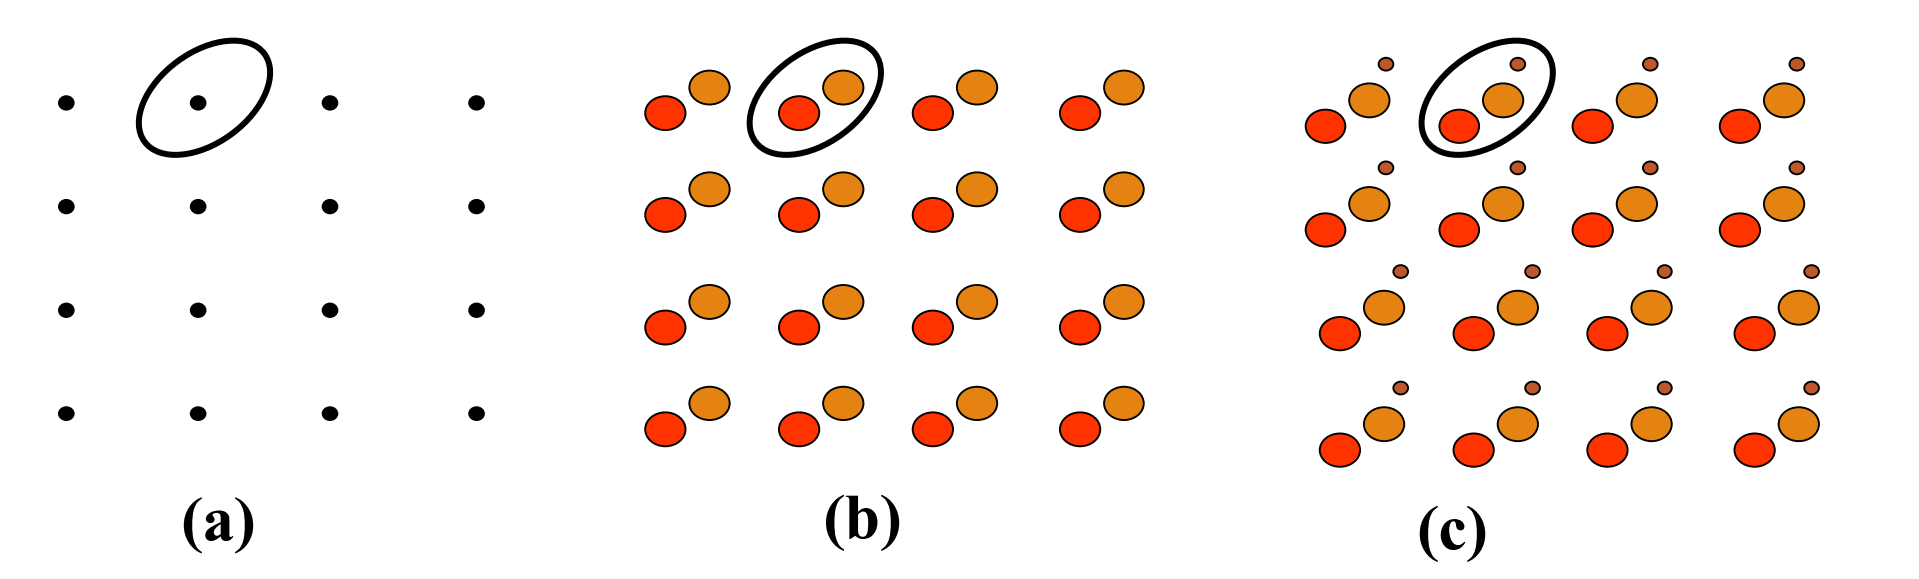
\includegraphics[width=0.9\textwidth]{figure/lattice.png}
        \caption{布拉维格子与复格子的例子}
        \label{fig:lattice}
    \end{figure}

    \item 布拉维格子还能从格矢的角度阐述。格矢就是以某个格点为原点,线性无关的基底构成的能够描述晶格平移的矢量。显然布拉维格子还能表述为格矢全部端点的集合。
    \item 以任意格点为原点向邻近的格点作三条不共面的矢量,矢量构成的平行六面体我们称之为原胞(Primitive Cell)。假设矢量分别为$\Vec{a_1},\Vec{a_2},\Vec{a_3}$,那么平行六面体的面积为$\Omega=a_1\cdot(a_2\times a_3)$。原胞的特点是只有顶点上有格点,内部、棱上都没有格点,此时整个原胞只含有一个格点。
    \item 由于原胞基矢的选择不唯一,因此原胞也不唯一,为了统一构造方法,我们可以采用Wigner-Seitz Cell 的构造方法,构造方法如图\ref{fig:W-S Cell}
    
        \begin{figure}[H]
        \centering
        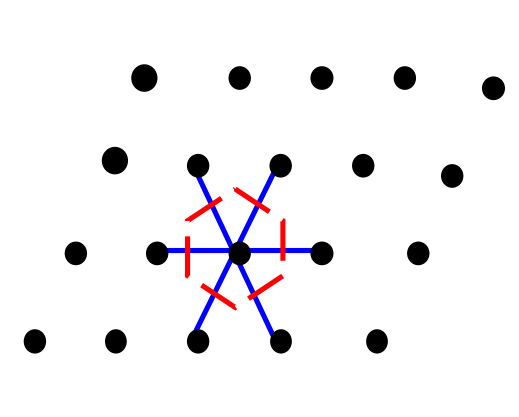
\includegraphics[width=0.5\textwidth]{figure/W-S Cell.png}
        \caption{W-S Cell构造实例}
        \label{fig:W-S Cell}
    \end{figure}
    
    \item 有时,构造出来的原胞对称性并不好,因此我们引入晶胞的概念。晶胞的基矢要求尽量沿着空间对称轴的方向,图\ref{fig:crystalCell}是一个简单的例子,可以看出晶胞不止包含一个格点。
    
        \begin{figure}[H]
        \centering
        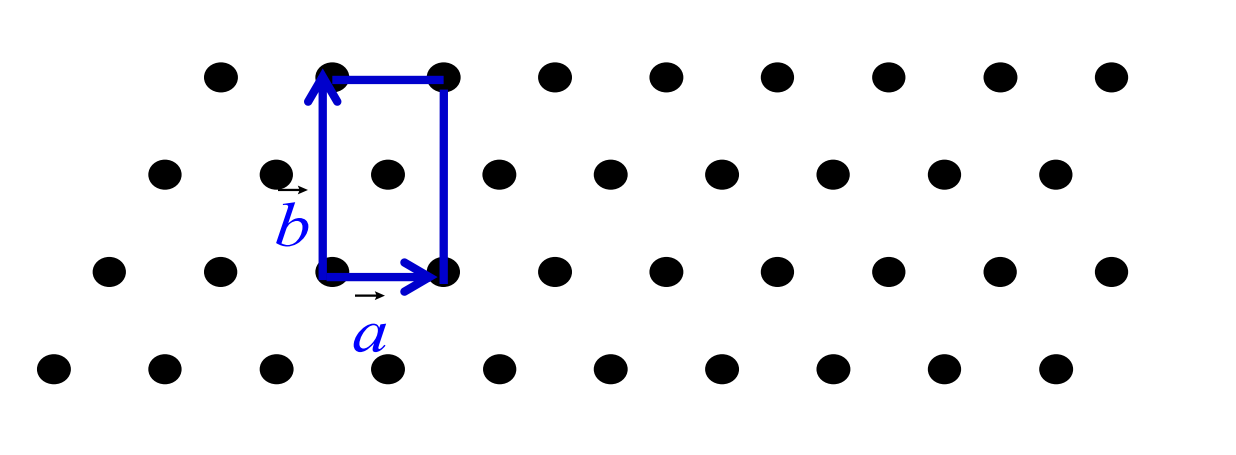
\includegraphics[width=0.9\textwidth]{figure/crystal cell.png}
        \caption{晶胞构造的简单例子}
        \label{fig:crystalCell}
    \end{figure}
    \end{itemize}
    

    关于确定原胞,有几个注意事项:
    \begin{itemize}
        \item 判断原子之间是否等价。所谓等价原子就是原子周围所处环境是完全相同的
        \item 不等价原子作为基元;不同基元中等价的原子作为格点;基矢只考虑等价的原子
    \end{itemize}
    
    可以看图\ref{fig:example}的例子。可以看到左图所有格点都是等价的;而右侧有两类不等价的原子,因此原胞基矢的选择也会不同。
     \begin{figure}[H]
    \centering
    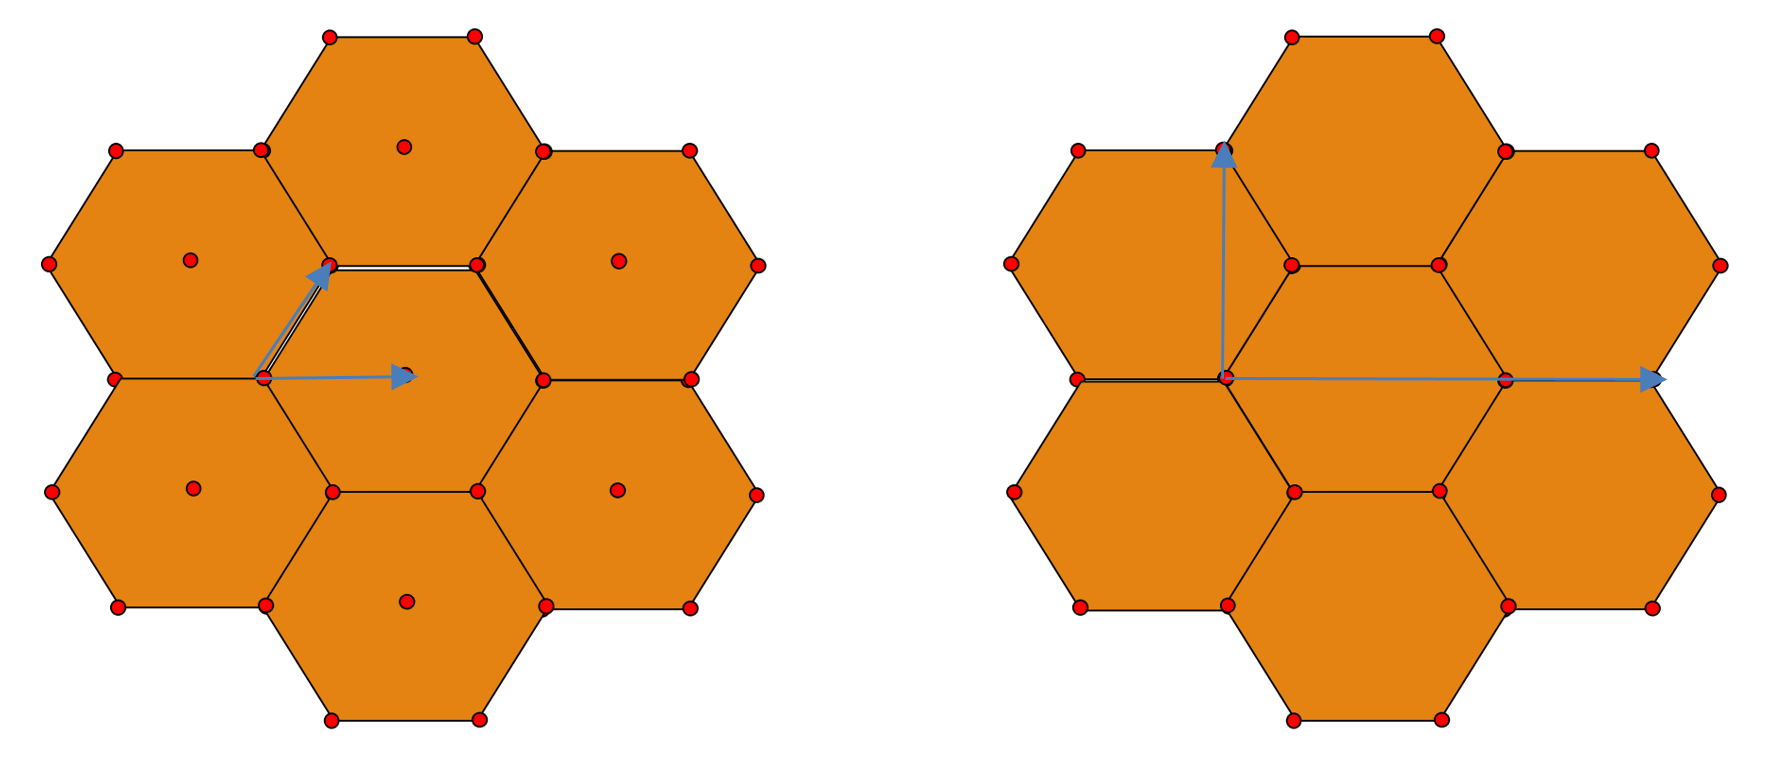
\includegraphics[width=0.9\textwidth]{figure/CH1_example.png}
    \caption{原胞与原胞基矢确定的例子}
    \label{fig:example}
    \end{figure}
    
    最后我们介绍和配位数的概念。在课程中,我们往往会求各种密堆积的体积利用率。配位数的定义是一个原子周围最近邻的原子数,它描述一种结构的密集程度。如图\ref{fig:coordinatenumber_example},从中我们可以看到,对于一维密堆积结构,其配位数为2;而对于二维密堆积结构,其配位数为6.
    \begin{figure}[H]
        \begin{subfigure}{0.5\textwidth}
        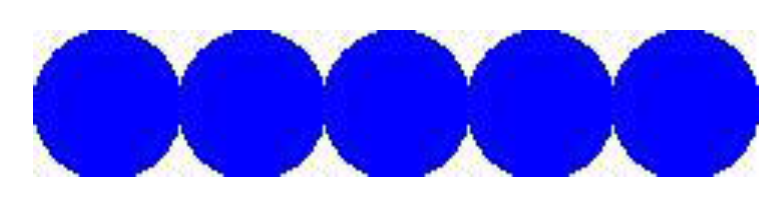
\includegraphics[width=0.9\linewidth, height=5cm]{figure/CN_1D.png} 
        \caption{一维密堆积}
        \label{fig:CN_1D}
        \end{subfigure}
        \begin{subfigure}{0.5\textwidth}
        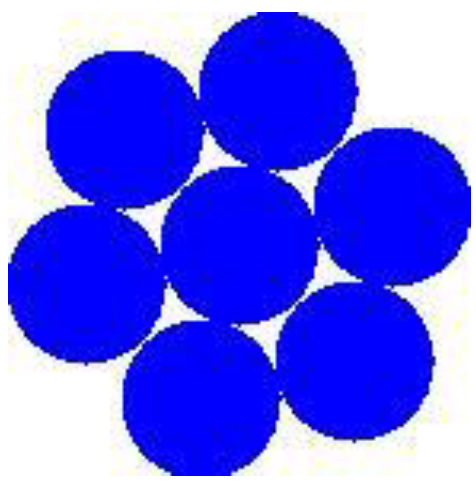
\includegraphics[width=0.9\linewidth, height=5cm]{figure/CN_2D.png}
        \caption{二维密堆积}
        \label{fig:CN_2D}
        \end{subfigure}
        
        \caption{配位数的两个简单例子}
        \label{fig:coordinatenumber_example}
        \end{figure}
    
    
    
    \subsection{典型的晶体结构}
    本节我们基于上节的概念,对一些典型的晶体结构进行介绍,本节的框架如图\ref{fig:classiccrystalstructure}:
    \begin{figure}[H]
        \centering
        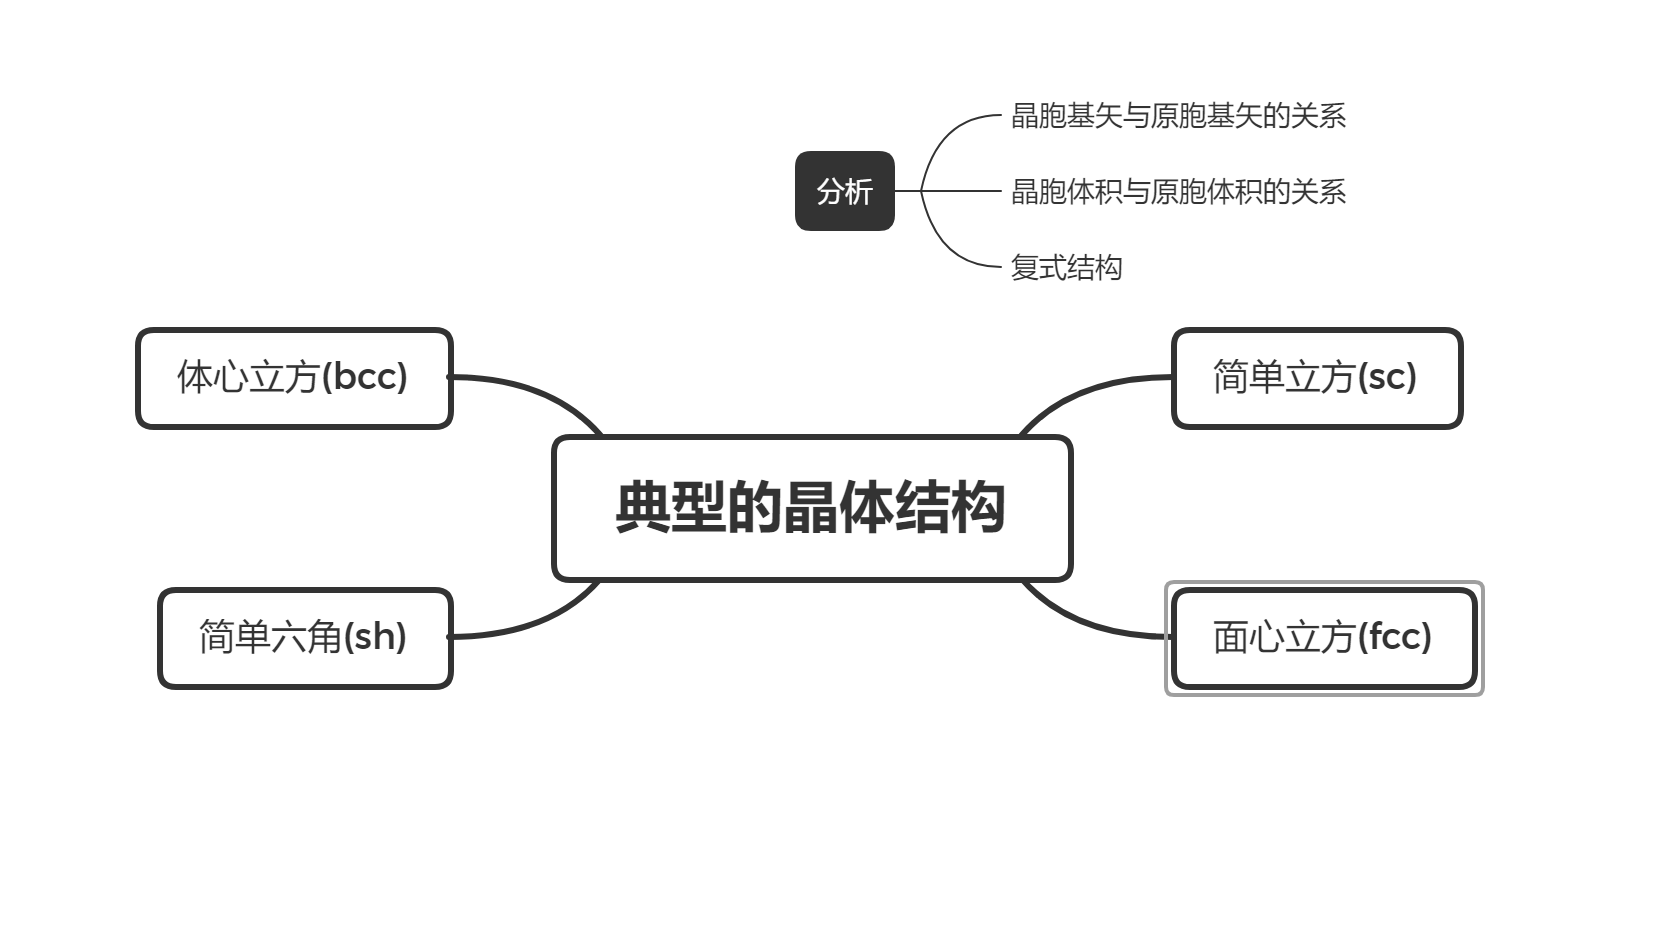
\includegraphics[width=0.9\textwidth]{figure/classiccrystalstructure.png}
        \caption{典型的晶体结构框架}
        \label{fig:classiccrystalstructure}
    \end{figure}
    
    首先我们考虑简单立方。由于简单立方的晶胞和原胞是重合的,自然其原胞基矢和晶胞基矢也是重合的,两者的体积也是相等的。简单立方的经典复式结构有两种:一种是CsCl结构,两个简单立方相互嵌套,其中$Cs^+$离子处于$Cl^-$离子的体心位置,由图可知,该结构两个离子的配位数都为8;
    \begin{figure}[H]
        \centering
        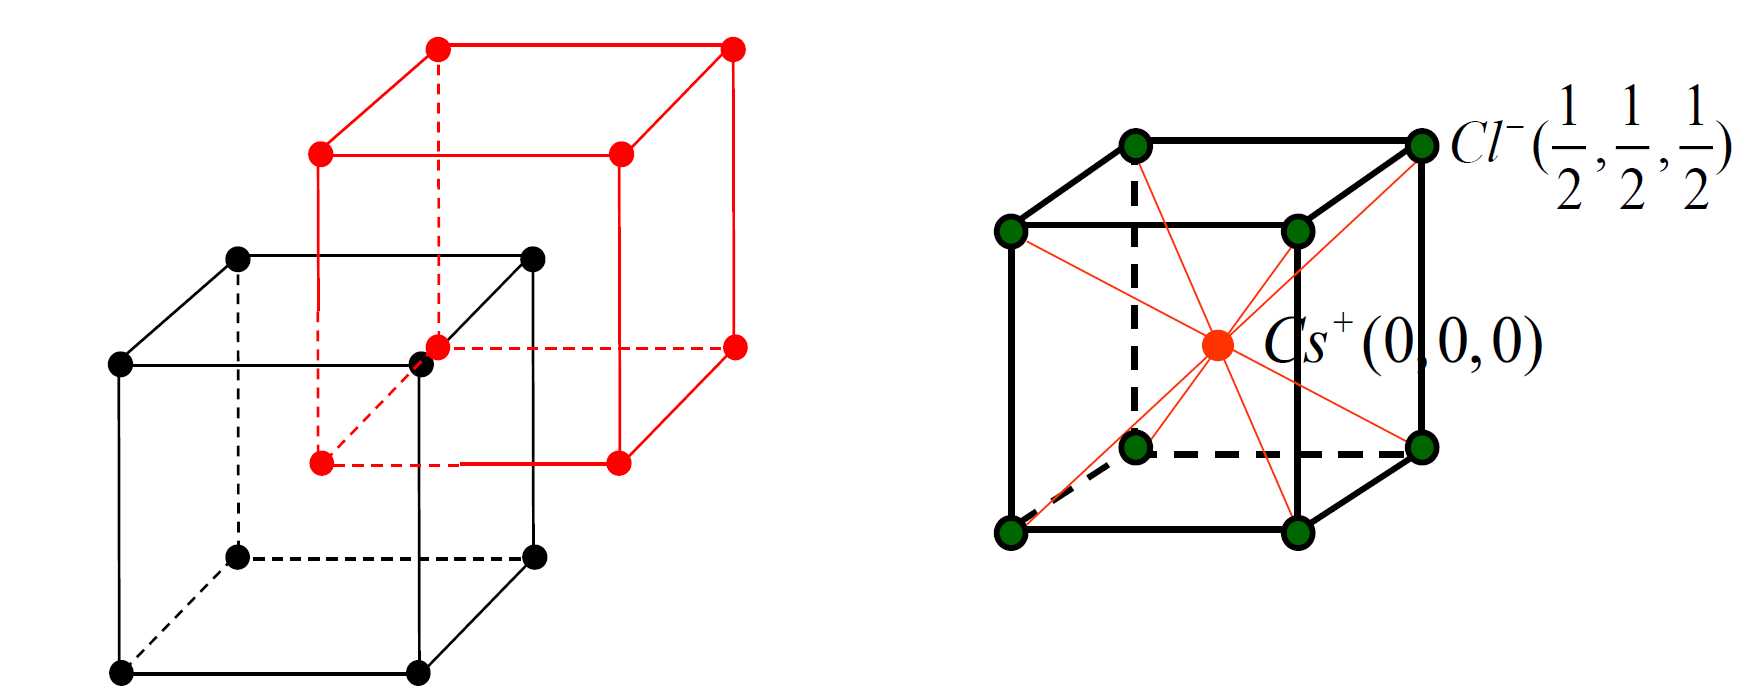
\includegraphics[width=0.9\textwidth]{figure/sc_CsCl.png}
        \caption{CsCl型结构的晶胞}
        \label{fig:CsCl}
    \end{figure}
    
    
    还有一种是钙钛矿$ABO_3$结构,如图\ref{fig:ABO3}这是5个简单立方互相嵌套,其中$B$离子处于$A$离子的简单立方的体心,三个$O^{-2}$离子的简单立方,分别位于于$A$离子简单立方的面形位置。考虑该结构的配位数,对于$A$离子来说,$O^{-2}$离子排布在面心的位置,因此应该是一个密堆积,配位数为12;对于$B$离子,我们可以发现$O^{-2}$离子围绕在它周围是一个八面体,因此配位数为6;对于$O^{-2}$离子来说,由于它位于面心,因此我们可以知道它的配位数为6。
    
    
        \begin{figure}[H]
        \begin{subfigure}{0.5\textwidth}
        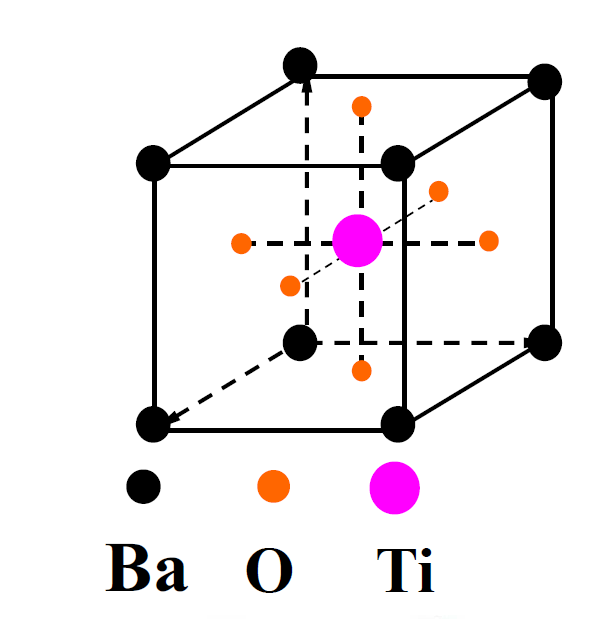
\includegraphics[width=0.9\linewidth, height=5cm]{figure/sc_ABO3_1.png} 
        \caption{$BaTiO_3$晶胞}
        \label{fig:sub_ABO3_1}
        \end{subfigure}
        \begin{subfigure}{0.5\textwidth}
        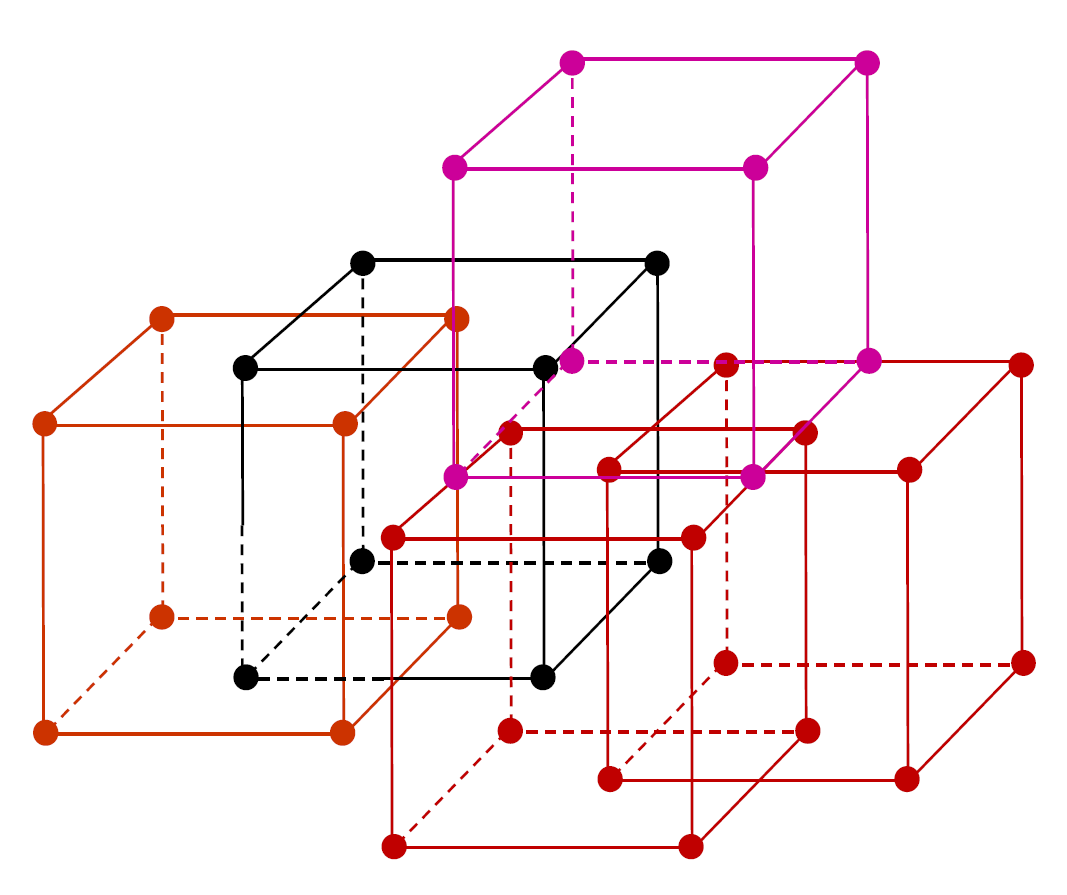
\includegraphics[width=0.9\linewidth, height=5cm]{figure/sc_ABO3_2.png}
        \caption{钙钛矿型复格子的嵌套过程}
        \label{fig:sub_ABO3_2}
        \end{subfigure}
        
        \caption{钙钛矿型($ABO_3$型)结构的晶胞}
        \label{fig:ABO3}
        \end{figure}
    
    随后我们考虑面心立方结构。令晶格常数为a,由于面心立方的晶胞含有4个粒子,因此其原胞基矢与晶胞基矢并不一样,根据图\ref{fig:fcc},我们知道原胞基矢$\Vec{i},\Vec{j},\Vec{k}$与晶胞基矢$\Vec{a_1},\Vec{a_2},\Vec{a_3}$的关系为:
    \begin{align}
        \begin{split}
            \Vec{a_1}=&\frac{a}{2}(\Vec{j}+\Vec{k})\\
            \Vec{a_2}=&\frac{a}{2}(\Vec{i}+\Vec{k})\\
            \Vec{a_3}=&\frac{a}{2}(\Vec{i}+\Vec{j})
        \end{split}
    \end{align}
    
    由上式,我们可以得到原胞的体积为:
    \begin{align}
        \begin{split}
            \Omega=&\Vec{a_1}\cdot(\Vec{a_2}\times\Vec{a_3})\\
            =& \frac{a^3}{8}\begin{vmatrix}
            0&1&1\\
            1&0&1\\
            1&1&0
            \end{vmatrix}\\
            =&\frac{a^3}{4}
        \end{split}
    \end{align}
    
    \begin{figure}[H]
        \centering
        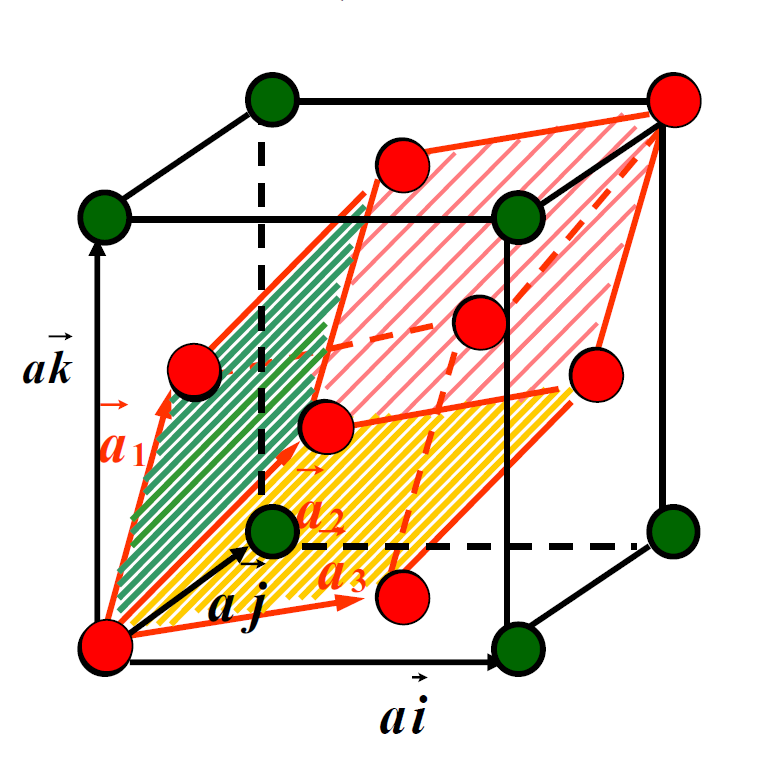
\includegraphics[width=0.6\textwidth]{figure/fcc.png}
        \caption{面心立方晶胞矢量与原胞基矢之间的关系}
        \label{fig:fcc}
    \end{figure}
    可以看到原胞的体积是晶胞体积的$\frac{1}{4}$。随后我们讨论面心立方的三种复式结构:NaCl型,金刚石型和闪锌矿型结构。如图\ref{fig:NaCl},我们可以知道氯化钠型结构是两个面心立方晶胞沿某个晶胞基矢方向的$\frac{1}{2}$嵌套而成。并且可以发现两种原子的配位数都为6。
    \begin{figure}[H]
        \centering
        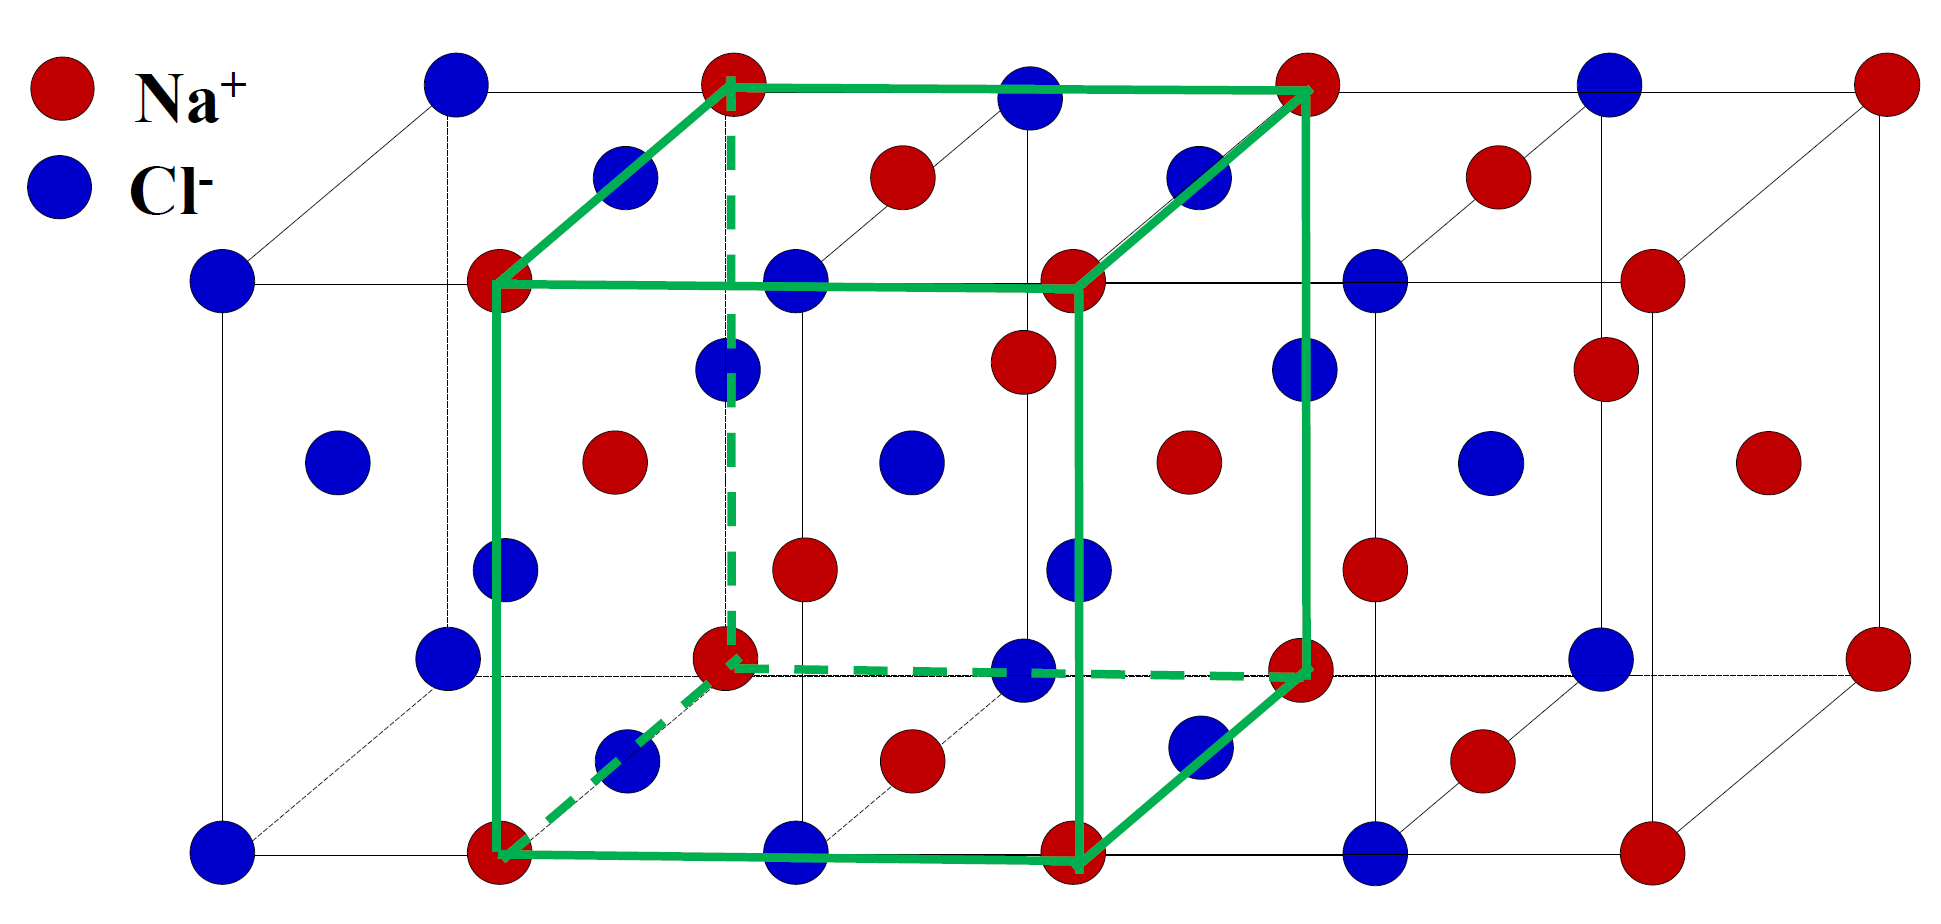
\includegraphics[width=0.9\textwidth]{figure/fcc_NaCl.png}
        \caption{NaCl结构的晶胞}
        \label{fig:NaCl}
    \end{figure}
    
    随后我们讨论金刚石型和闪锌矿型的结构。如图\ref{fig:diamond},我们可以知道,金刚石晶胞表面的原子核晶胞内的原子环境是不同的,因此金刚石结构是两个面心立方沿某条立方体体对角线的$\frac{1}{4}$嵌套而成。而闪锌矿型晶胞就是将金刚石两个同种原子的面心立方换成了不同原子而已,其结构没有变化。
     \begin{figure}[H]
        \begin{subfigure}{0.5\textwidth}
        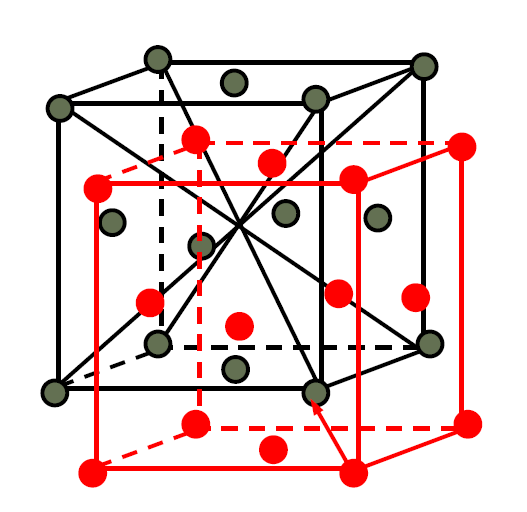
\includegraphics[width=0.9\linewidth, height=5cm]{figure/fcc_diamond_1.png} 
        \caption{金刚石型结构和闪锌矿型结构复格子的嵌套过程}
        \label{fig:sub_diamond_1}
        \end{subfigure}
        \begin{subfigure}{0.5\textwidth}
        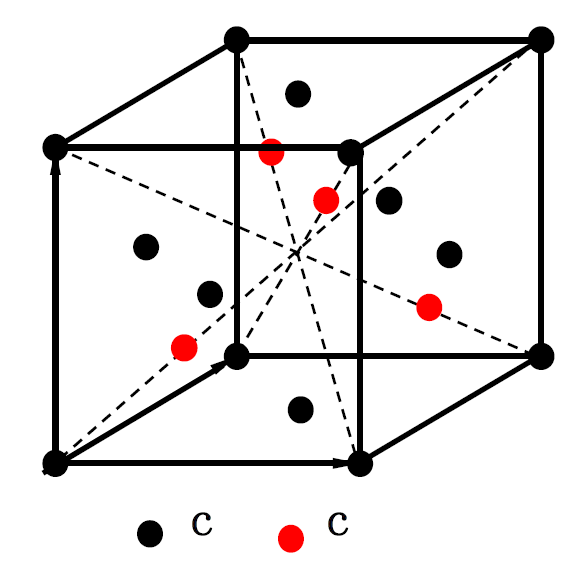
\includegraphics[width=0.9\linewidth, height=5cm]{figure/fcc_diamond_2.png}
        \caption{金刚石型结构晶胞}
        \label{fig:sub_diamond_2}
        \end{subfigure}
        
        \caption{金刚石型和闪锌矿型结构的晶胞}
        \label{fig:diamond}
        \end{figure}
    随后我们讨论体心立方,如图\ref{fig:bcc}。我们可以发现晶胞内包含两个等价原子,并且晶格矢量$\Vec{a_1},\Vec{a_2},\Vec{a_3}$,和原胞基矢$\Vec{i},\Vec{j},\Vec{k}$满足以下关系:
    \begin{align}
        \begin{split}
            \Vec{a_1}=&\frac{a}{2}(-\Vec{i}+\Vec{j}+\Vec{k})\\
            \Vec{a_2}=&\frac{a}{2}(\Vec{i}-\Vec{j}+\Vec{k})\\
            \Vec{a_3}=&\frac{a}{2}(\Vec{i}+\Vec{j}-\Vec{k})
        \end{split}
    \end{align}
    
    同理,原胞的体积为$\frac{1}{2}a^3$,是晶胞体积的一半。
    \begin{figure}[H]
        \centering
        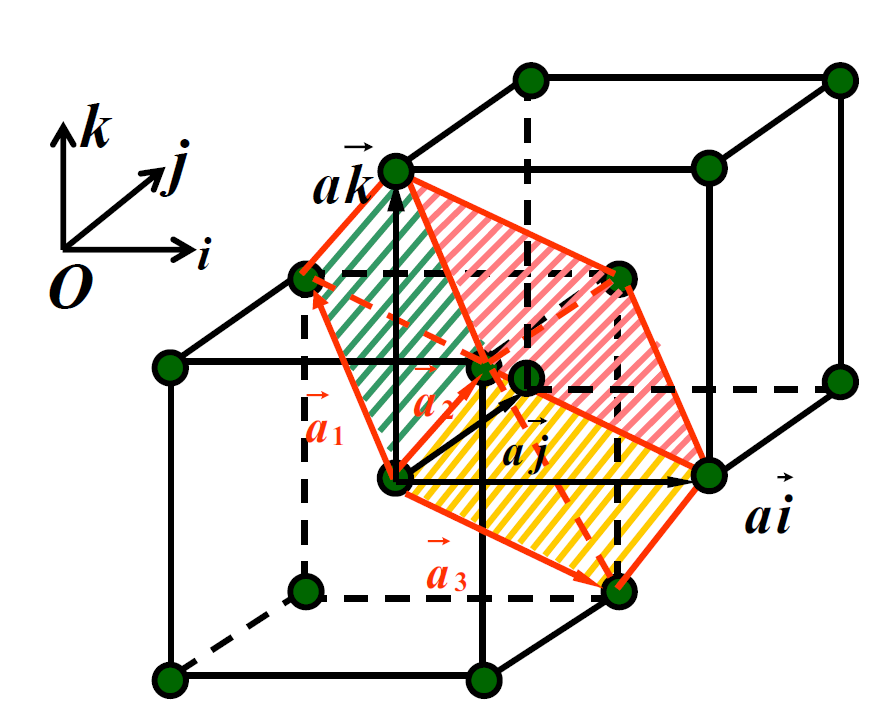
\includegraphics[height=\dimexpr\pagegoal-\pagetotal-4\baselineskip\relax,
  width=\textwidth,
  keepaspectratio]{figure/bcc.png}
        \caption{体心立方晶胞基矢与原胞基矢的关系}
        \label{fig:bcc}
    \end{figure}
    
    \subsection{晶列和密勒指数}
    由于晶体具有周期性结构,因此我们总可以将它们看成是一组平行直线或平行平面。由格点连线组成的直线称作晶列,由格点连线构成的平面称作晶面。首先考虑晶列,显然,晶列具有以下性质:
    \begin{itemize}
        \item 晶列上格点分布是周期性的;
        \item 平行晶列构成晶列族,晶列族包含所有的格点;
        \item 晶列族中的每一条晶列上,格点分布都是相同的;
        \item 在同一平面内,相邻晶列间的距离相等。
    \end{itemize}
    
    既然晶列可以构成周期性的晶体,那么在实际的工作中,标记晶列的方向或者是晶面的方位是十分必要的。并且,我们标记的往往是晶列族的方向而不是单一晶列的方向。
    
    取晶列上的一个格点为原点O,晶列上其它任意格点A的位矢为\footnote{其实这个定义不用那么复杂,取任意一个点作为原点O即可,只要晶列对应矢量能够被分解为晶胞基矢的线性组合就行了。}:
    \begin{equation}
        \Vec{OA}=m'\Vec{l_1}+n'\Vec{l_2}+p'\Vec{l_3}
    \end{equation}
    
    其中,$\Vec{l_1},\Vec{l_2},\Vec{l_3}$是晶胞基矢坐标系,随后为了表示的唯一性,我们将$m',n',p'$化为互质的整数$m,n,p$,记作$[m,n,p]$,比如立方晶胞的一个晶列位矢可以表示成:
    \begin{equation}
        \frac{1}{4}\Vec{a_1}+\frac{1}{4}\Vec{a_2}+\frac{1}{4}\Vec{a_3}
    \end{equation}
    
    根据定义,该晶列位矢对应的晶列指数为[1,1,1]。如果出现负指数,我们常常将负号置于指数的顶部,如$[\Bar{1},1,1]$等。

    而对于晶面,我们也有类似的指数,称作密勒指数。它是这样定义的:以晶胞基矢方向为坐标轴简历坐标系,晶面在3个方向的截距分别为$r\Vec{a},s\Vec{b},t\Vec{c}$,则将此3个系数的倒数:$\frac{1}{r},\frac{1}{s},\frac{1}{t}$约成互质整数$h,k,l$,并用圆括号表示,记作(h,k,l)
    
    但是对于六角晶胞,我们往往不使用三指数的密勒指数。因为在三指数的表示下,等效晶面的表示形式往往不相似,如图\ref{fig:hexagonalsystem1}。我们可以发现:根据对称性,AA'B'B和BCC'B'一定是等效晶面,但是AA'B'B的三指数密勒指数是$(1,\Bar{1},0)$;而BCC'B'的三指数密勒指数是(1,0,0),两者并没有相似性,这就给判断等效晶面带来不便性。
    \begin{figure}[H]
        \centering
        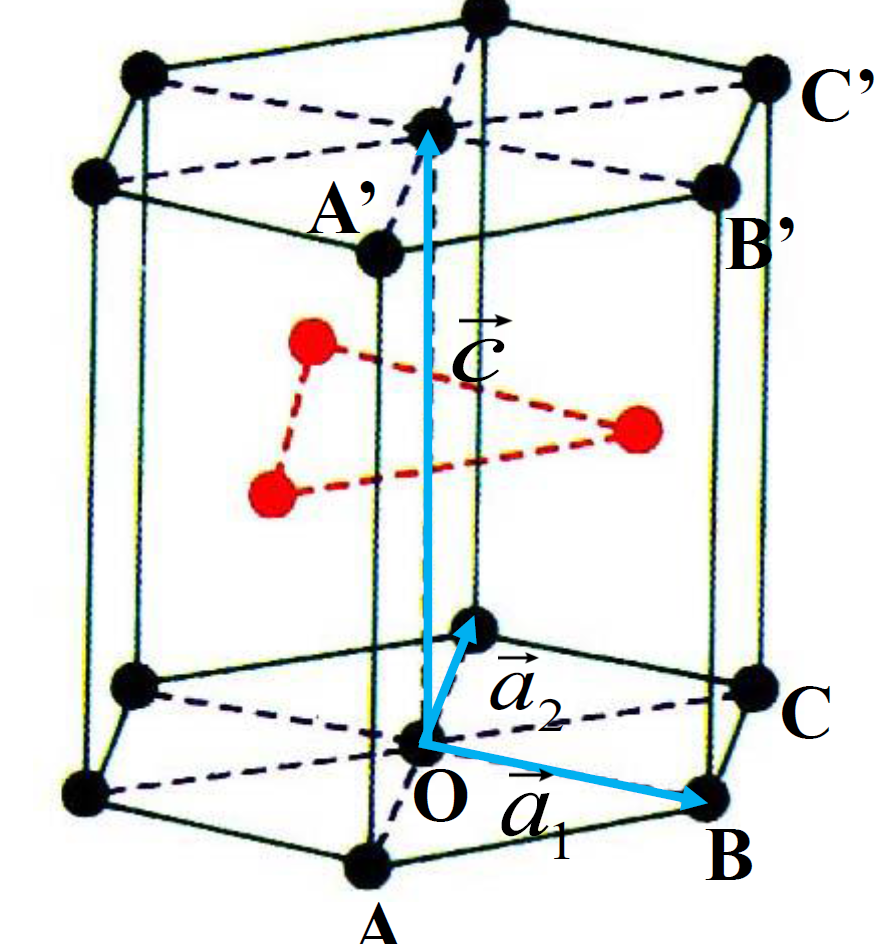
\includegraphics[width=0.5\textwidth]{figure/Hexagonal system.png}
        \caption{六角晶胞的三指数密勒指数晶胞基矢}
        \label{fig:hexagonalsystem1}
    \end{figure}
    
    因此我们引入四指数的密勒指数。如图\ref{fig:hexagonalsystem2},我们引入四个坐标矢量:$\Vec{a_1},\Vec{a_2},\Vec{a_3},\Vec{c}$,可以从图中看出,坐标矢量一定有关系:$\Vec{a_1}+\Vec{a_2}=-\Vec{a_3}$,因此四指数的坐标矢量是线性相关的,但是这样做的好处就是使得等效晶面的形式相似。比如等效晶面AA'B'B和BCC'B',前者的密勒指数为$(1,\Bar{1},0,0)$,后者的密勒指数为$(1,0,\Bar{1},0)$
    
        \begin{figure}[H]
        \centering
        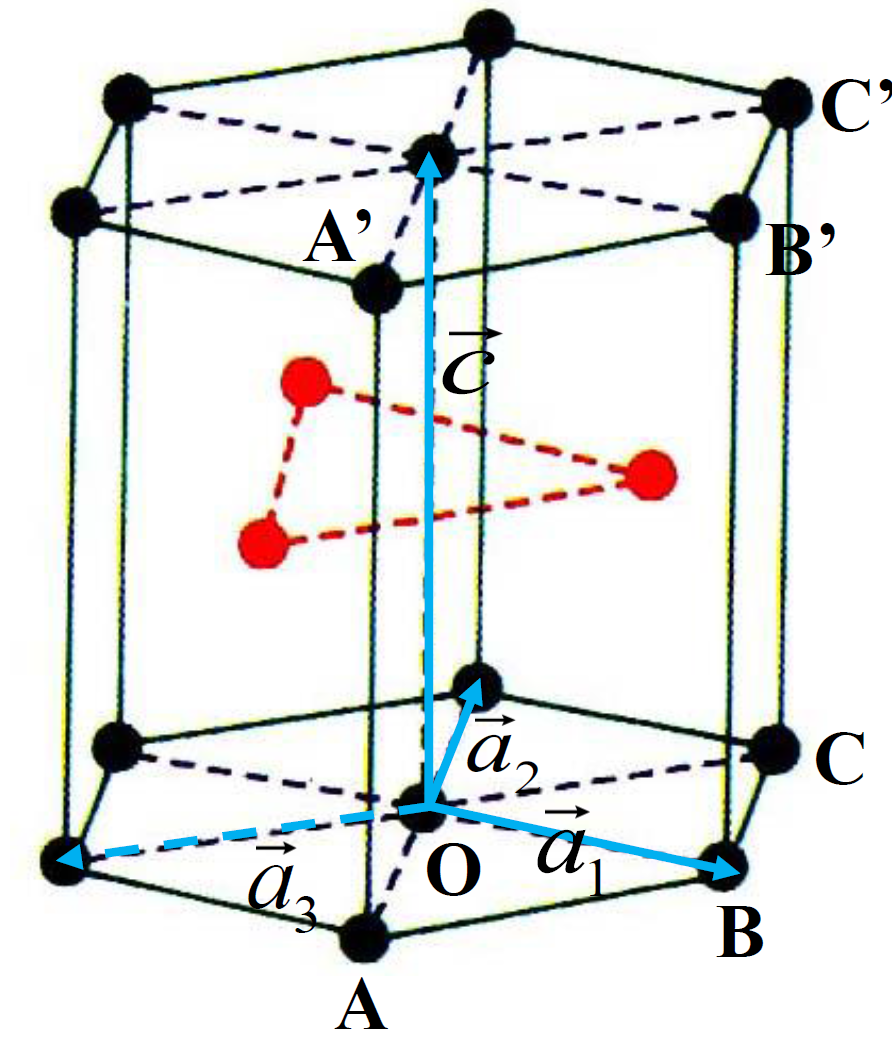
\includegraphics[width=0.5\textwidth]{figure/Hexagonal system2.png}
        \caption{六角晶胞的四指数密勒指数晶胞基矢}
        \label{fig:hexagonalsystem2}
    \end{figure}
    
    还有一些有关晶列和晶面的思考题:
    \begin{enumerate}
        \item 我们可以证明,对于立方晶系,$(h,k,l)$晶面与$[h,k,l]$晶列正交。证明的简单思路如下:根据定义,我们可以令晶列矢量为:
       \begin{equation}
            \Vec{OD}=h\Vec{a}+k\Vec{b}+l\Vec{c}
       \end{equation} 
       在高等数学中,我们知道直线与平面的正交等价为这条直线与平面上的任意两条不共线的直线正交。于是我们考察晶面上与晶胞表面相交的两个矢量。根据定义,这两个矢量可以表示为:
       \begin{align}
       \begin{split}
           \Vec{AB}=&\Vec{OB}-\Vec{OA}=\frac{1}{k}\Vec{b}-\frac{1}{h}\Vec{a}\\
           \Vec{AC}=&\Vec{OC}-\Vec{OA}=\frac{1}{l}\Vec{c}-\frac{1}{h}\Vec{a}
       \end{split}
       \end{align}
       
       随后计算标量积,即可得证。
       \item 密勒指数表示的晶面族(h,k,l),其中h,k,l是否表示该晶面族最靠近原点的晶面在基矢方向截距的倒数?答案显然是否定的,我们可以举立方晶系(1,1,1)晶面作为反例。
    \end{enumerate}
    
    \newpage
    \section{分析晶体结构的实验方法}
    \subsection{倒格子}
    \begin{figure}[H]
        \centering
        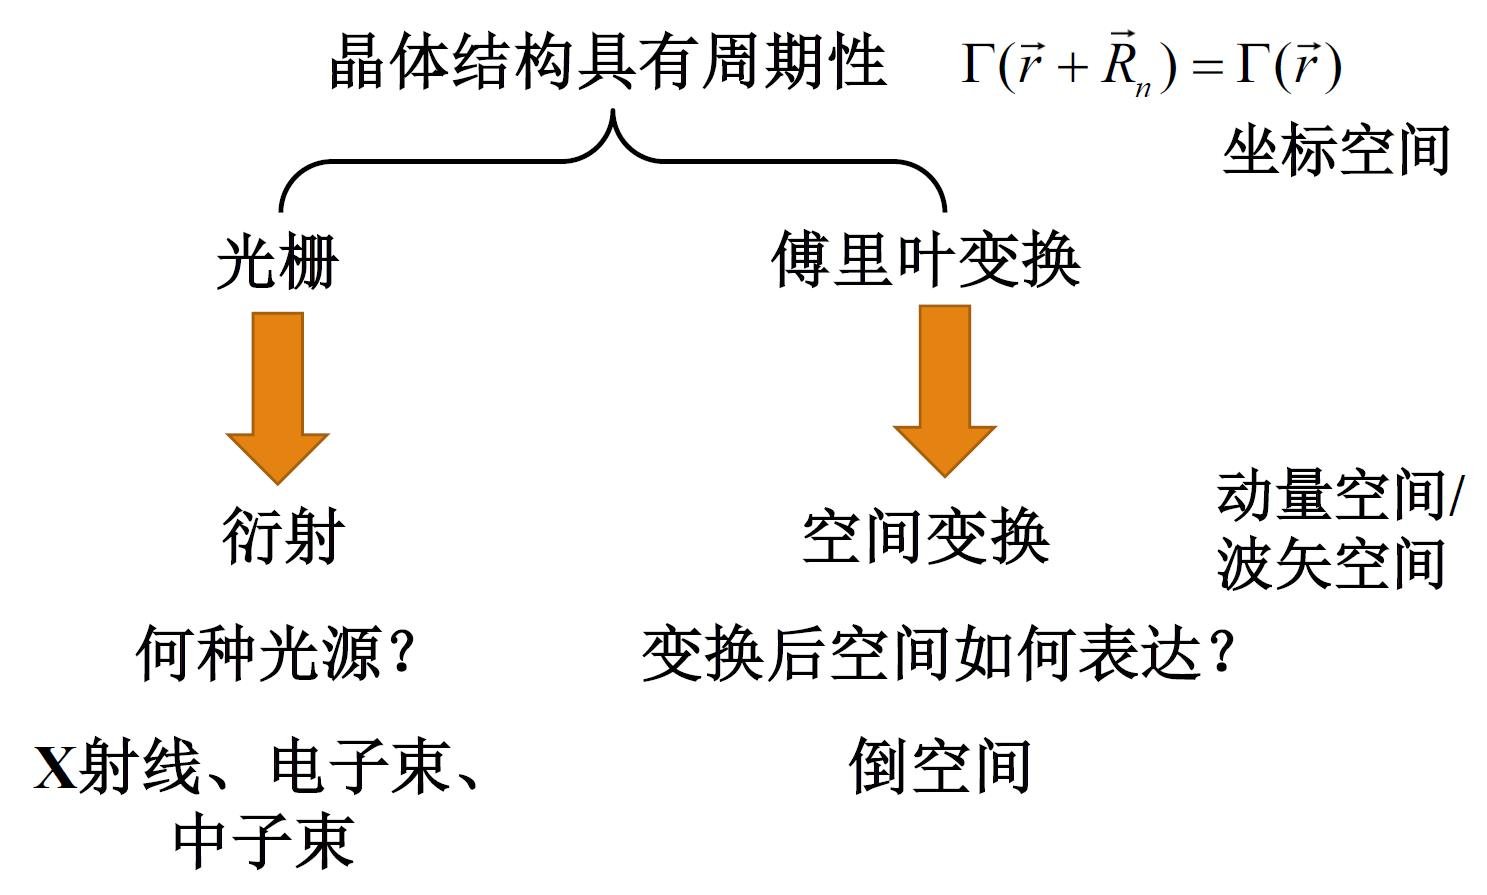
\includegraphics[width=0.9\textwidth]{figure/倒格子与布里渊区提纲.jpg}
        \caption{本章的基本内容与逻辑}
        \label{fig:CH3Index}
    \end{figure}
    
    本节我们考虑如何建立实验上分析晶体结构的方法。由于实验手段的限制,因此我们难以采用直接放大的方法测量固体的具体结构,我们往往采用电磁波与物质相互作用的方法进行测量。因此基于晶体的周期性排列,我们将晶体看作光栅,利用衍射的方法测量晶体。那么测量晶体需要什么光源呢?
    \begin{figure}[H]
        \centering
        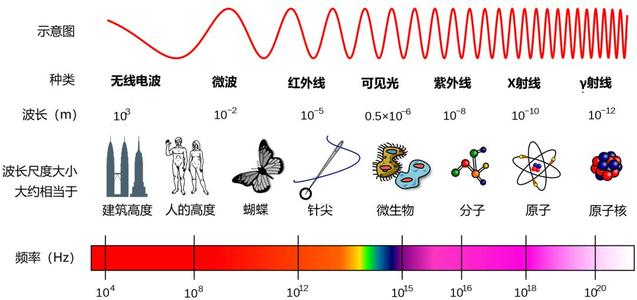
\includegraphics[width=0.7\textwidth]{figure/电磁波谱.jpeg}
        \caption{电磁波谱}
        \label{fig:electromagneticspectrum}
    \end{figure}
    
    根据光学的知识,我们知道只有当光的波长数量级与光栅常数d的数量级相似时,物体才会发生衍射现象。因此测量晶体所需要的电磁波的波长应该与这里的光栅常数——原子的半径数量级相似(可以参考图\ref{fig:electromagneticspectrum}),也即:
    
    \begin{equation}
        \lambda\sim 10^{-9}m
    \end{equation}
    
    对照电磁波谱的波长表,我们可以判断应该使用X射线来对晶体进行衍射实验。同时,我们也可以利用实物粒子(比如电子,中子)进行衍射,其波长满足De Brogile关系:
    \begin{equation}
        \lambda=\frac{h}{p}
    \end{equation}
    
    在之前的内容中,我们反复提及了晶体结构的核心概念就是平移对称性。这里的平移对称性不仅包括布拉维格子格点的平移对称性,同时晶体的其他性质,比如质量密度、电子云密度等都是具有平移对称性的,不失一般性,我们可以将平移对称性写成两个函数的等式:
    \begin{equation}\label{periodic}
        \Gamma(\Vec{r})=\Gamma(\Vec{r}+\Vec{R_n})
    \end{equation}
    
    其中函数$\Gamma$代表晶体的各种性质,$\Vec{R_n}$代表晶格平移矢量。在数学上,对于周期性体系,我们往往采用傅里叶级数展开的形式分析,对\eqref{periodic}式进行傅里叶级数展开,可得:
    \begin{align}
        \begin{split}
            \Gamma(\Vec{r})=&\sum_h \Gamma(\Vec{K_h})e^{i\Vec{K_h}\cdot \Vec{r}}\\
            \Gamma(\Vec{r}+\Vec{R_n})=&\sum_h \Gamma(\Vec{K_h})e^{i\Vec{K_h}\cdot (\Vec{r}+\Vec{R_n})}
        \end{split}
    \end{align}
    
    要\eqref{periodic}式成立,必须满足每一项相等,因此:
    \begin{equation}
        e^{i\Vec{K_h}\cdot \Vec{r}}=e^{i\Vec{K_h}\cdot (\Vec{r}+\Vec{R_n})}\Rightarrow e^{i\Vec{K_h}\cdot\Vec{R_n}}=1
    \end{equation}
    
    因此e指数一定满足周期性条件:
    \begin{equation}\label{periodicB}
        \Vec{K_h}\cdot \Vec{R_n} =2\pi m \quad m\in \mathbb{Z}
    \end{equation}
    
    同时,我们考虑格点的平移对称性,我们可以知道,体积V内$\Vec{R_n}$处的格点密度贡献为$\delta(\Vec{r}-\Vec{R_n})$,而在格点外的其它地方贡献为0,并且我们知道$\delta$函数满足全空间上的归一性:
    \begin{equation}
        \int \delta(\Vec{r}-\Vec{R_n}) d\Vec{r}=1
    \end{equation}
    
    因此如果体系中有N个格点,那么总的格点密度就可以表示为:
    \begin{equation}
        \rho(\Vec{r})=\sum_{\Vec{R_n}\in V}\delta(\Vec{r}-\Vec{R_n})
    \end{equation}

    对上式进行傅里叶分析,位于动量空间的展开系数可以表示为:
    \begin{align}
        \begin{split}
            \rho(\Vec{k})=&\int \rho(\Vec{r})e^{-i\Vec{k}\cdot\Vec{r}} d\Vec{r}\\
            =& \sum_{\vec{R_n}}\int \delta(\Vec{r}-\Vec{R_n})e^{-i\Vec{k}\cdot\Vec{r}} d\Vec{r}\\
            =&\sum_{\vec{R_n}} e^{-i\vec{k}\cdot \vec{R_n}}\\
            =&\sum_{\vec{R_n}} e^{-i(\vec{k}-\vec{K_h})\cdot \vec{R_n}}\\
           =&\sum_{\vec{K_h}}\delta(\vec{k}-\vec{K_h})
        \end{split}
    \end{align}
        
        其中倒数第二个式子利用了已经证明的关系$\vec{K_h}\cdot\vec{R_n}=2\pi m$;而最后一个等号利用了傅里叶变换中的Poisson求和公式。对比位移空间的布拉维格子的格矢密度和上式的形式,我们可以发现两个式子的形式是相同的。如此我们认为动量空间矢量$\vec{K_h}$端点构成的集合同样构成布拉维格子,称为倒格子。

        现在我们讨论倒格子基矢的性质,我们可以分别利用位移空间的基矢和动量空间的基矢对位移空间平移矢量$\vec{R_n}$和动量空间平移矢量$\vec{K_h}$进行展开:
        \begin{align}
            \begin{split}
                \vec{R_n}=&n_1\vec{a_1}+n_2\vec{a_2}+n_3\vec{a_3}\\
                \vec{K_h}=&h_1\vec{b_1}+h_2\vec{b_2}+h_3\vec{b_3}
            \end{split}
        \end{align}
        
        根据\eqref{periodic}式的周期性规律:$\vec{R_n}\cdot\vec{K_h}=2\pi m$,为了满足上述关系,我们可以得到正格子基矢$\vec{a_i}$和倒格子基矢$\vec{b_i}$的关系:
        \begin{equation}
            \vec{a_i}\cdot \vec{b_j}=\delta_{ij}
        \end{equation}
        
        上式说明$\vec{a_1}$和$\vec{b_1}$是共线的,换句话说$\vec{b_1}$和$\vec{a_2}\times\vec{a_3}$的方向是一样的,因此我们就有关系:
        \begin{equation}
            \vec{b_1}=\eta(\vec{a_2}\times\vec{a_3})
        \end{equation}
        
        由于$\vec{a_1}\cdot\vec{b_1}=2\pi$,所以:
        \begin{equation}
            \eta=\frac{2\pi}{\vec{a_1}\cdot(\vec{a_2}\times\vec{a_3})}=\frac{2\pi}{\Omega}
        \end{equation}
        
        其中$\Omega$是正格子原胞的体积。由此,我们可以得到倒格子基矢的另一种表述:
        \begin{align}
            \begin{split}
                \vec{b_1}=&\frac{2\pi}{\Omega}(\vec{a_2}\times\vec{a_3})\\
                \vec{b_2}=&\frac{2\pi}{\Omega}(\vec{a_3}\times\vec{a_1})\\
                \vec{b_3}=&\frac{2\pi}{\Omega}(\vec{a_1}\times\vec{a_2})\\
            \end{split}
        \end{align}
        
        倒格子和正格子之间还有一些关系:
        \begin{enumerate}
            \item 正格子和倒格子互为倒正关系
            \item 正格子原胞的体积$\Omega$与倒格子原胞体积$\Omega^*$满足以下关系:
                \begin{equation}
                    \Omega^*=\frac{(2\pi)^3}{\Omega}
                \end{equation}
            \item 正格子的晶面族($h_1,h_2,h_3$)与倒格矢$\vec{K_h}=h_1\vec{b_1}+h_2\vec{b_2}+h_3\vec{b_3}$,并且倒格矢的长度为$\frac{2\pi}{d_{h_1h_2h_3}}$,其中$d_{h_1h_2h_3}$是晶面族$(h_1,h_2,h_3)$的面间距。
            \item 面心立方和体心立方互为倒正关系。证明如下:
            
            面心立方的原胞矢量可以表示为:
            \begin{align}
                \begin{split}
                    \vec{a_1}=&\frac{a}{2}(\vec{i}+\vec{j})\\
                    \vec{a_2}=&\frac{a}{2}(\vec{i}+\vec{k})\\
                    \vec{a_3}=&\frac{a}{2}(\vec{j}+\vec{k})
                \end{split}
            \end{align}
            
            根据倒格矢的定义:
            \begin{align}
                \begin{split}
                    \vec{b_1}=&\frac{2\pi}{\Omega}(\vec{a_2}\times \vec{a_3})\\
                    =&\frac{8\pi}{a^3}\begin{vmatrix}
                    \vec{i} & \vec{j} & \vec{j}\\
                    \frac{a}{2} & 0 & \frac{a}{2}\\
                    0 & \frac{a}{2} & \frac{a}{2} \\
                    \end{vmatrix}\\
                    =& \frac{8\pi}{a^3}\frac{a^2}{4}(\vec{i}+\vec{j}-\vec{k})\\
                    =&\frac{2\pi}{a}(\vec{i}+\vec{j}-\vec{k})
                \end{split}
            \end{align}

            同理可以得到其它原胞基矢,由上式我们可以知道:面心立方结构的倒格子是边长为$\frac{4\pi}{a}$的体心立方。
        \end{enumerate}
        
        最后我们可以将正格子和倒格子的关系总结为图\ref{fig:recipricallattice}:
        \begin{figure}[H]
            \centering
            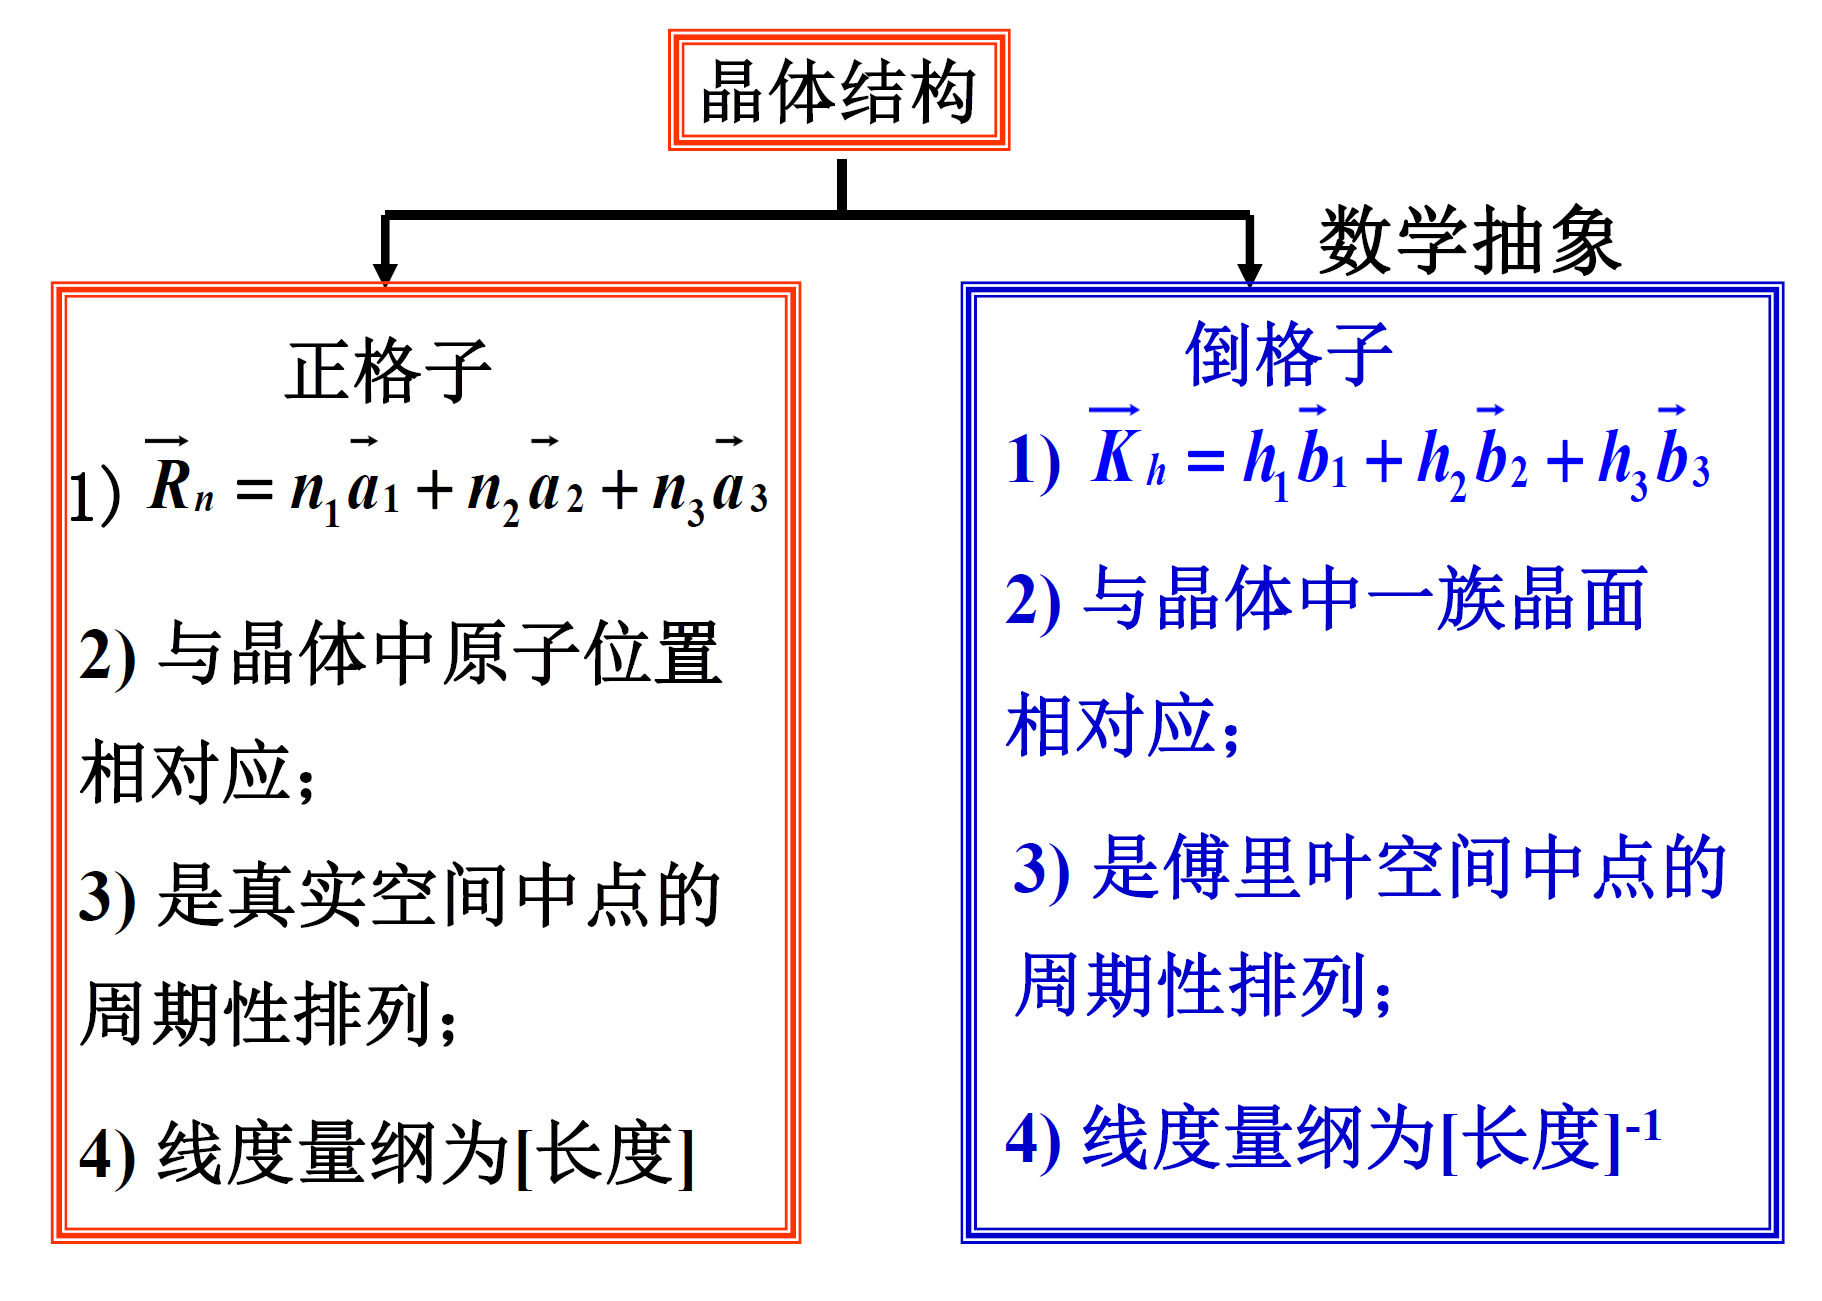
\includegraphics[width=0.9\textwidth]{figure/recipricallattice.png}
            \caption{正格子和倒格子的关系}
            \label{fig:recipricallattice}
        \end{figure}
        
        \subsection{布里渊区}
        上一节中,我们说明了倒格子也是Bravais格子,也有对应的倒空间原胞,于是,为了规范原胞的构造方法,我们同样可以定义倒空间中的W-S原胞。我们称倒空间中的W-S原胞为第一布里渊区。
        
        根据W-S原胞的定义,我们可以给出布里渊区的准确定义:任取一个倒格点为原点,作所有倒格矢$\vec{K_h}$的垂直平分面(又称布拉格面),这些平分面之间围成的区域称为布里渊区。进一步的,我们可以定义第n布里渊区的概念:
        \begin{itemize}
            \item 第一布里渊区:垂直平分面所围成的封闭的包含原点的最小空间(即倒空间的W-S原胞);
            \item 第二布里渊区:从第一布里渊区出发只穿过一个垂直平分面就可以到达的点的集合;
            \item 第n布里渊区:从第n-1个布里渊区出发只穿过一个垂直平分面就可以到达的点的集合。
        \end{itemize}
        
        我们通过两个例子熟悉布里渊区的基本概念和基本性质:
        
        首先考虑一维晶格的倒格子。假设正格子的晶格常数为a,则可以知道,倒格子的晶格常数为$\frac{2\pi}{a}$,根据定义,第一布里渊区的范围为$(-\frac{\pi}{a},\frac{\pi}{a}]$;第二布里渊区的范围为:$(-\frac{2\pi}{a},-\frac{\pi}{a}]\cup[\frac{\pi}{a}\cup\frac{2\pi}{a})$,具体如图\ref{fig:1DBrillouinzone}
        \begin{figure}[H]
            \centering
            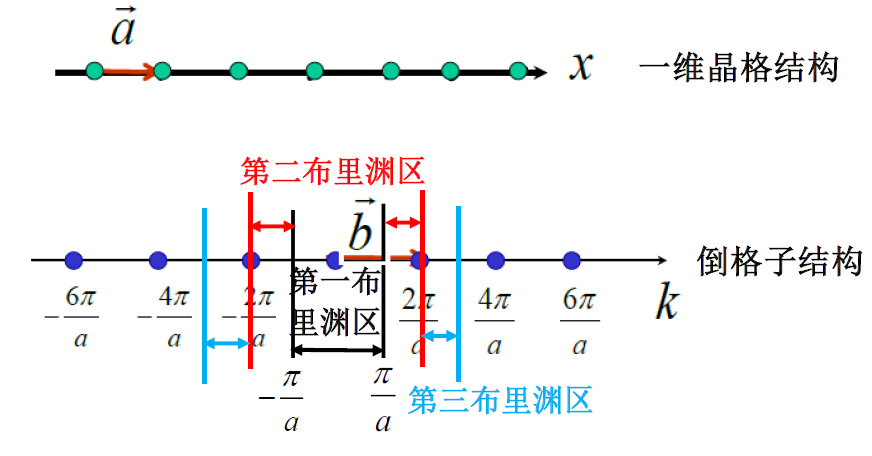
\includegraphics[width=0.9\textwidth]{figure/一维布里渊区.png}
            \caption{一维晶格的布里渊区示意图}
            \label{fig:1DBrillouinzone}
        \end{figure}
        同理我们可以考虑二维正方晶格的布里渊区,如图\ref{fig:2DBrillouinzone},我们可以发现一个重要结论:\textbf{每个布里渊区的体积(面积)都是相等的}。这个结论同样能够推广到三维。
        \begin{figure}[H]
            \centering
            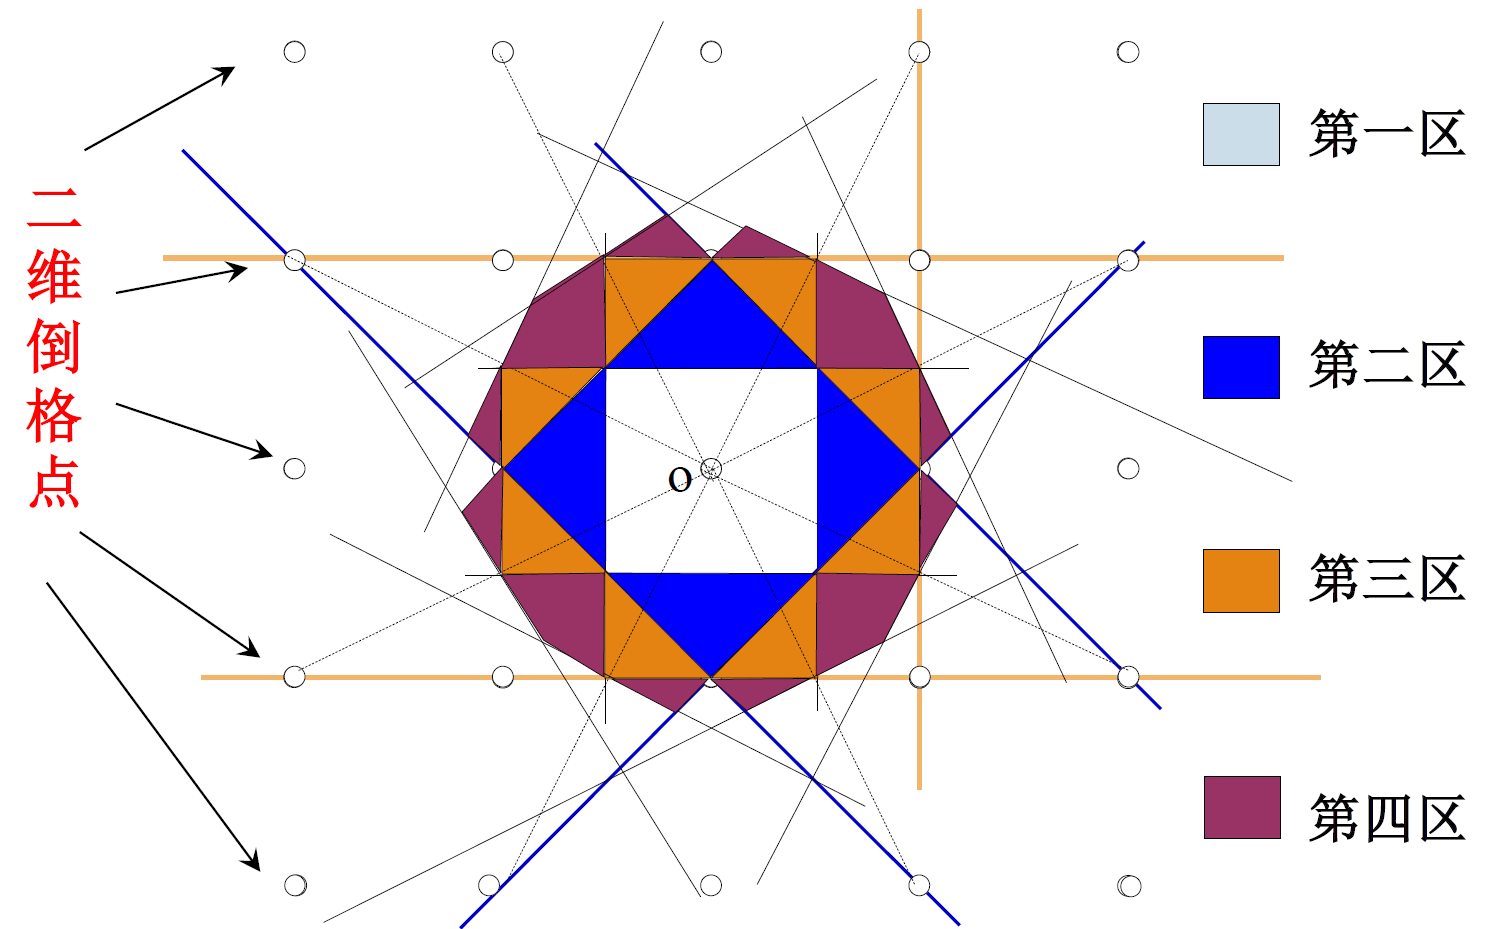
\includegraphics[width=0.9\textwidth]{figure/二维布里渊区.png}
            \caption{二维正方晶格的布里渊区示意图}
            \label{fig:2DBrillouinzone}
        \end{figure}
        
        
        \subsection{晶体的衍射条件}
        本章的开头讲过,晶体由于其周期性,可以视作衍射光栅。对于衍射问题,我们需要讨论两点:衍射极大与衍射相消处的条件和衍射强度。当观察点到晶体的距离,以及光源到晶体的距离比晶体尺寸大得多的时候,入射光和被观测的样射光都可以视为平行光线,我们从简单晶格出发,讨论晶体衍射的问题。
        
        \begin{figure}[H]
            \centering
            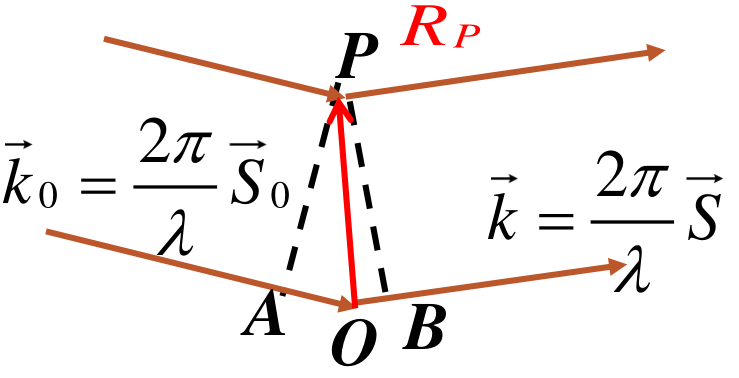
\includegraphics[width=0.6\textwidth]{figure/晶体衍射.png}
            \caption{X射线衍射}
            \label{fig:crystaldiffraction}
        \end{figure}
        
        其中$\vec{S_0}$和$\vec{S}$是入射线和衍射线的单位矢量,经过O格点和经过P格点的X光,衍射前后的光程差为:
        \begin{equation}
            AO+OB=-\vec{R_P}\cdot \vec{S_0}+\vec{R_p}\cdot \vec{S}=\vec{R_P}\cdot(\vec{S}-\vec{S_0})
        \end{equation}
        
        当X光是单色光,衍射加强的条件为:
        \begin{equation}
            \vec{R_P}\cdot(\vec{S}-\vec{S_0})=m\lambda,m\in\mathbb{Z}
        \end{equation}
        
        引入矢量$\vec{k}=\frac{2\pi}{\lambda}\vec{S}$,$\vec{k_0}=\frac{2\pi}{\lambda}\vec{S_0}$,上式可以改写为:
        \begin{equation}
            \vec{R_P}\cdot(\vec{k}-\vec{k_0})=2\pi m,m\in\mathbb{Z}
        \end{equation}
        
        根据量纲分析,我们可以知道$\vec{k}$的量纲是$[L]^{-1}$,同时对比倒格矢的定义式$\vec{R_P}\cdot\vec{K_h}=2\pi m$,因此我们可以将$\vec{k}$看做倒空间上的矢量,并且我们可以认为$\vec{k}-\vec{k_0}$一定是倒空间的某个平移矢量:
        \begin{equation}
            \vec{k}-\vec{k_0}=\vec{K_{h'}}
        \end{equation}
        
        并且该矢量与晶格倒空间的最短平移矢量$\vec{K_h}$之间一定存在倍数关系:
        \begin{equation}
            \vec{K_{h'}}=h'_1\vec{b_1}+h'_2\vec{b_2}+h'_3\vec{b_3}=n(h_1\vec{b_1}+h_2\vec{b_2}+h_3\vec{b_3})=n\vec{K_h}
        \end{equation}
        
        如此,衍射加强的条件又可以写作:
        \begin{equation}
            \vec{k}-\vec{k_0}=n\vec{K_h}
        \end{equation}
        
        其中n为整数,$(h'_1,h'_2,h'_3)$被称为衍射面指数,$(h_1,h_2,h_3)$是晶面指数。上式的几何意义如图\ref{fig:Braggequation}:如果忽略康普顿散射,则$|\vec{k}|=|\vec{k_0}|$,如果过$\vec{k}$的末尾做$n\vec{K_h}$的垂线,该垂线所在平面是$n\vec{K_h}$的中垂面。我们知道,晶面$(h_1,h_2,h_3)$与$\vec{K_h}$垂直,因此,该中垂面与晶面$(h_1,h_2,h_3)$平行,这个时候衍射极大的方向正好是晶面反射的方向。因此我们可以得到一个简单的结论:当衍射线对某一晶面族来说恰好是光的反射方向时,此衍射方向就是衍射加强的方向,我们可以看到某个晶体的X射线衍射图(见图\ref{fig:exampleXraydiffraction}),亮斑出现的地方就是衍射极大处。
        
        \begin{figure}[H]
            \centering
            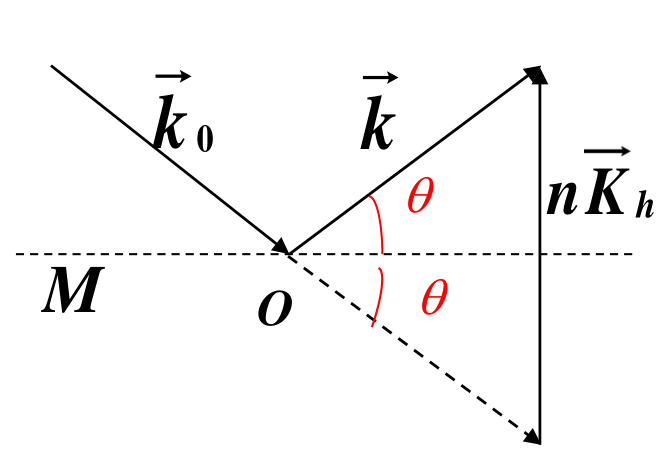
\includegraphics[width=0.6\textwidth]{figure/布拉格方程.png}
            \caption{$\vec{k}-\vec{k_0}$=n$\vec{K_h}$的示意图}
            \label{fig:Braggequation}
        \end{figure}
        
        \begin{figure}[H]
            \centering
            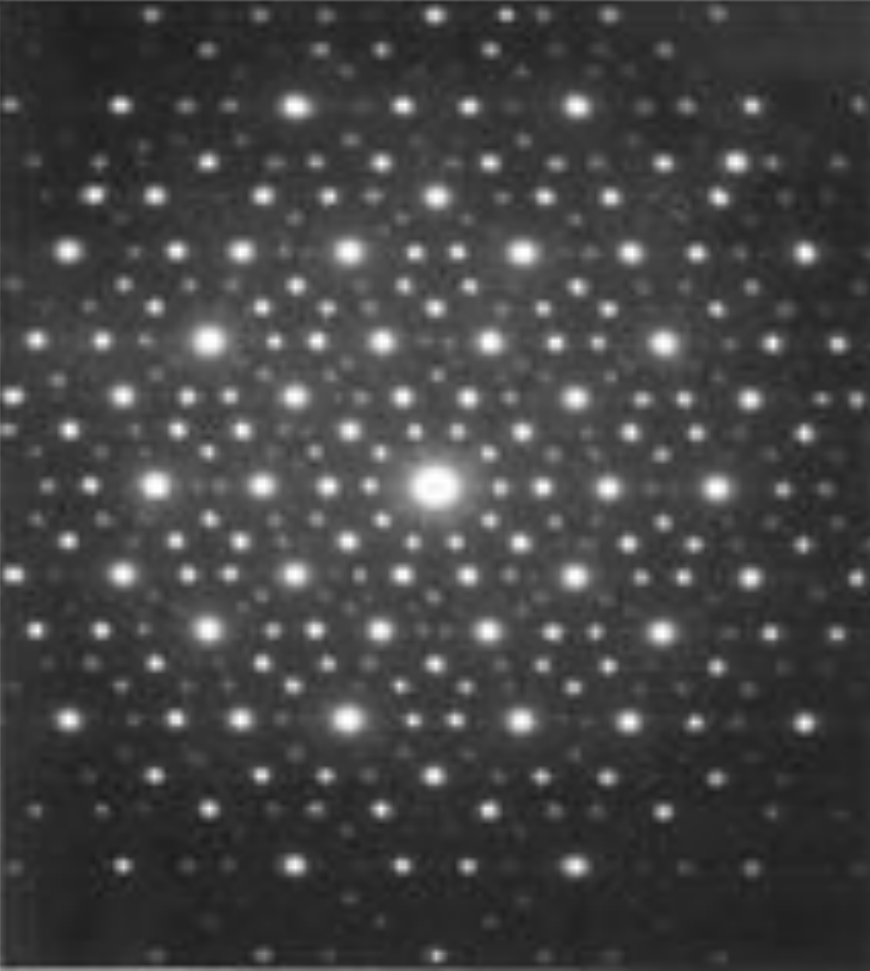
\includegraphics[width=0.4\textwidth]{figure/某晶体X射线衍射图.png}
            \caption{某晶体X射线衍射图}
            \label{fig:exampleXraydiffraction}
        \end{figure}
        
        由图\ref{fig:Braggequation},我们可以得到:
        \begin{equation}
            |\vec{k}-\vec{k_0}|=|n\vec{K_h}|=2\sin{\theta}|\vec{k}|=\frac{4\pi}{\lambda}
        \end{equation}
        
        又因为面间距$d_{h_1,h_2,h_3}=\frac{2\pi}{|K_{h'}|}$,于是上式可以继续化简为:
        \begin{equation}
            2d_{h_1,h_2,h_3}\sin{\theta}=n\lambda
        \end{equation}
        
        该式被称为Bragg方程,根据下图(图\ref{fig:Braggreflection}),我们可以看到该方程的几何意义。
        
        \begin{figure}[H]
            \centering
            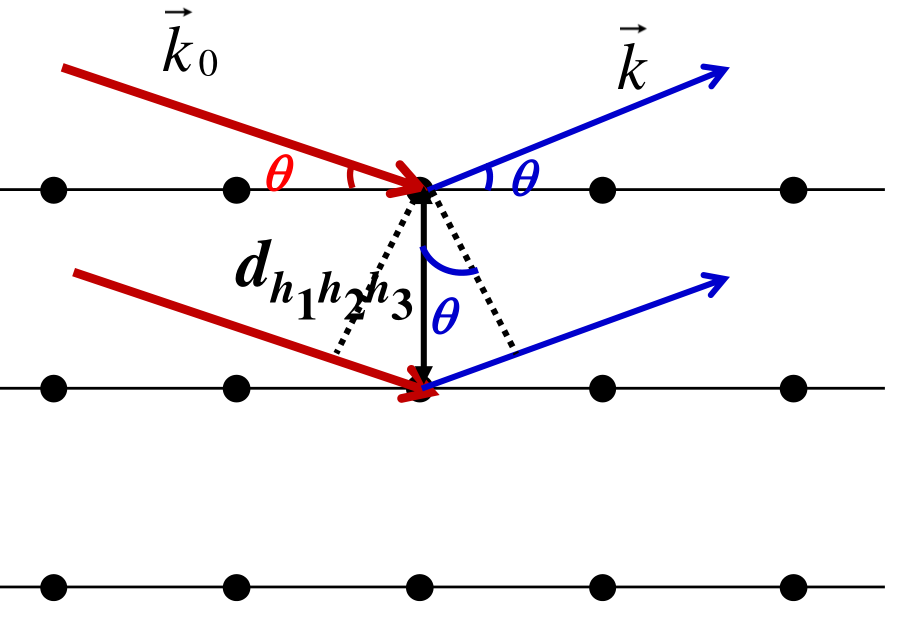
\includegraphics[width=0.5\textwidth]{figure/布拉格反射.png}
            \caption{布拉格反射}
            \label{fig:Braggreflection}
        \end{figure}
        
        上面我们已经得到了X射线对于晶胞的衍射关系,下面我们要详细探讨晶胞内原子及其排列对衍射强度及其分布的关系。我们采用的说明顺序是有小至大,从一个原子的电子受到散射到原子之间的电子散射波相互干涉最后到晶胞内原子的衍射,分别对应一个散射因子,框架可以见下图(图\ref{fig:diffractionintensity})
        \begin{figure}[H]
            \centering
            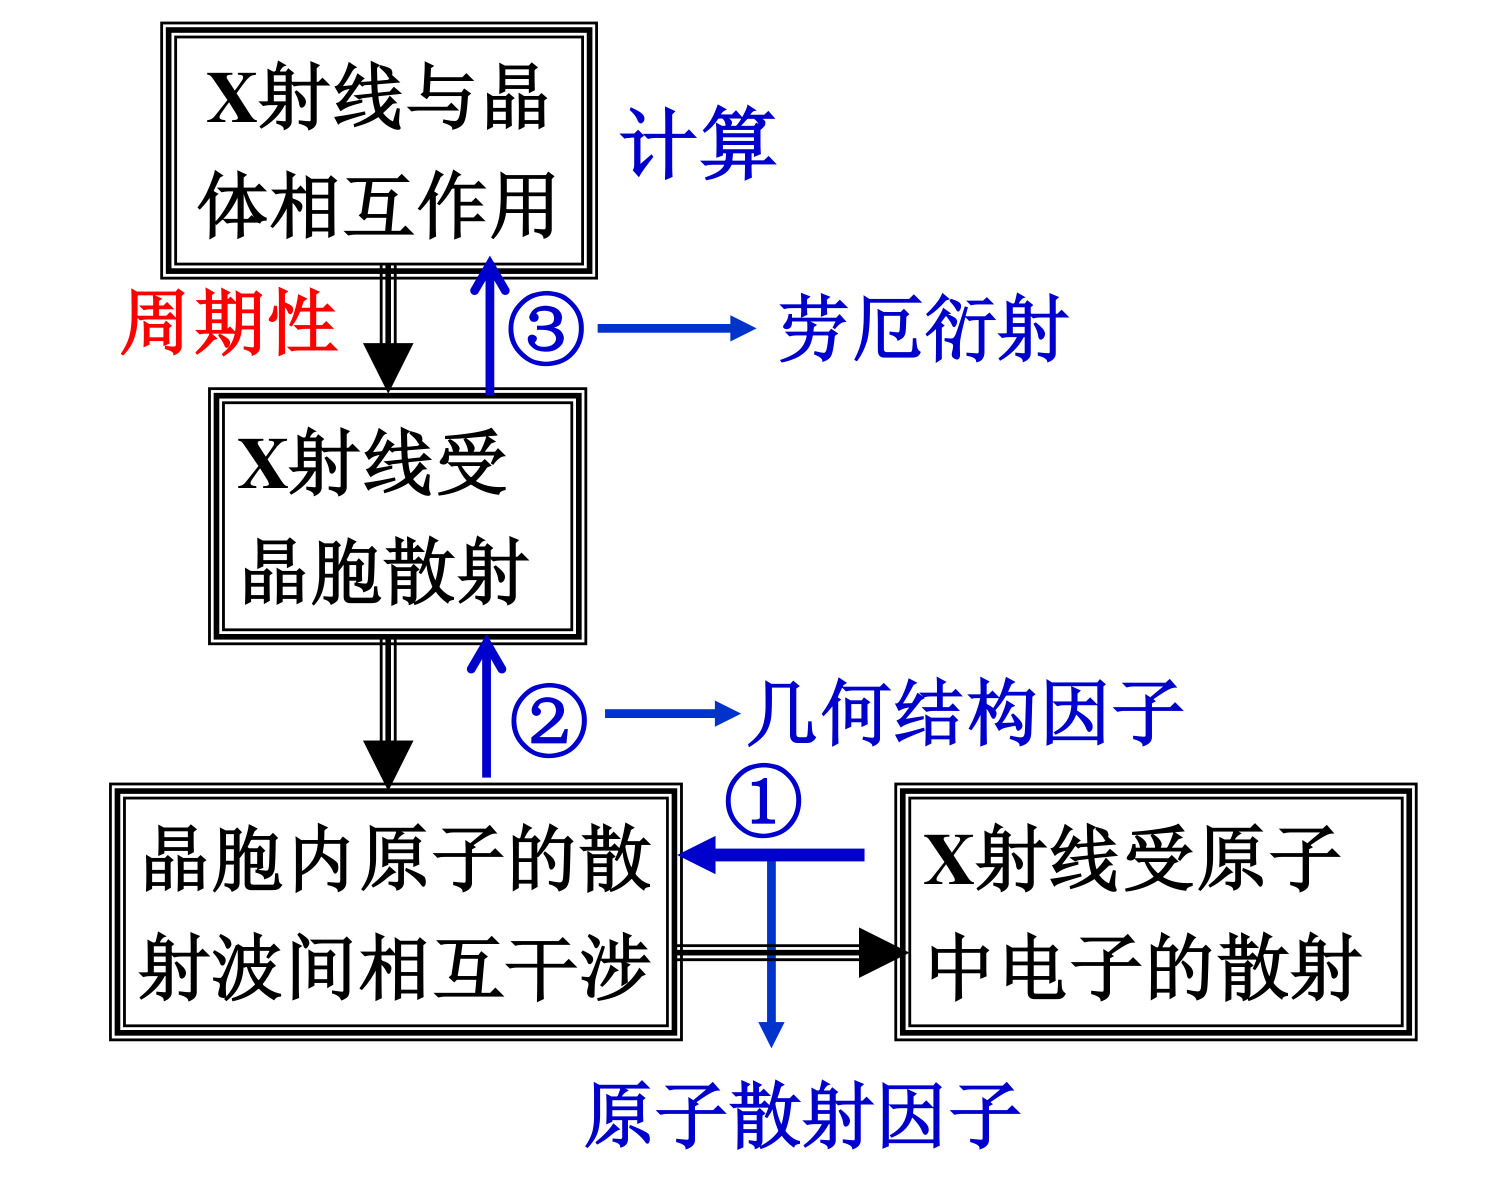
\includegraphics[width=0.4\textwidth]{figure/衍射强度.png}
            \caption{衍射强度研究框架}
            \label{fig:diffractionintensity}
        \end{figure}
        
        原子对X光的散射,本质上是原子内的电子对X光的散射,而原子内的电子云分布不同,原子对X光的散射特性不同,我们将这个现象总结为原子散射因子不同。
        
        原子散射因子的定义是原子所有电子在某一方向上引起的散射波的振幅之矢量和与某一个电子在该方向上引起的散射波的振幅之比。根据该定义,我们可以知道f的含义是原子在某一方向上的振幅是单个电子在该方向上振幅的倍数,表现了原子在这个方向上的散射效率。
        下面探讨X射线在原子中散射的具体形式。如下图(图\ref{fig:diffractioninatom}),设$\vec{r}$是P点的位矢,入射光和反射光的单位矢量分别为$\vec{S_0},\vec{S}$,则原子中心与P点的散射波的相位差为:
        \begin{equation}
            \varphi=\frac{2\pi}{\lambda}(\vec{S}-\vec{S_0})\cdot=(\vec{k}-\vec{k_0})\cdot \vec{r}
        \end{equation}
        \begin{figure}[H]
            \centering
            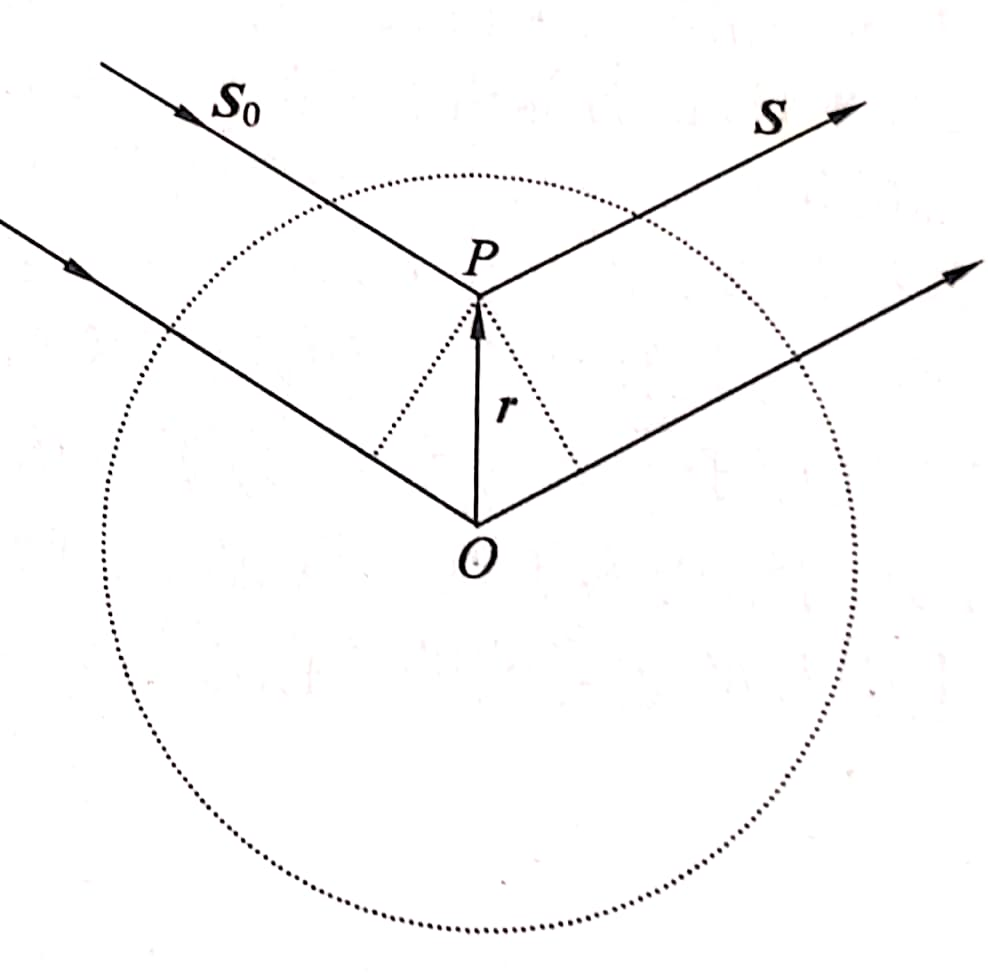
\includegraphics[width=0.5\textwidth]{figure/X射线在原子中的散射.jpg}
            \caption{X射线在原子中的散射}
            \label{fig:diffractioninatom}
        \end{figure}
        
        设想,原子中心处一个电子在$\vec{S}$方向处引起的散射波在观察点的振幅为A,则P点处电子在$\vec{S}$方向处引起的散射波在观察点的振幅为:
        \begin{equation}
            A\exp{[-i(\vec{k}-\vec{k_0})\cdot \vec{r}]}
        \end{equation}
        
        于是,根据定义,我么可以得到原子散射因子:
        \begin{equation}
            f=\frac{\sum_{\vec{r_j}}A\exp{[-i(\vec{k}-\vec{k_0})\cdot \vec{r_j}]}}{A}=\sum_{\vec{r_j}}\exp{[-i(\vec{k}-\vec{k_0})\cdot \vec{r_j}]}
        \end{equation}
        
        离散的情况不利于我们实际上对其进行计算,我们往往会使用连续版本。设P点附近$d\tau$大小的体积元的概率密度为$\rho(\vec{r})$,则原子散射因子可以表示为:
        \begin{equation}
            f=\int \rho(\vec{r})\exp{[-i(\vec{k}-\vec{k_0})\cdot \vec{r}]}d\tau
        \end{equation}
        
        根据上式,我们可以知道:根据$\vec{k}-\vec{k_0}$,$\vec{k_0}$的方向一定,所以f依赖于散射方向$\vec{S}$;不同原子$\rho(\vec{r})$不同,因此原子散射因子也不同。
        
        对于不同原子组成的晶胞,要研究X光的衍射相对来说较为复杂,但是其核心也是不变的。核心在于两点:1、各个衍射极大的相位差;2、衍射的强度。前者依赖于各个晶格的相对距离,后者依赖于原子散射因子。为了概括这两个因素对X光衍射的影响,我们引入几何散射因子。其定义为:原胞内所有原子在某一方向上引起的散射波的总振幅与某一电子在该方向上所引起的散射波的振幅之比。
        
        设原胞内t个不同原子的相对位矢分别为:$\vec{r_1},\vec{r_2},\cdots,\vec{r_t}$,于是在坐标原点的原胞中,各个原子的散射振幅分别为$\Bar{A_1},\Bar{A_2}\cdots\Bar{A_t}$,其中:
        \begin{equation}
            \Bar{A_i}=f_iA\exp{[-i(\vec{k}-\vec{k_0})\cdot \vec{r_i}]}
        \end{equation}
        
        其中A是坐标原点的原子中心处一个电子在某一个方向上的散射振幅,根据几何散射因子的定义,我们可以知道:
        \begin{equation}
            F=\sum_j f_j \exp{[-i(\vec{k}-\vec{k_0})\cdot \vec{r_j}]}
        \end{equation}
        
        根据前面的说明,当$\vec{k}-\vec{k_0}=\vec{K_{h'}}=m\vec{K_h}$时,衍射极大。如果我们采用密勒指数,则是当(h',k',l')=m(h,k,l)时,出现衍射极大,此时几何散射因子就是$\vec{K_{(h',k',l')}}$的函数:
        \begin{equation}\label{equ:3geometricdiffractionfactor}
            F(\vec{K_{(h',k',l')}})=\sum_j f_j \exp{[-i\vec{K_{(h',k',l')}}\cdot \vec{r_j}]}
        \end{equation}
        
        如果我们用倒空间晶格矢量表示倒空间平移矢量,正空间晶格矢量表示相对位矢,即:
        \begin{align}
            \begin{split}
                \vec{K_{(h',k',l')}}=& h'\vec{b_1}+k'\vec{b_2}+l'\vec{b_3}\\
                \vec{r_j}=u_j\vec{a_1}+v_j\vec{a_2}+w_j\vec{a_3}
            \end{split}
        \end{align}

        代入\eqref{equ:3geometricdiffractionfactor}式,结合正空间晶格矢量与倒空间晶格矢量的关系$\vec{a_i}\cdot\vec{b_j}=2\pi r\delta_{ij},r\in \mathbb{Z}$,我们可以得到:
        \begin{equation}
             F_{h,k,l}=\sum_j f_j \exp{[-2i\pi m(hu_j+kv_j+lw_j)]}
        \end{equation}
        
        上式就可以表现原子的相对位置对散射的影响,因此(h,k,l)晶面族引起的衍射光的总强度为:
        \begin{equation}
            I_{h,k,l}\propto |F_{h,k,l}|^2=\{\sum_j f_j\cos{[2m\pi(hu_j+kv_j+lw_j)]}\}^2+\{\sum_j f_j\sin{[2m\pi(hu_j+kv_j+lw_j)]}\}^2
        \end{equation}
        
        特别的,如果$F_{(h,k,l)}=0$,此时衍射光斑消失,我们称为消光。下面我们简单看一下几个常见晶体结构的消光条件:
        \begin{itemize}
            \item 对于简单立方,晶胞内只有一个原子,坐标为(0,0,0),此时$I_{h,k,l}\propto |f_j|^2$,没有消光;
            \item 对于体心立方,晶胞内有两个原子,坐标为(0,0,0),$(\frac{1}{2},\frac{1}{2},\frac{1}{2})$,此时:
            \begin{equation}
                I_{h,k,l}\propto |\sum_j f_j(1+\cos{[\pi m(h+k+l)])}|^2
            \end{equation}
            
            可以发现,当$m(h+k+l)$为奇数时,产生消光。我们可以观察体心立方的Fe的衍射谱(见图\ref{fig:bccFediffraction}),产生衍射强度的地方$m(h+k+l)$都为偶数。
            \begin{figure}[H]
                \centering
                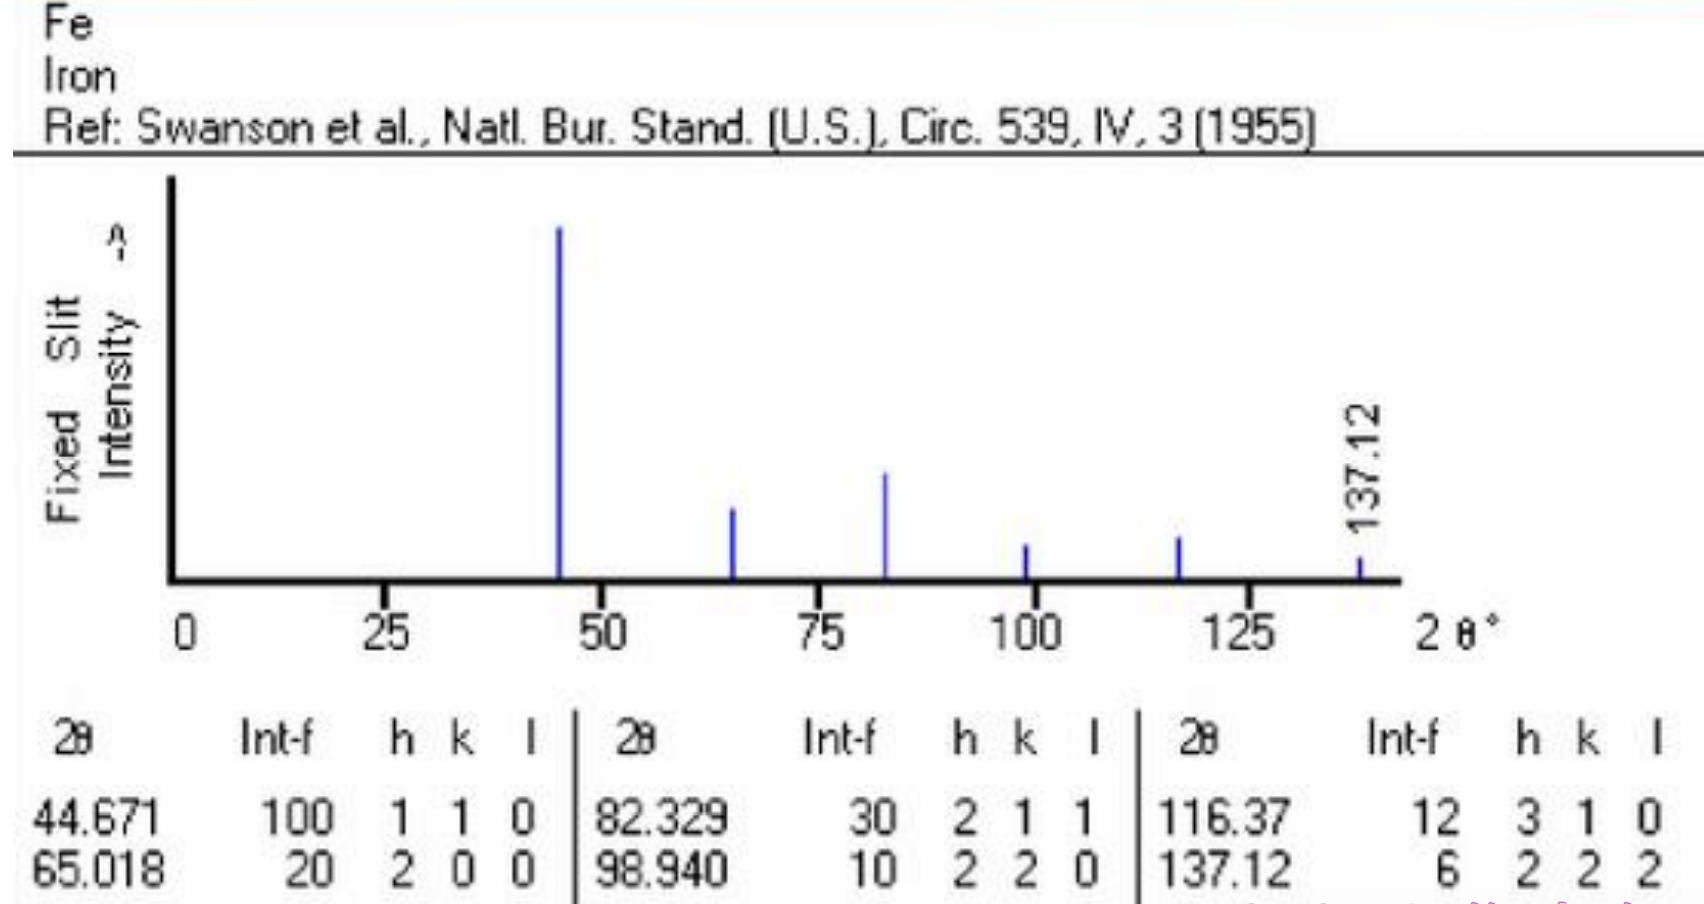
\includegraphics[width=0.9\textwidth]{figure/铁的衍射谱.png}
                \caption{体心立方Fe的衍射谱}
                \label{fig:bccFediffraction}
            \end{figure}
            \item 对于面心立方,晶胞内有四个原子,坐标为为(0,0,0),$(0,\frac{1}{2},\frac{1}{2}),(\frac{1}{2},0,\frac{1}{2})$,$(\frac{1}{2},\frac{1}{2},0)$,此时:
            \begin{equation}
                I_{h,k,l}\propto |\sum_j f_j(1+\cos{[\pi m(h+k)]+\cos{[\pi m(h+l)]}+\cos{[\pi m(k+l)]})}|^2
            \end{equation}
            
            可以发现,当$mh,mk,ml$不是同奇偶,会产生消光,我们可以观察面心立方的Fe的衍射谱来验证我们的发现(见图\ref{fig:fccFediffraction})
            \begin{figure}[H]
                \centering
                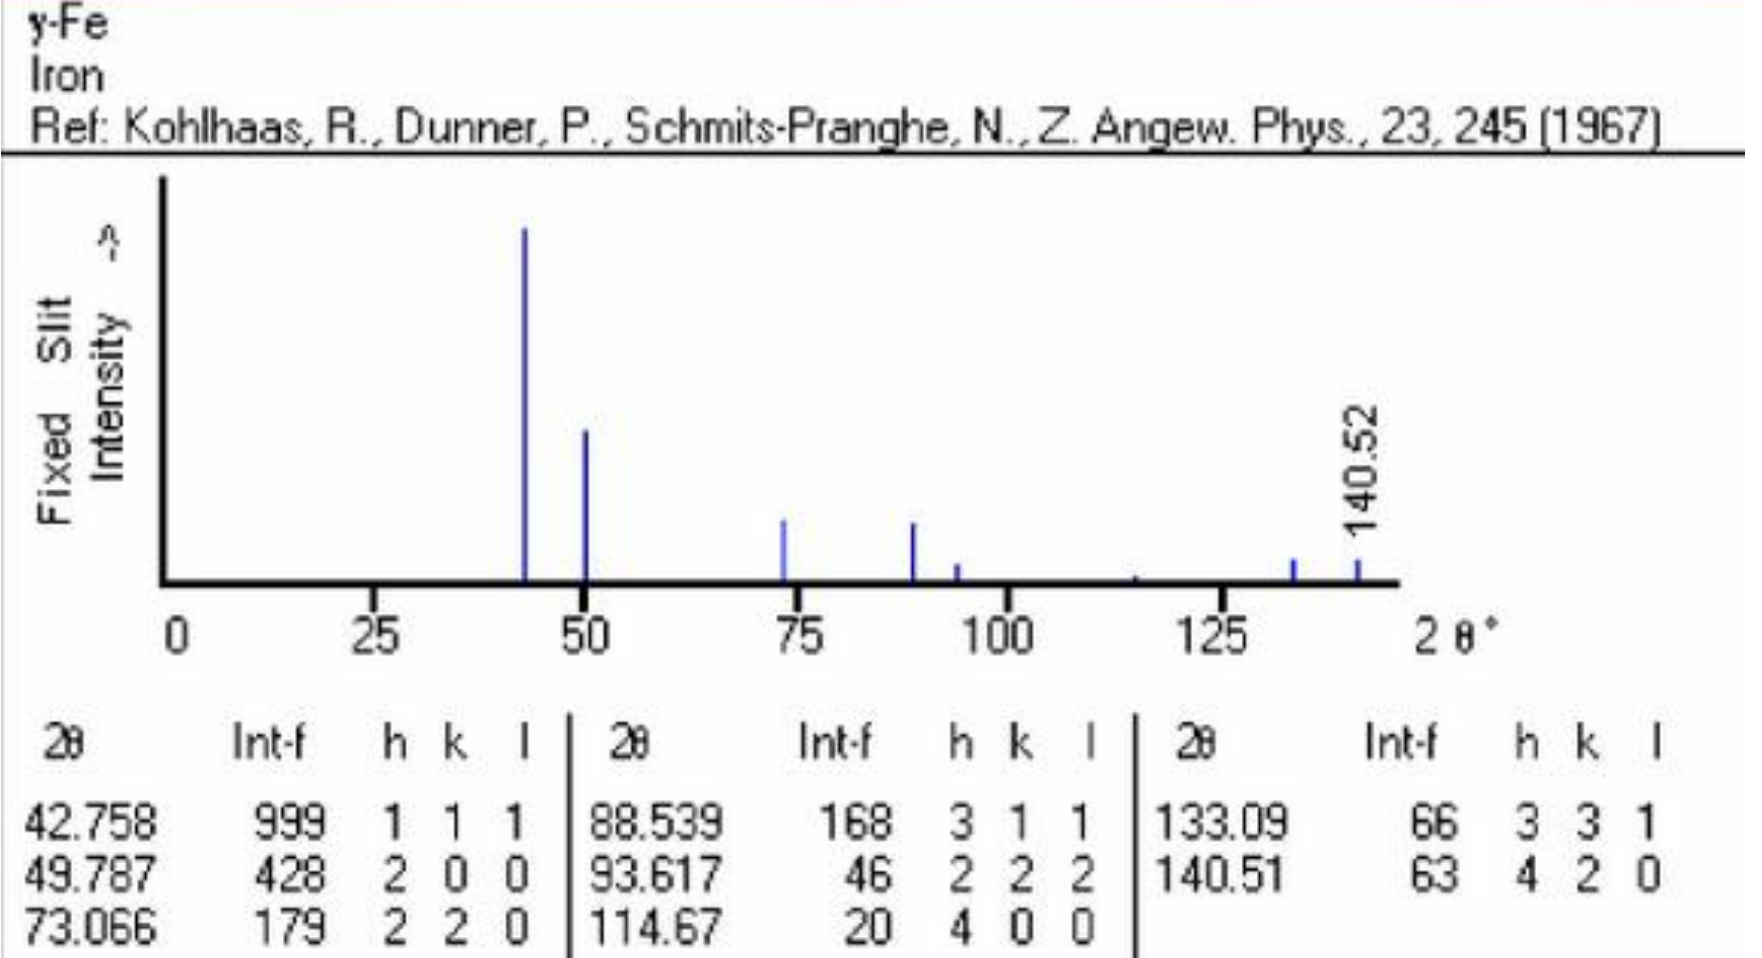
\includegraphics[width=0.9\textwidth]{figure/面心立方Fe的衍射谱.png}
                \caption{面心立方Fe的衍射谱}
                \label{fig:fccFediffraction}
            \end{figure}
        \end{itemize}
        \newpage
    \section{晶格的振动}
        \subsection{简介}
        上一章,我们主要考虑了固体静止时候几何结构对固体性质的影响。事实上,微观粒子每时每刻都在发生热运动,因此为了进一步的讨论固体的物理性质(如比热、热膨胀等)和微观变化,我们必须考虑所谓晶格的振动(即离子实的振动)。
        
        我们知道,对于固体体系,我们可以写出其Schrodinger方程:
        \begin{equation}
            \hat{H}\psi(\vec{r},\vec{R})=E\psi(\vec{r},\vec{R})
        \end{equation}
        
        其中$\vec{r}$表示电子的位矢,$\vec{R}$表示离子实的位矢,$E$是体系的总能量。同时总的Hamiltonian可以表示为:
        \begin{equation}
            \hat{H}=\hat{T_N}+\hat{T_e}+\hat{V_{MN}}(\vec{R})+\hat{V_{ij}}(\vec{r})+\hat{V_{iM}}(\vec{r},\vec{R})
        \end{equation}
        
        其中第一项表示离子实的动能,第二项表示电子的动能,第三项表示离子实之间的相互作用,第四项表示电子之间的相互作用,第五项表示核与电子的相互作用。通过B-O近似,我们可以将电子的运动与离子实的运动分开,这表现在波函数、Hamiltonian和能量上:\footnote{其推导和逻辑详见笔者量子化学的笔记}:
        \begin{align}
            \begin{split}
                \psi(\vec{r},\vec{R})=&\varphi(\vec{r})\chi(\vec{R})\\
                \hat{H}=&\hat{H_e}+\hat{H_N}\\
                E=&E_e+E_N
            \end{split}
        \end{align}
        
        我们可以证明,晶格的Schrodinger方程可以写成:
        \begin{equation}
            \hat{H_N}\chi(\vec{R})=E_N\chi(\vec{R})
        \end{equation}
            
        其中:
        \begin{align}
            \begin{split}
                \hat{H_N}=&\hat{T_n}+\hat{V}(\vec{R})\\
                \hat{V}(\vec{R})=\hat{V_{MN}}(\vec{R})+\int\psi^*(\vec{r},\vec{R_n}&)[\hat{V_{iN}}(\vec{r},\vec{R})-\hat{V_{iN}}(\vec{r},\vec{R_n})]\psi(\vec{r},\vec{R_n})d\vec{r}.
            \end{split}
        \end{align}
    
        可以看到,晶格的Schrodinger方程中的势能项不仅和晶格之间的相互作用有关,同时也和电子的作用有关。可以发现,求解该Schrodinger方程的困难在于粒子之间的作用相互耦合,形成一个多体问题,难以求解。由于晶格的振动可以被看作离子实在平衡位置附近的微小振动,因此我们可以通过将势能函数进行幂级数展开并忽略高阶项的方式对势能进行化简(我们称这种做法为\textbf{简谐近似},因为此时势能函数可以看作简谐振子的振动)。由于简谐近似下的微小振动作为经典力学问题有精确解,并且量子力学的处理仅仅是对经典力学运动模式下的能量进行了正则量子化。因此本章模型引入的主体逻辑是从简谐晶体的经典运动到量子力学处理,具体如下:
        \begin{itemize}
            \item 晶格振动的经典力学处理:通过从一维到三维;从单原子链到双原子链,逐步推广得到一般离子实的运动方程,同时根据运动方程,我们可以得到格波的概念和能量(频率)和波矢的关系(我们称之为色散关系$\omega(\vec{q})$)。
            \item 晶格振动的量子力学处理:我们采用的方法是遵循分析力学中的方法:引入简正坐标将多体问题单体化,将格波的能量转化为了求解引入了简正坐标后谐振子的能量。由此我们可以大大简化晶体势场$V(\vec{R})$的形式。不仅如此,为了更加形象的描述等效的谐振子能量,我们引入了一种准粒子——声子来描述晶格振动的能量子。
        \end{itemize}
        
        本章的最后会利用引入得晶格振动的模型解释固体的一些性质:比如固体的热学性质(本章讨论的重点是热容)还有格波与电磁波的耦合作用。最后我们通过讨论热膨胀和热传导引出非简谐项对模型的影响。
        \subsection{一维晶体振动}
            本节我们通过经典力学的方法,通过求解一维单原子链,一维双原子链的运动学方程,得到色散关系和格波的关系,然后通过格波的量子化得到格波的能量关系。
            \subsubsection{一维单原子链}   
            我们首先考虑一维单原子链(如图\ref{fig:1Dmonoatomic}),设原子的质量为m,晶格常数为a,晶胞数为N,第n个原子在t=0时刻与t时刻的位移之差为$u_n$。我们可以将势能函数$V(r)$在平衡位置$r=r_0$处进行泰勒展开:
            \begin{figure}[H]
                \centering
                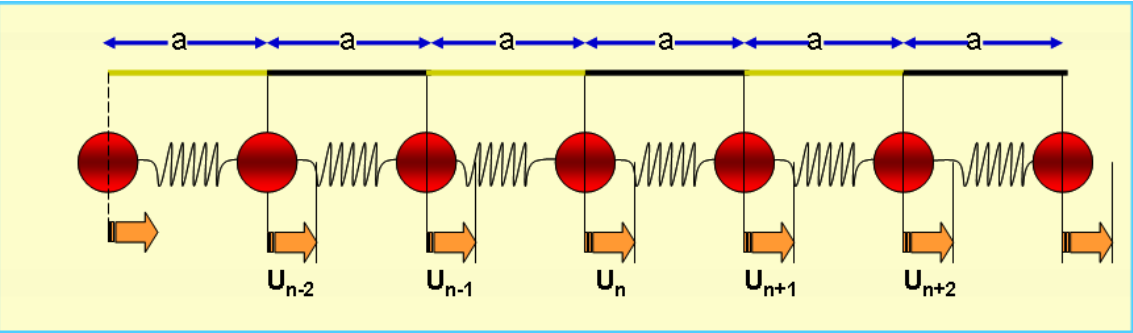
\includegraphics[width=0.8\textwidth]{figure/1Dmonoatomic.png}
                \caption{一维单原子链示意图}
                \label{fig:1Dmonoatomic}
            \end{figure}
            
            \begin{equation}
                V(r)=V(r_0)+\left.\frac{dV(r)}{dr}\right|_{r=r_0}\Delta r+\frac{1}{2!}\left.\frac{dV^2(r)}{dr^2}\right|_{r=r_0}(\Delta r)^2+\dots
            \end{equation}
            
            由于势能零点是任意的,因此我们可以令$V(r_0)=0$,同时,平衡处满足$V'(r_0)=0$,因此在忽略高阶项的情况下(这个思想就是简谐近似的思想,在后面我们会考虑高阶项,也就是非简谐的影响),原子振动的势能函数可以写成:
            \begin{equation}
                V(r)=\frac{1}{2}\beta (\Delta r)^2
            \end{equation}
            
            其中:
            \begin{equation}
                \beta=\left.\frac{dV^2(r)}{dr^2}\right|_{r=r_0}
            \end{equation}

            根据势能函数,我们可以求得势场产生的力为:
            \begin{equation}
                F=-\frac{dV}{dr}=-\beta\Delta r
            \end{equation}

            考察第n个原子所受的作用力,一方面,它等于其它所有原子对这个原子产生的作用力之和,而另一方面,这个作用力也可以简单地用牛顿第二定律表示,于是可以得到:
            \begin{equation}
                m\ddot{u_n}=F_n=-\sum_{k\ne n}\beta_{nk}\Delta r_{nk}
            \end{equation}
            
            其中根据定义我们可以很清楚的知道$\Delta r_{nk}=u_n-u_k$。由于其它所有原子对这个原子产生的总作用力形式还是非常的复杂,因此在这里,我们只考虑最近邻的两个原子(第n-1个原子和第n+1个原子)对这个原子的作用力(即所谓的\textbf{最近邻近似}),于是运动方程可以表达为:
            \begin{equation}\label{equ:motionequ}
                m\ddot{u_n}=-\beta(u_n-u_{n-1}+u_n-u_{n+1})=\beta(u_{n-1}+u_{n+1}-2u_n)
            \end{equation}
            
            由于有N个原胞,因此一维单原子链的运动实际上是一个互相耦合的N阶方程组。求解起来仍然十分困难,在这里,我们有一个非常讨巧的解法\footnote{说它讨巧的原因是:实际上我们已经默认原子的振动是按照波的形式进行传播的,有一点由果推因的感觉},就是给出平面波试探解:
            \begin{equation}
                u_n=A_q e^{i(kr_n-\omega t)}=A_q e^{i(k a n-\omega t)}
            \end{equation}
            
            代入运动方程(式\eqref{equ:motionequ})中,我们可以得到:
            \begin{equation}
                \omega=2\sqrt{\frac{\beta}{m}}|\sin{\frac{ka}{2}}|
            \end{equation}
            
            上式被称为一维单原子格波的色散关系。下面对专业术语进行分析:
            
            \begin{itemize}
                \item 根据试探解的形式我们知道,我们认为某个原子在平衡位置附近的振动以波的形式在晶体中传播,这是一种晶体中所有原子参与的集体运动,我们称之为格波(lattice wave)
                \item 为什么$\omega\sim k$的关系被叫做色散关系(dispertion relation)呢?色散关系的最初来源是牛顿发现光在介质中的传播速度(即所谓群速度)与光的频率有关,我们用折射率n来表示光在介质中的传播速度,那么可以得到$n\sim \nu$,我们将这种关系称作色散关系。可以发现折射率$n$与波速有关,而频率与波长有关,因此广义上,波速$\sim$波长和其衍生的对应关系都可以叫做色散关系。
            \end{itemize}
            
            随后我们讨论具体讨论一维单原子格波的色散关系,可以发现,这是一个以$\frac{2\pi}{a}$为周期的周期函数,即$\omega(k)=\omega(k+\frac{2\pi m}{a}),m\in \mathbb{Z}$,函数图像如图\ref{fig:dispersionrelation}:
            \begin{figure}[H]
                \centering
                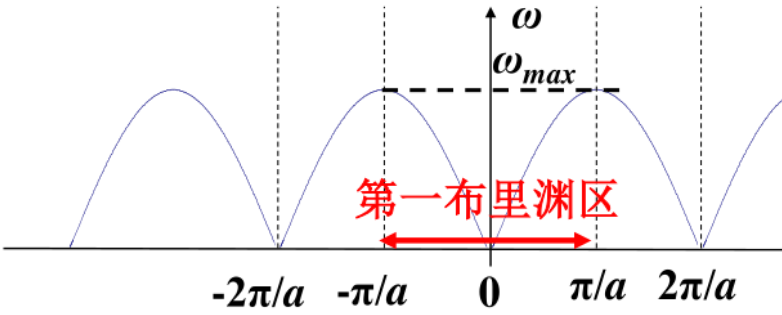
\includegraphics[width=0.6\textwidth]{figure/色散关系.png}
                \caption{色散关系曲线图}
                \label{fig:dispersionrelation}
            \end{figure}
            
            由于波矢空间中$\frac{2\pi}{a}$正好是倒格子的空间平移基矢$\vec{K_h}$的模长,因此我们可以得到结论:波矢相差$\vec{K_h}$的原子的运动方式是完全相同的。观察图\ref{fig:independentlatticewave}的例子,我们可以发现波长为$4a$和波长为$\frac{4}{5}a$的波上的原子的运动轨迹完全重合\footnote{ 这里就体现出格波与一般连续介质中波的不同了,虽然两者振动方程形式类似,但是连续介质波中的x表示空间内任意一点,而格波只取周期性排列的格点;同时格波表示所用原子的集体振动。}。
            \begin{figure}[H]
                \centering
                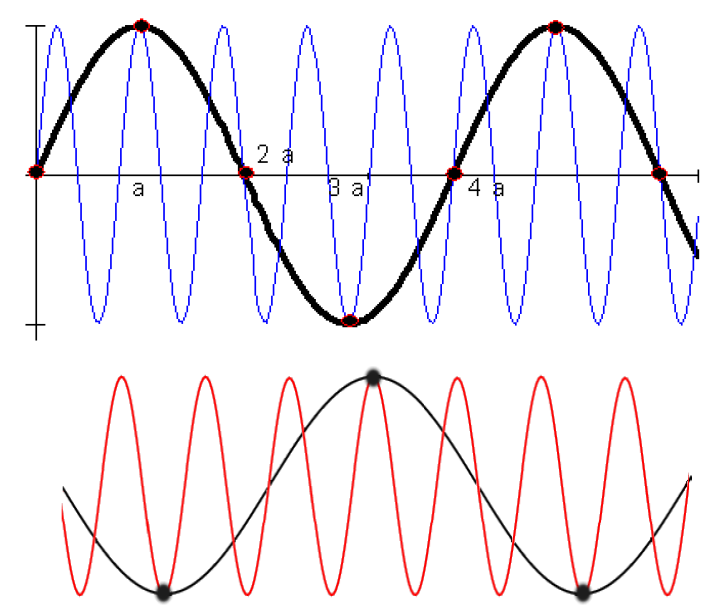
\includegraphics[width=0.6\textwidth]{figure/独立格波.png}
                \caption{波长为$4a$与$\frac{4}{5}a$的波(波矢相差$\frac{2\pi}{a}$),原子的运动方式完全相同}
                \label{fig:independentlatticewave}
            \end{figure}
            
           因此如果我们想要讨论格波的性质,只需要考虑第一布里渊区内的k即可(如图\ref{fig:dispertionrelationin1stBZ}),我们称第一布里渊区中满足要求的k对应的格波为独立格波(independent lattice wave)。
            \begin{figure}[H]
                \centering
                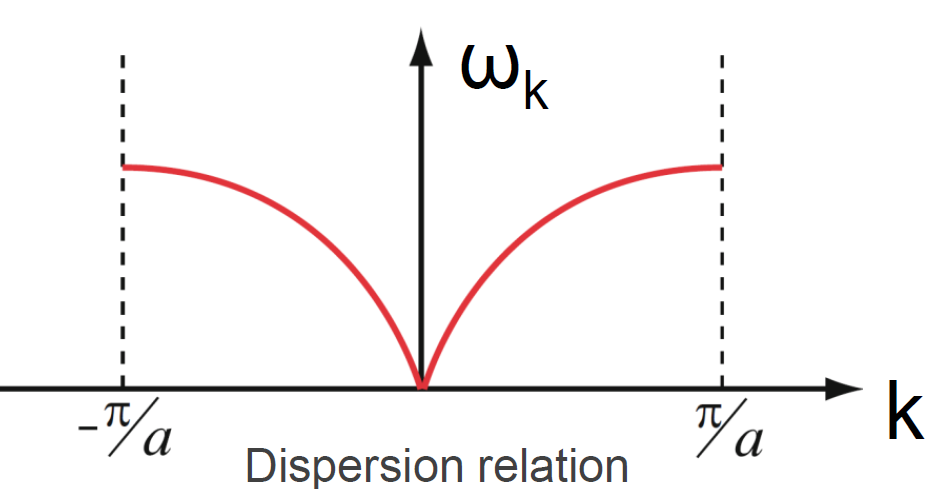
\includegraphics[width=0.6\textwidth]{figure/第一布里渊区内的色散关系.png}
                \caption{第一布里渊区内的色散关系示意图}
                \label{fig:dispertionrelationin1stBZ}
            \end{figure}
            
            那么第一布里渊区内k的取值是什么呢?我们需要考虑这个方程组的边界条件。我们可以知道,由于晶胞是有边界的,因此首尾原子不满足运动方程,但是由于边界的尺度是远远小于晶体的尺度,因此为了方便起见,我们令首尾的原子也满足这个运动方程。我们可以形象的将首尾原子相连进行编号来将这两个原子纳入运动方程的规律中(这种边界条件被称作Born-Karman边界条件,也称为周期性边界条件,见图\ref{fig:BKboundery}),可以明显发现,这样编号的结果导致了编号的周期性:
            \begin{figure}[H]
                \centering
                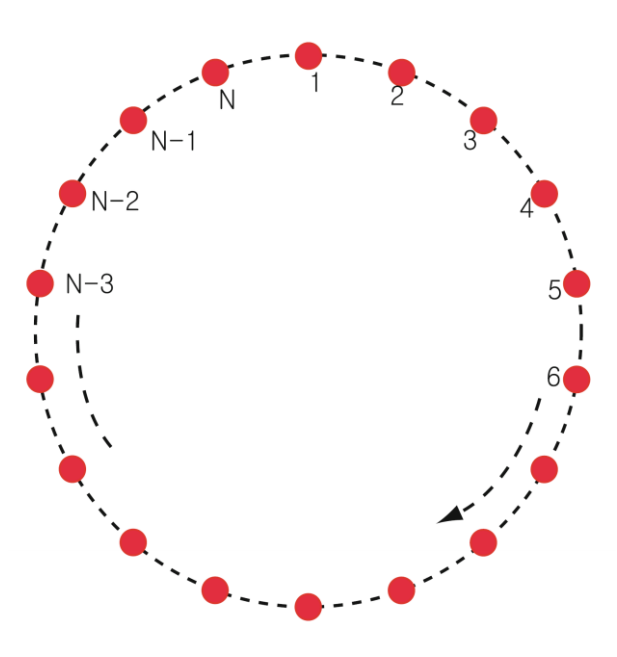
\includegraphics[width=0.6\textwidth]{figure/B-K边界条件.png}
                \caption{Born-Karman边界条件}
                \label{fig:BKboundery}
            \end{figure}
            
            即:
            \begin{equation}
                u_{n+N}=u_n
            \end{equation}
            
            代入$ u_n=A_q e^{i(kr_n-\omega t)}=A_q e^{i(k a n-\omega t)}$,我们可以知道:
            \begin{equation}
                e^{kaN}=1\Rightarrow k=\frac{2\pi m}{aN}
            \end{equation}
            
            因此当我们使用B-K边界条件导致了波矢$k$的取值是离散化的。我们可以发现,在第一布里渊区内,根据波矢的范围可以得到m的取值:
            \begin{equation}
                -\frac{\pi}{a}\leq k \leq\frac{\pi}{a}\Rightarrow -\frac{N}{2}\leq m\leq \frac{N}{2},m\in \mathbb{Z}
            \end{equation}
            
            由于对于一维单原子链来说,一个$k$对应一个$\omega$,也即对应一种格波。因此在第一布里渊区内,晶体的独立格波数目为N。
            
            最后我们考虑k在极限情况下格波的性质,我们采用相速度与群速度来描述格波传播的性质。首先明确概念:相速度的定义是相位在波中的传播速度,其定义可以表示为:
            \begin{equation}
                v_p=\frac{\lambda}{T}=\frac{\omega}{k}
            \end{equation}
            
            群速度的定义是波包中任意一个相位点的推进速度,它的定义为:
            \begin{equation}
                v_g=\frac{d\omega}{dk}
            \end{equation}
            
            在一维单原子链模型中,相速度和群速度的关系是可求的:
            \begin{align}
                \begin{split}
                    v_p=&\frac{\omega}{k}=2\sqrt{\frac{\beta}{m}}\frac{|\sin{\frac{ak}{2}}|}{k}\\
                    v_g=&\frac{d\omega}{dk}=\pm a\sqrt{\frac{\beta}{m}}\cos{\frac{ak}{2}}
                \end{split}
            \end{align}
            
            当波矢接近于0,也就是所谓的长波极限时。此时波矢点位于布里渊区中心,此时群速度和相速度可以化简为:
            \begin{align}
                \begin{split}
                    v_p=&2\sqrt{\frac{\beta}{m}}\frac{|\sin{\frac{ak}{2}}|}{k}\xrightarrow[k\rightarrow 0]{\sin{\frac{ak}{2}}\sim \frac{ak}{2}} a\sqrt{\frac{\beta}{m}}\\
                    v_g=& \pm a\sqrt{\frac{\beta}{m}}\cos{\frac{ak}{2}} = \pm a\sqrt{\frac{\beta}{m}}=|v_p|
                \end{split}
            \end{align}
            
            这种振动的模式可以类比于弹性波在连续介质内的传播,并且对于声波来说,声速=波长$\times$频率,即$\omega$和$k$成正比。当$k\rightarrow 0$时,晶格的色散关系于声波相似,因此我们称这种色散关系为声频支格波(acoustic branch)
            
            当$k=\frac{\pi}{a}$时,也就是所谓的短波极限时。此时波矢点位于布里渊区的边界上,此时群速度和相速度为:
            \begin{align}
                \begin{split}
                    v_p=&2\sqrt{\frac{2\beta}{m}}\\
                    v_g=& 0
                \end{split}
            \end{align}
            
            由于群速度为0,因此我们知道此时的振动模式为驻波。我们对一维单原子链的晶格振动结论进行简单总结:
            \begin{itemize}
                \item 一个波矢$k$对应一个$\omega$(或者说对应一种格波);
                \item 由于色散关系关于倒空间平移矢量具有平移不变性,因此我们只需要考虑第一布里渊区的独立格波即可;
                \item 由于B-K边界条件,导致第一布里渊区内k只能取离散值。第一布里渊区可取的波矢数目等于晶体的原胞数;
                \item 晶体的独立振动模式(独立格波数)=晶体的自由度数
            \end{itemize}
            
            这些结论在一维双原子链模型中也有相对应的关系,我们根据一维的两个模型就可以推广到三维的晶格振动。
            \subsubsection{一维双原子链}
                本节我们讨论一个稍微复杂的模型——一维双分子链,我们的思考逻辑与一维单原子链相同,按照“运动方程$\rightarrow$色散关系$\rightarrow$格波”的主线进行讨论。对于一维双原子链(如图\ref{fig:1Ddiatomic}),我们假设晶格常数为a,每个原子之间间距$\frac{a}{2}$;晶胞数为N,则晶体内原子总数为2N。设原胞内的原子质量分别为$M$,$m$,并且不妨假设$M>m$,同时假设第n个原胞内的相对位移分别为$u_n,v_n$。
                \begin{figure}[H]
                    \centering
                    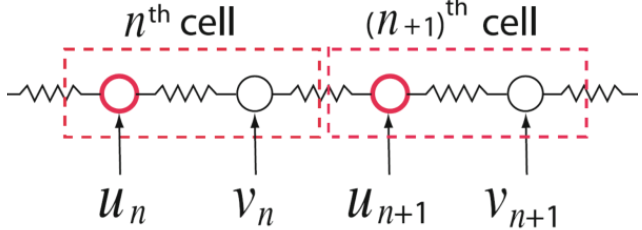
\includegraphics[width=0.6\textwidth]{figure/一维双原子链模型.png}
                    \caption{一维双原子链示意图}
                    \label{fig:1Ddiatomic}
                \end{figure}
                
                由于每个原子之间的间距相等,因此对应的$\beta$都是相等的。由此我们可以写出对应的运动方程:
                \begin{align}
                    \begin{split}
                        M\ddot{u_n}=&\beta(v_n+v_{n-1}-2u_n)\\
                        m\ddot{v_n}=&\beta(u_n+u_{n+1}-2v_n)
                    \end{split}
                \end{align}
                
                对于该运动方程,我们同样给出平面波试探解\footnote{注意,由于e指数中的第一项表示相位,两种原子的相位不同}:
                \begin{align}
                    \begin{split}
                        u_n=&A e^{i(nak-\omega t)}\\
                        v_n=&B e^{i[(n+\frac{1}{2})ak-\omega t]}
                    \end{split}
                \end{align}
                
                代入运动方程可得:
                \begin{align}
                    \begin{split}
                        (2\beta-M\omega^2)A-2\beta\cos{\frac{ak}{2}}B=&0\\
                        -2\beta\cos{\frac{ak}{2}}A+(2\beta-m\omega^2)B=&0
                    \end{split}
                \end{align}
                
                如果我们将A,B看作变量,那么这个二元一次方程组有解的充要条件是系数行列式为0,即:
                \begin{equation}
                    \begin{vmatrix}
                        2\beta-M\omega^2 & -2\beta\cos{\frac{ak}{2}}\\
                        -2\beta\cos{\frac{ak}{2}}& 2\beta-m\omega^2
                    \end{vmatrix}=0
                \end{equation}
                
                这是一个关于$\omega^2$的一元二次方程,我们可以得到对应的色散关系:
                \begin{align}\label{equ3}
                    \begin{split}
                        \omega_+=&\frac{\beta}{Mm}[(M+m)+\sqrt{M^2+m^2+2Mm\cos{ak}}]\\
                        \omega_-=&\frac{\beta}{Mm}[(M+m)-\sqrt{M^2+m^2+2Mm\cos{ak}}]
                    \end{split}
                \end{align}
                
                与一维单原子链不同的地方在于,一维双原子链的一个波矢k值对应两个$\omega$,即对应两种格波,我们称频率较高的格波($\omega_+$)为光学支格波(optical branch),频率较低的格波($\omega_-$)为声学支格波(acoustic branch),对应的色散关系图像如图\ref{fig:dispertionrelation_1Ddiaatomic}
                \begin{figure}[H]
                    \centering
                    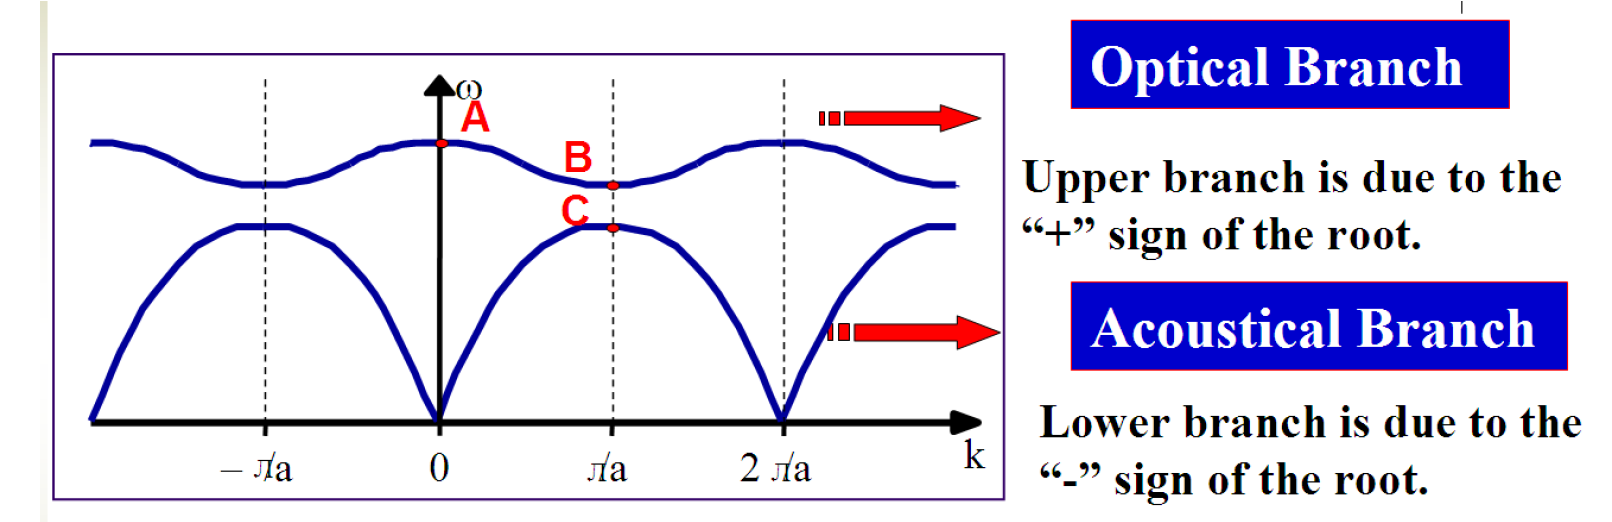
\includegraphics[width=0.6\textwidth]{figure/一维双原子链的色散关系.png}
                    \caption{一维双原子链的色散关系}
                    \label{fig:dispertionrelation_1Ddiaatomic}
                \end{figure}
                
                $\omega_-$被叫做声学支格波的原因与一维单原子链的结论相同:当$k\rightarrow 0$时,色散关系是一个线性关系:$\omega=v_sk$(当然我们也可以从群速度和相速度的角度理解);那为什么$\omega_+$被称为光学支格波呢?原因是光学声子(概念在后面会详细阐释,这里可以简单理解为代表格波的一种虚拟粒子)与光子之间能够相互作用,而理想情况下,声学声子不能与光子之间发生相互作用。因为光子的色散关系为:
                \begin{equation}
                    \omega=\frac{2\pi}{T}=\frac{2\pi c}{\lambda}=ck
                \end{equation}
                
                也就是说在光子的色散关系反应到图上是个斜率为光速c的,非常接近于纵轴的直线(如图\ref{fig:interact})。
                \begin{figure}[H]
                    \centering
                    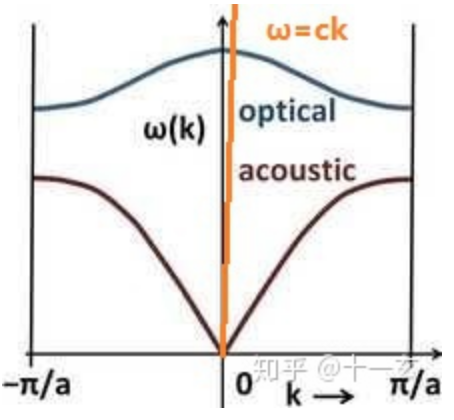
\includegraphics[width=0.6\textwidth]{figure/光子与声子的相互作用.png}
                    \caption{光子与声子的相互作用}
                    \label{fig:interact}
                \end{figure}
                
                一般来说,色散关系也可以表示为能量-动量关系,因为:
                \begin{align}
                    \begin{split}
                        E=&\hbar\omega\\
                        p=&\hbar k
                    \end{split}
                \end{align}
                
                因此,图\ref{fig:interact}中的交点代表能量守恒和动量守恒的点,也就是这个物理过程能够发生的点。对于光学声子,可以看出其色散关系与光子的色散关系在接近k=0的位置上,而其能量有值,也就是说二者可以进行能量交换,换句话说就是光子的能量可以被光学声子吸收。就是光学支格波名称的由来。
                
                我们下面分三个部分说明一维双原子链格波的性质:长波极限与短波极限下格波频率$\omega$的取值,原胞内相邻两原子的位移比,波矢k的取值。
                
                \begin{itemize}
                    \item 首先分析长波极限与短波极限下,我们可以得到$k$位于布里渊区中心和布里渊区边界情况下$\omega$的取值,具体如下表:
                \begin{center}
                    \begin{tabular}{c|c c}
                    \hline
                    \quad & $\omega_+$ & $\omega_-$\\
                    k=0 & $\sqrt{2\beta(\frac{1}{M}+\frac{1}{m})}$ & 0\\
                    $k=\frac{\pi}{a}$ & $\sqrt{\frac{2\beta}{m}}$ & $\sqrt{\frac{2\beta}{M}}$\\
                    \hline
                \end{tabular}
                \end{center}
                
                可以看到,光学支与声学支在布里渊区边缘有带隙,也就是所谓的禁带,在$\sqrt{\frac{2\beta}{M}}$到$\sqrt{\frac{2\beta}{m}}$之间,没有振动存在。
                \item 现在我们分析原胞内相邻两原子的位移比,由试探解的定义,我们知道为位移比可以表示为格波的振幅之比$\frac{A}{B}$。根据\eqref{equ3}式,我们知道:
                \begin{equation}\label{equ4}
                    \frac{A}{B}=\frac{2\beta\cos{ak}}{2\beta-M\omega^2}=\frac{2\beta-m\omega^2}{2\beta\cos{ak}}
                \end{equation}
                
                首先考虑声学支格波,由于此时$\omega\in\Big[0,\sqrt{\frac{2\beta}{M}}\Big]$,所以$2\beta-M\omega^2>0$,即$\frac{A}{B}>0$,因此声学支格波中两个原子的运动是同向的。当长波极限时。$k\rightarrow 0,\omega\rightarrow 0$,此时$\frac{A}{B}=1$,这表示两个原子会做等幅同向的运动,我们可以将其理解为原胞整体的平动或原胞质心的运动;当短波极限时,即$k\rightarrow\pm\frac{2\pi}{a},\omega\rightarrow \sqrt{\frac{2\beta}{M}}$,此时$\frac{A}{B}=\infty$,我们可以理解为轻原子不动,重原子振动。
                
                其次我们考虑光学支格波,由于此时$\omega\in\Big[\sqrt{\frac{2\beta}{m}},\sqrt{2\beta(\frac{1}{m}+\frac{1}{M})}\Big]$,所以$2\beta-m\omega^2<0$,即$\frac{A}{B}<0$,因此光学支格波中两个原子的运动是反向的。当长波极限时,即$k\rightarrow 0,\omega\in\sqrt{2\beta(\frac{1}{m}+\frac{1}{M})}$,则$\frac{A}{B}=-\frac{m}{M}$,这表明长波极限下,光学支格波的运动符合动量守恒,因此两个原子的运动虽然反向,但是质心不移动,我们可以将其理解为原胞内原子间的相对运动;当短波极限时,即$k\rightarrow\pm\frac{2\pi}{a},\omega\rightarrow \sqrt{\frac{2\beta}{m}}$,此时$\frac{A}{B}=0$,我们可以理解为重原子不动,轻原子振动。
                \item 最后我们考虑波矢k的取值,与一维单原子链相似,我们同样可以定义独立格波,从而将k的取值限制在第一布里渊区$k\in[-\frac{2\pi}{a},\frac{2\pi}{a}]$内;同样的,一维双原子链也满足B-K边界条件,即$k=\frac{2\pi}{Na}m,m\in\mathbb{Z}$。我们同样可以得到$-\frac{N}{2}\leq m\leq \frac{N}{2}$,即有N个取值,等于晶体的原胞数。但是与一维单原子链不同的是,在这里一个k对应一个声学支,一个光学支的两个$\omega$,因此总的独立格波数目为2N,等于晶体的自由度数(原胞数N$\times$每个原胞内的原子数2)。这与我们在一维单原子链中总结的结论类似。
                \end{itemize}
            
            \subsubsection{格波的量子化}
            晶体的许多热学性质与热学量(如热容)都与晶格振动的能量有关,因此本节我们讨论晶格振动的能量,我们在这里使用的方法是经典力学中处理小振动问题采用的方法。
            
            我们首先想到最直观的想法是:晶格振动的能量是所有格波能量之和吗?即:
            \begin{equation}
                E=\sum_k \hbar\omega_k
            \end{equation}
        
            由于能量也可以表示为动能与势能之和,即:
            \begin{align}
                \begin{split}
                    E=T+V=\frac{m}{2}\sum_{n=1}^{N}(\dot{u_n})^2+e^{inak}+\frac{\beta}{2}\sum_{n}(u_n-u_{n+1})^2
                \end{split}
            \end{align}
    
            我们可以最直观的发现能量的表示与第n个原子的位移$u_n$有关。在之前内容中我们已经知道晶格的振动(格波)代表了原子的一种集体振动。如果对于有N个原子一维单原子链来说,那么我们需要用N个相互关联的原子描述一支格波,用N$\times$N个参数来描述总的晶格振动。
            
            举一个简单的例子,在之前我们已经知道一维单原子链的位移解:
            \begin{equation}
                u_n=A(k)e^{i(nak-\omega t)}
            \end{equation}
            
            但是这个解只是原子振动在某个边界条件下的特解,如果要描述一般的振动模式,其形式应该是特解的线性叠加:
            \begin{equation}\label{equ:5}
                u_n=\sum_k A(k)e^{i(nak-\omega t)}
            \end{equation}
    
            那么我们自然就会思考一个问题:能否用一种更简单的方式描述晶格振动呢?观察\eqref{equ:5},我们可以将e指数中含有时间的部分是可以并入振幅项,即:
            \begin{equation}
                u_n=\sum_k B_k(t)e^{inak}
            \end{equation}
            
            由于$e^{inak}$代表相位,对于了解格波能量并无帮助,因此我们思考格波,并不需要知道每个原子在t时刻的位置,而只要确定不同波矢k下格波对应的振幅$B_k(t)$,那么我们也就知道了振动情况。换句话说,格波与格波之间其实是独立的,同时、因此我们的目标是建立一个由原子的集体振动构成的坐标系,使得格波与格波之间发生“解耦”。
            
            那么原子间发生耦合表现在能量中的哪一项呢?可以发现势能项中存在交叉项$u_nu_{n+1}$,这就是原子间相互关联的“罪魁祸首”,在线性代数中,我们可以利用二次型来描述势能函数:
            \begin{equation}
                V=\frac{\beta}{2}\sum_{n}(u_n-u_{n+1})^2=u^TBu
            \end{equation}
    
            其中:
            \begin{align}
                \begin{split}
                    u=&\begin{pmatrix}
                         u_1\\
                         u_2\\
                         \vdots\\
                         u_n\\
                         \vdots
                    \end{pmatrix}\\
                    B=&\begin{pmatrix}
                        \beta & -\frac{\beta}{2} & 0 & \cdots & 0\\
                        -\frac{\beta}{2} & \beta & -\frac{\beta}{2} & \cdots & 0\\
                        0 & -\frac{\beta}{2} & \beta & \cdots & 0\\
                        \vdots & \vdots & \vdots & \ddots & \vdots\\
                        0 & \cdots & \cdots & -\frac{\beta}{2} & \beta 
                    \end{pmatrix}
                \end{split}
            \end{align}
            
            如此,我们的问题就转化为了:通过对坐标矩阵u进行正交变换,使得系数矩阵B对角化:
            \begin{equation}
                u=AQ\Rightarrow V=u^TBu=Q^TA^TBAQ=Q^T\Lambda_BQ
            \end{equation}
            
            其中:
            \begin{align}
                \begin{split}
                    u=&\begin{pmatrix}
                         Q_1\\
                         Q_2\\
                         \vdots\\
                         Q_n\\
                         \vdots
                    \end{pmatrix}\\
                    \Lambda_B=&\frac{1}{2}\begin{pmatrix}
                        \omega^2_1 & 0 & 0 & \cdots & 0\\
                        0 & \omega^2_2 & 0 & \cdots & 0\\
                        0 & 0 & \omega^2_3 & \cdots & 0\\
                        \vdots & \vdots & \vdots & \ddots & \vdots\\
                        0 & \cdots & \cdots & 0 & \omega_N^2 
                    \end{pmatrix}
                \end{split}
            \end{align}
            
            观察$u=AQ$,矩阵u中的元素是在笛卡尔坐标系下的坐标,矩阵Q中的元素是在新的坐标系下的坐标,我们称为简正坐标(normal coordinate),A矩阵是变换矩阵,矩阵元代表新坐标系的基。根据二次型理论,我们可以得到简正坐标和基对应的形式:
            \begin{align}
                \begin{split}
                    a_{ns}=&\sqrt{\frac{1}{mN}}e^{inak_s}\\
                    Q_s=&\sqrt{mN} A(q_s) e^{-\omega(q_s)t}
                \end{split}
            \end{align}

            代入能量公式中,我们可以得到:
            \begin{equation}
                E=T+V=\frac{m}{2}\sum_{Q_s}\dot{Q_s}^2+\frac{\beta}{2}\sum_{Q_s}\omega^2|Q_s|^2
            \end{equation}
            
            可以发现,上式等价于一个谐振子的能量。一维单原子链的晶格振动可以等价为N个独立谐振子的能量之和。根据量子力学的知识,我们可以知道,一维谐振子的能量为:
            \begin{equation}
                E_k=(n_k+\frac{1}{2})\hbar\omega_k
            \end{equation}
            
            其中$\omega_k$是晶格振动频率。那么晶格振动的总能量可以表示为:
            \begin{equation}
                E=\sum_k (n_k+\frac{1}{2})\hbar\omega_k
            \end{equation}
            
            可以看到,晶格振动的能量也是量子化的,因此我们人为定义晶格振动的能量被一种准粒子(quasiparticle)——声子(phonon)所携带,那么自然$\hbar\omega_k$为声子能量。
            
            这里做几点说明:
            \begin{itemize}
                \item 一维单原子链的结论可以很容易推广到三维,下一章会进行系统的总结。
                \item 为什么声子叫做准粒子?因为声子可以定义所谓的准动量$\hbar k$,但是声子并不是真实存在的粒子,因为无法脱离晶格而存在。我们定义声子的好处在于,当我们考虑电子或者光子与晶格振动相互作用时,我们就可以等效为其与能量为$\hbar\omega_k$,动量为$\hbar k$的粒子相互作用,物理图像就变得非常清晰了。
                \item 声子是晶格振动的能量量子,也是晶体原子集体运动状态的激发单元(所谓的一种元激发的概念)。
                \item 一种格波(或一种振动模式)被称为一种声子,当这种声子处于$(n_k+\frac{1}{2})\hbar \omega_k$本征态的时候,这种声子的声子数为$n_k$,简单的示意图可以如图\ref{fig:phonon}:
                \begin{figure}[H]
                    \centering
                    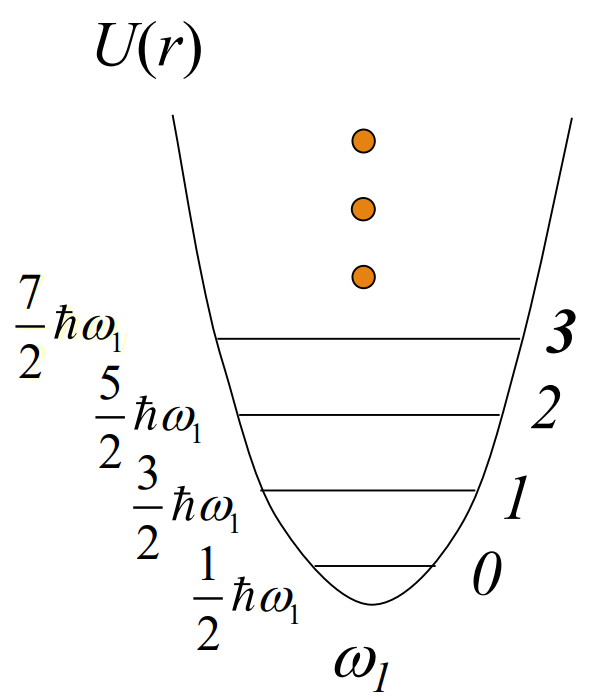
\includegraphics[width=0.5\textwidth]{figure/声子.png}
                    \caption{声子能级示意图}
                    \label{fig:phonon}
                \end{figure}
                \item 由于晶体中可以激发任意多数目的声子,因此声子服从玻色-爱因斯坦分布,其平均声子数可以表示为:
                \begin{equation}
                    \Bar{n_k}=\frac{1}{e^{-\frac{\hbar\omega_k}{k_BT}}-1}
                \end{equation}
            \end{itemize}
            
            \subsection{三维晶体的振动模式}
            
            根据上面两节的讨论,我们已经获得了一维晶格振动的图像,本节,我们希望从动力学方程与能量两个主要方面将一维的模型拓展到三维。
            
            \subsubsection{动力学方程、色散关系与格波的性质}
            首先我们讨论三维晶格振动的动力学方程与色散关系。我们假设三维晶体有N个原胞,每个原胞内有r个原子。其中第l个原胞的第s个原子的质量为$m_s$,平衡位置为$\vec{R}\binom{l}{s}$,偏离平衡位置的位移为$\vec{u}\binom{l}{s}$,位移在$\alpha$方向上的分量为$\vec{u_\alpha}\binom{l}{s}$。那么该原子沿$\alpha$方向的运动方程可以写作:
            \begin{equation}\label{equ:motion2}
                m_s\ddot{u_\alpha}\binom{l}{s}=-\sum_{\beta,l',s'}\phi_{\alpha,\beta}\begin{pmatrix}
                l & l'\\
                s & s'
                \end{pmatrix}[u_\alpha\binom{l}{s}-u_\beta\binom{l'}{s'}]
            \end{equation}
            
            其中$\phi_{\alpha,\beta}\begin{pmatrix}
                l & l'\\
                s & s'
                \end{pmatrix}$是第l个原胞第s个原子和第l'个原胞第s'个原子之间的准弹性相互作用力常数,这个常数只和原子间的相对距离有关,于是力常数可以表示为:
                \begin{equation}
                    \phi_{\alpha,\beta}\begin{pmatrix}
                l & l'\\
                s & s'
                \end{pmatrix}=\left[\frac{\partial^2 V}{\partial u_\alpha\binom{l}{s}\partial u_\beta\binom{l'}{s'}}\right]_0=\phi_{\alpha,\beta}\binom{l-l'}{s\quad s'}
                \end{equation}
                
                试探解的形式与一维情况类似:
                \begin{equation}
                    u\binom{l}{s}=A(\vec{k})e^i[\vec{R_l}\cdot \vec{k}-\omega(\vec{k})t]
                \end{equation}
                
                其中$A(\vec{k})$是振幅,其分量为$A_\alpha,A_\beta,A_\gamma$,代入运动学方程\eqref{equ:motion2}式,可得:
                \begin{equation}
                    \sum_{\beta,s'}\Big(m_s\omega(\vec{k})^2\delta_{\alpha\beta}\delta_{ss'}-\sum_l'\phi_{\alpha,\beta}\binom{l-l'}{s\quad s'}e^{i(\vec{R_l}-\vec{R_{l'}})\cdot \vec{k}}\Big)A_\beta=0
                \end{equation}
                
                我们令$D_{\alpha\beta}^{ss'}(\vec{k})=\sum_l'\phi_{\alpha,\beta}\binom{l-l'}{s\quad s'}$,称为动力学矩阵,那么上式是一个3r阶齐次方程组,它含有非零解的充要条件是:
                \begin{equation}
                    \det{\Big(m_s\omega(\vec{k})^2\delta_{\alpha\beta}\delta_{ss'}-D_{\alpha\beta}^{ss'}\Big)}=0
                \end{equation}
                
                这是一个$3r\times 3r$阶行列式,通过求解行列式,我们可以得到3r个$\omega\sim \vec{k}$的关系,即3r支格波。在之前的讨论中,我们知道声学波代表晶格的集体振动,光学波代表晶格原胞原子的相对运动。因此三维晶格声学波一定只有3支,那么光学波有3r-3支。
                
                下面讨论波矢数和格波频率数的关系。讨论波矢数的关系需要我们获得倒空间的相关信息。假设晶体有N个原胞,原胞基矢分别为$\vec{a_1},\vec{a_2},\vec{a_3}$,并且在基矢方向上的原胞数分别是$N_1,N_2,N_3$,于是$N=N_1N_2N_3$,三维晶胞仍然满足B-K边界条件,于是我们可以得到对应的边界条件:
                \begin{equation}\label{equ:F}
                    \vec{u}\binom{l}{s}=\vec{u}\binom{l+N_i}{s}\Rightarrow N_i\vec{a_i}\cdot\vec{k}=2\pi m_i,i=1,2,3
                \end{equation}
                
                考虑格波的波矢$\vec{k}=k_1\vec{b_1}+k_2\vec{b_2}+k_3\vec{b_3}$,结合正格子与倒格子基矢的关系:$\vec{a_i}\cdot\vec{b_j}=2\pi m\delta_{ij}$,结合\eqref{equ:F}式,我们可以得到格波波矢坐标$k_i$的关系:
                \begin{equation}
                    k_i=\frac{m_i}{N_i}
                \end{equation}
                
                那么格波波矢的形式为:
                \begin{equation}
                    \vec{k}=m_1\frac{\vec{b_1}}{N_1}+m_2\frac{\vec{b_2}}{N_2}+m_3\frac{\vec{b_3}}{N_3}
                \end{equation}
                
                由此我们可以得到一个格波波矢代表点所围成的体积为:
                \begin{equation}
                    \frac{\vec{b_1}}{N_1}\cdot(\frac{\vec{b_2}}{N_2}\times\frac{\vec{b_3}}{N_3})=\frac{(2\pi)^3}{N\Omega}=\frac{(2\pi)^3}{V}
                \end{equation}
                
                其中V是晶胞的体积。有了上述内容铺垫,我们可以求得波矢数和格波频率数的关系了。与一维晶格相同,晶格振动在倒空间中同样具有周期性:
                \begin{align}
                    \begin{split}
                        u_\alpha\binom{l}{s}(\vec{k}+\vec{K_h})=&A_\alpha e^{i[\vec{R_l}\cdot(\vec{k}-\vec{K_h})-\omega(\vec{k})t]}\\
                        =&A_\alpha e^{i[\vec{R_l}\cdot\vec{k}-\omega(\vec{k})t]}\\
                        =&u_\alpha\binom{l}{s}(\vec{k})
                    \end{split}
                \end{align}
                
                由此,我们只需要考虑第一布里渊区的振动情况即可。我们已经知道了一个格波波矢点所围成的体积是$\frac{(2\pi)^3}{V}$,那么单位体积内的波矢数目(称为波矢密度)自然是它的倒数:
                \begin{equation}
                    \frac{1}{\frac{(2\pi)^3}{V}}=\frac{V}{(2\pi)^3}
                \end{equation}

                于是,在第一布里渊区内,波矢的数目为:
                \begin{equation}
                     \Omega^*\cdot\frac{V}{(2\pi)^3}=\frac{\Omega^*N\Omega}{(2\pi)^3}=N
                \end{equation}
                
                因此我们就验证了一维晶格振动的结论:
                \begin{itemize}
                    \item 晶格振动的波矢数=原胞数
                    \item 独立格波个数=原胞内原子的自由度数(=维数$\times$原胞内原子个数)
                    \item 格波频率数 = 晶体自由度数(=原胞内原子的自由度数$\times$原胞数)
                \end{itemize}
                
                \subsubsection{利用准经典近似求解晶格振动能量}
                根据一维晶格的振动,我们可以推广得到三维晶格的总能量是所有声子的能量之和:
                \begin{equation}
                    E=\sum_\lambda^{3N}\sum_{k=1}^N\Bar{E_{\lambda k}}=\sum_\lambda^{3N}\sum_{k=1}^N(n_{\lambda k}+\frac{1}{2})\hbar\omega_{\lambda k}
                \end{equation}
                
                其中,平均声子数满足$n_{\lambda k}=\frac{1}{e^{-\frac{\hbar\omega_k}{k_BT}}-1}$。但是由于宏观晶体对应的格波数很大,接近$10^{23}$量级,因此离散求和得到能量是不现实的。为了得到晶格振动的能量,我们采用所谓准经典近似的方法\footnote{这也是统计物理常用的方法}:其原理在于宏观晶体的原胞数N很大,而在第一布里渊区内,k的取值等于N,因此我们可以近似的认为k的取值是连续的,这样我们就可以将离散求和转化为积分:
                \begin{align}
                    \begin{split}
                        E=&\sum_\lambda^{3N}\sum_{k=1}^N\Bar{E_{\lambda k}}\\
                        =&\sum_\lambda^{3N}\int_{k\in 1^{st}BZ}\Bar{E_{\lambda k}}\frac{V}{(2\pi)^3}d\vec{k}\\
                        =&\sum_\lambda^{3N}\int_{k\in 1^{st}BZ}\frac{V}{(2\pi)^3}d\vec{k}\int_0^\infty (n_{\lambda k}+\frac{1}{2})\hbar\omega\delta(\omega-\omega_k)d\omega\\
                        =&\int_0^\infty (\frac{1}{e^{-\frac{\hbar\omega}{k_BT}}-1}+\frac{1}{2})\hbar\omega d\omega\sum_\lambda^{3N}\int_{k\in 1^{st}BZ}\frac{V}{(2\pi)^3}\delta(\omega-\omega_k)d\vec{k}
                    \end{split}
                \end{align}
                
                其中 上式的第二个等号需要乘以波矢密度$\frac{V}{(2\pi)^3}$,原因在于离散求和的时候是对所有的波矢$\vec{k}$求和,而在$d\vec{k}$空间内的波矢数为$\frac{V}{(2\pi)^3}d\vec{q}$;第三个等号运用了$\delta$函数的筛选性质。
                
                我们可以将E的式子拆分为两项来看,对$\omega$的积分部分表明了声子的能量之和,对$d\vec{k}$的积分则是表明振动模式数。为了简化,令:
                \begin{equation}
                    g_\lambda(\omega)=\int_{k\in 1^{st}BZ}\frac{V}{(2\pi)^3}\delta(\omega-\omega_k)d\vec{k}
                \end{equation}
                
                自然,将所有的$g_\lambda(\omega)$对简正坐标自由度求和可以得到体积为V的晶体单位频率内的振动模式数\footnote{那究竟为什么$\delta$函数可以代表模式密度呢?其原因在于它是突跃函数的导数。我们定义突跃函数\begin{equation*}
                    \theta(\omega-\omega_\lambda(\vec{k}))=\begin{cases}
                    1 & \omega_\lambda(\vec{k})<\omega\\
                    0 & \omega_\lambda(\vec{k})>\omega
                    \end{cases}
                \end{equation*}
                
                我们可以将所有$\vec{k}$对应的$\theta$函数相加,就可以得到(0,$\omega$)内的模式数:
                \begin{equation*}
                    Z(\omega)=\sum_{\vec{k}}\theta(\omega-\omega_\lambda(\vec{k}))
                \end{equation*}
                
                因此模式数对$\omega$的导数,即单位频率内的模式数的形式可以用$\delta$函数表示:
                \begin{equation*}
                    \frac{dZ}{d\omega}=\sum_{\vec{k}}\delta(\omega-\omega_\lambda(\vec{k}))
                \end{equation*}},我们称之为模式密度,记作$g(\omega)$:\begin{equation}
                    g(\omega)=\sum_\lambda^{3N}g_\lambda(\omega)
                \end{equation}
                
                $g(\omega)$表明体积为V的晶体单位频率内的模式数,那么对于单位体积的晶体,单位频率内的模式数我们用$D(\omega)$表示,我们称之为声子态密度或频谱密度。根据定义求$D(\omega)$是十分困难的,因此我们采用另一种模式求$D(\omega)$。我们考虑单位体积内$\omega\sim\omega+d\omega$间的振动模式数$dN$,如果能求解出$dN$,根据定义:
                \begin{equation}
                    D(\omega)=\frac{dN}{d\omega}
                \end{equation}
                
                求解的核心在于振动模式数等于波矢数,因此$dN$可以表示为单位体积内$\omega\sim\omega+d\omega$间的波矢数,一种振动模式对应的波矢数等于波矢空间内$\omega\sim\omega+d\omega$的等频率面间的体积乘以单位体积的波矢密度:
                \begin{equation}
                    dN_\lambda=\frac{1}{(2\pi)^3}\int_{S_\omega}^{S_{\omega+d\omega}} dV^*
                \end{equation}
                
                其中$dV^*$是等频率面的体积元,它可以表示为等频率面间的垂直距离$dl^*$和面积元$dS^*$的乘积:
                \begin{equation}
                    dV^*=dl^*\times dS^*
                \end{equation}
                
                而根据梯度的定义,梯度与$dl^*$间有关系:
                \begin{equation}
                    d\omega=|\nabla_k\omega|dl^*
                \end{equation}
                
                代入$dN_\lambda$可得:
                \begin{equation}
                     dN_\lambda=\frac{1}{(2\pi)^3}\int_{S_\omega}^{S_{\omega+d\omega}}\frac{d\omega}{|\nabla_k\omega|}dS^*
                \end{equation}
                
                由于$dN_\lambda$代表得是某一支格波对应得振动模式数,那么总的晶格振动模式数$dN$应该是所有$dN_\lambda$之和,那么晶格总得振动模式密度$D(\omega)$为:
                \begin{equation}\label{equ:D_omega}
                    D(\omega)=\sum_{j=1}^{3r}\frac{1}{(2\pi)^3}\int_{S_\omega}^{S_{\omega+d\omega}}\frac{dS^*}{|\nabla_j\omega|}
                \end{equation}
                
                特别的,如果$|\nabla_j\omega|=0$,我们称该点为范霍夫奇异点。于是我们就可以得到单位体积晶体的晶格振动能量的表达式:
                \begin{equation}\label{equ:G}
                    E=\int_0^\infty (\frac{1}{e^{-\frac{\hbar\omega}{k_BT}}-1}+\frac{1}{2})\hbar\omega D(\omega)d\omega
                \end{equation}

                
                \subsection{晶格比热容}
                从本节开始,我们将会将我们之前模型得到的结论应用于分析晶体的热学性质中。而热运动在宏观性质上最直接的表示就是热容$C_v=\frac{\partial E}{\partial T}$。上世纪,科学家将经典统计理论应用到了晶格热容,得到了所谓Dulong-Petit定律。
                
                具体来说,根据经典统计理论中的能量均分定律,每一个平动和转动自由度的平均热能为$\frac{1}{2}k_BT$,而每一个振动自由度的平均热能为$k_BT$(因为对于势能与动能各为$\frac{1}{2}k_BT$),对于晶格振动来说,没有平动和转动的自由度,因此其热能等于$3RT$,比热容为$3R$。也就是说Dulong-Petit定律认为晶体的比热容永远是一个恒定的值,不随温度和晶体种类而改变。但是这个结论仅仅在室温和高温成立,当温度处于低温时,热容会迅速降低,直至0(如图\ref{fig:heatcapacity})
                \begin{figure}[H]
                    \centering
                    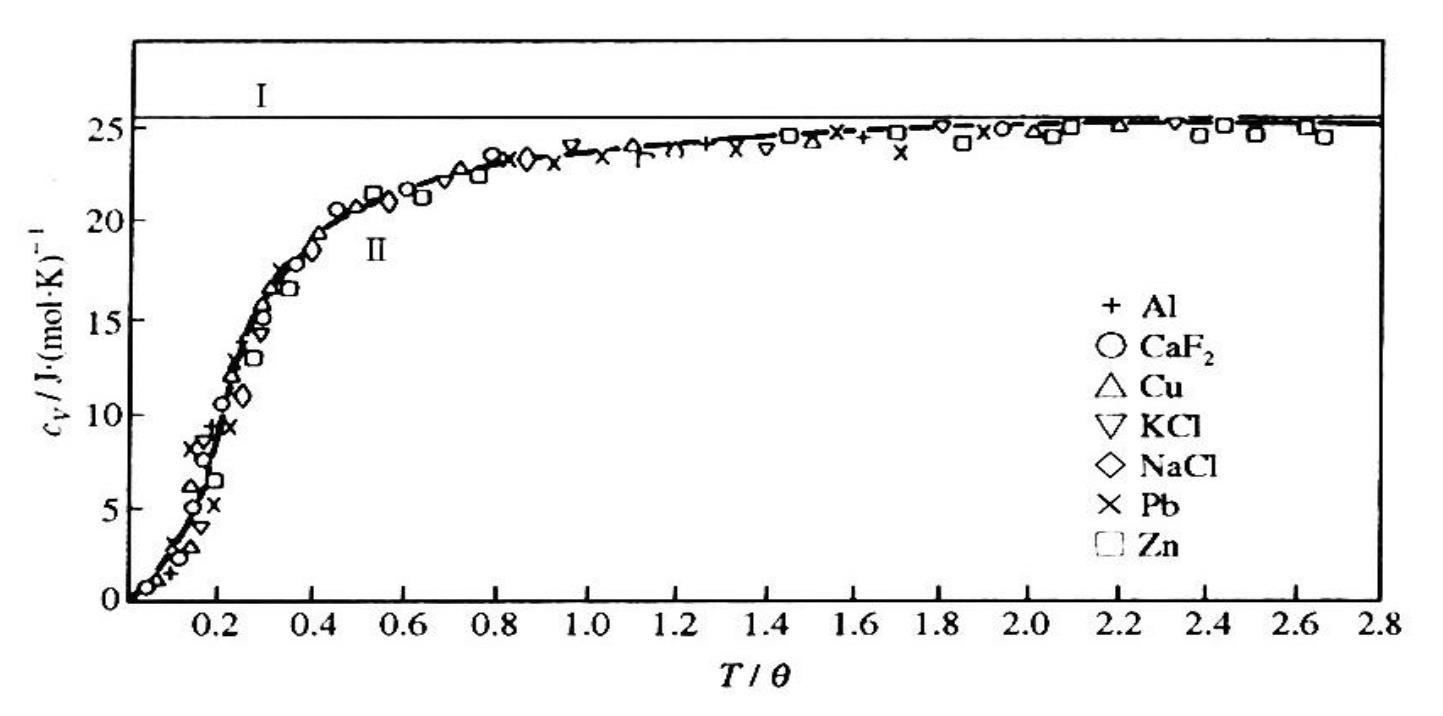
\includegraphics[width=0.7\textwidth]{figure/heatcapacity.jpg}
                    \caption{各种晶体的比热容随温度的变化曲线}
                    \label{fig:heatcapacity}
                \end{figure}
                
                根据前面的讨论,我们知道Dulong-Petit定律在低温区域失效的核心原因在于格波能量的量子化,在上节的最后我们已经得到了从格波量子化出发推导出的晶格振动能量(式\eqref{equ:G}),于是我们可以得到晶格比热容的一般表达式:
                \begin{align}\label{heatcapacity}
                    \begin{split}
                        C_v=&\left(\frac{\partial E}{\partial T}\right)_V\\
                        =&\int_0^\infty \frac{e^{-\frac{\hbar\omega}{k_BT}}\frac{\hbar\omega}{k_BT^2}}{(e^{-\frac{\hbar\omega}{k_BT}}-1)^2}+\hbar\omega D(\omega)d\omega\\
                        =& \int_0^\infty \frac{e^{-\frac{\hbar\omega}{k_BT}}\frac{\hbar\omega}{k_BT^2}}{(e^{-\frac{\hbar\omega}{k_BT}}-1)^2}\Big(\frac{\hbar\omega}{k_BT}\Big)^2 k_B D(\omega)d\omega
                    \end{split}
                \end{align}
                
                可以看到,问题的关键在于建立合适的近似模型(因为格波的形式比较复杂)得到模式密度$D(\omega)$的表达式。爱因斯坦采用了最简单的假设:他假设所有晶格振动的模式都是简并的,也即:$\omega=\omega_E$,于是对应的$D(\omega)$可以写作:
                \begin{equation}
                    D(\omega)=3N\delta(\omega-\omega_E)
                \end{equation}
                
                其中N是晶胞内的原子数,3N即表明晶胞内原子的自由度数。代入\eqref{heatcapacity}式,可得:
                \begin{align}\label{equ:heatcapacity_E}
                    \begin{split}
                        C_v=&\left(\frac{\partial E}{\partial T}\right)_V\\
                        =&\frac{e^{-\frac{\hbar\omega_E}{k_BT}}\frac{\hbar\omega_E}{k_BT^2}}{(e^{-\frac{\hbar\omega_E}{k_BT}}-1)^2}\Big(\frac{\hbar\omega_E}{k_BT}\Big)^2 k_B 3N\omega_E\\
                        =&3Nk_B\Big(\frac{\Theta_E}{T}\Big)^2\frac{e^{\frac{\Theta_E}{T}}}{(e^{\frac{\Theta_E}{T}}-1)^2}
                    \end{split}
                \end{align}
                
                其中为了简化上式的形式,我们定义了一个含有温度量纲的物理量,即爱因斯坦温度:
                    \begin{equation}
                        \Theta_E=\frac{\hbar\omega_E}{k_B}
                    \end{equation}
                
                这个模型虽然比较粗糙,但是已经能比较好的描述比热容随温度变化的趋势了:当温度处于高温极限时,此时$T>>\Theta_E$,即$\frac{\Theta_E}{T}\rightarrow 0$ ,$(e^{\frac{\Theta_E}{T}}\approx 1+\frac{\Theta_E}{T}$,因此\eqref{equ:heatcapacity_E}可以化简为:
                \begin{equation}
                    C_v=3Nk_B\Big(\frac{\Theta_E}{T}\Big)^2\frac{1}{(\frac{1+\Theta_E}{T}-1)^2}=3Nk_B=3R
                \end{equation}
                
                此时比热容的性质回归到了Duloong-Petit定律。当温度处于低温极限时,此时$T<<\Theta_E$,即$e^{\frac{\Theta_E}{T}}>>1$。因此此时式\eqref{equ:heatcapacity_E}可以化简为:
                \begin{align}
                    \begin{split}
                     C_v=&3Nk_B\Big(\frac{\Theta_E}{T}\Big)^2\frac{e^{\frac{\Theta_E}{T}}}{(e^{\frac{\Theta_E}{T}}-1)^2}\\
                     =&3Nk_B\Big(\frac{\Theta_E}{T}\Big)^2\frac{e^{\frac{\Theta_E}{T}}}{(e^{\frac{\Theta_E}{T}})^2}\\
                     =&3Nk_B\Big(\frac{\Theta_E}{T}\Big)^2e^{-\frac{\Theta_E}{T}} \\
                     =& 0
                    \end{split}
                \end{align}
                
                虽然爱因斯坦模型能够描述比热容随温度变化的大概趋势,但是根据实验与理论对照(如图\ref{fig:Einsteinmodel_A}),我们可以知道爱因斯坦模型在低温的时候与实验不符,这是为什么呢?
                \begin{figure}[H]
                    \centering
                    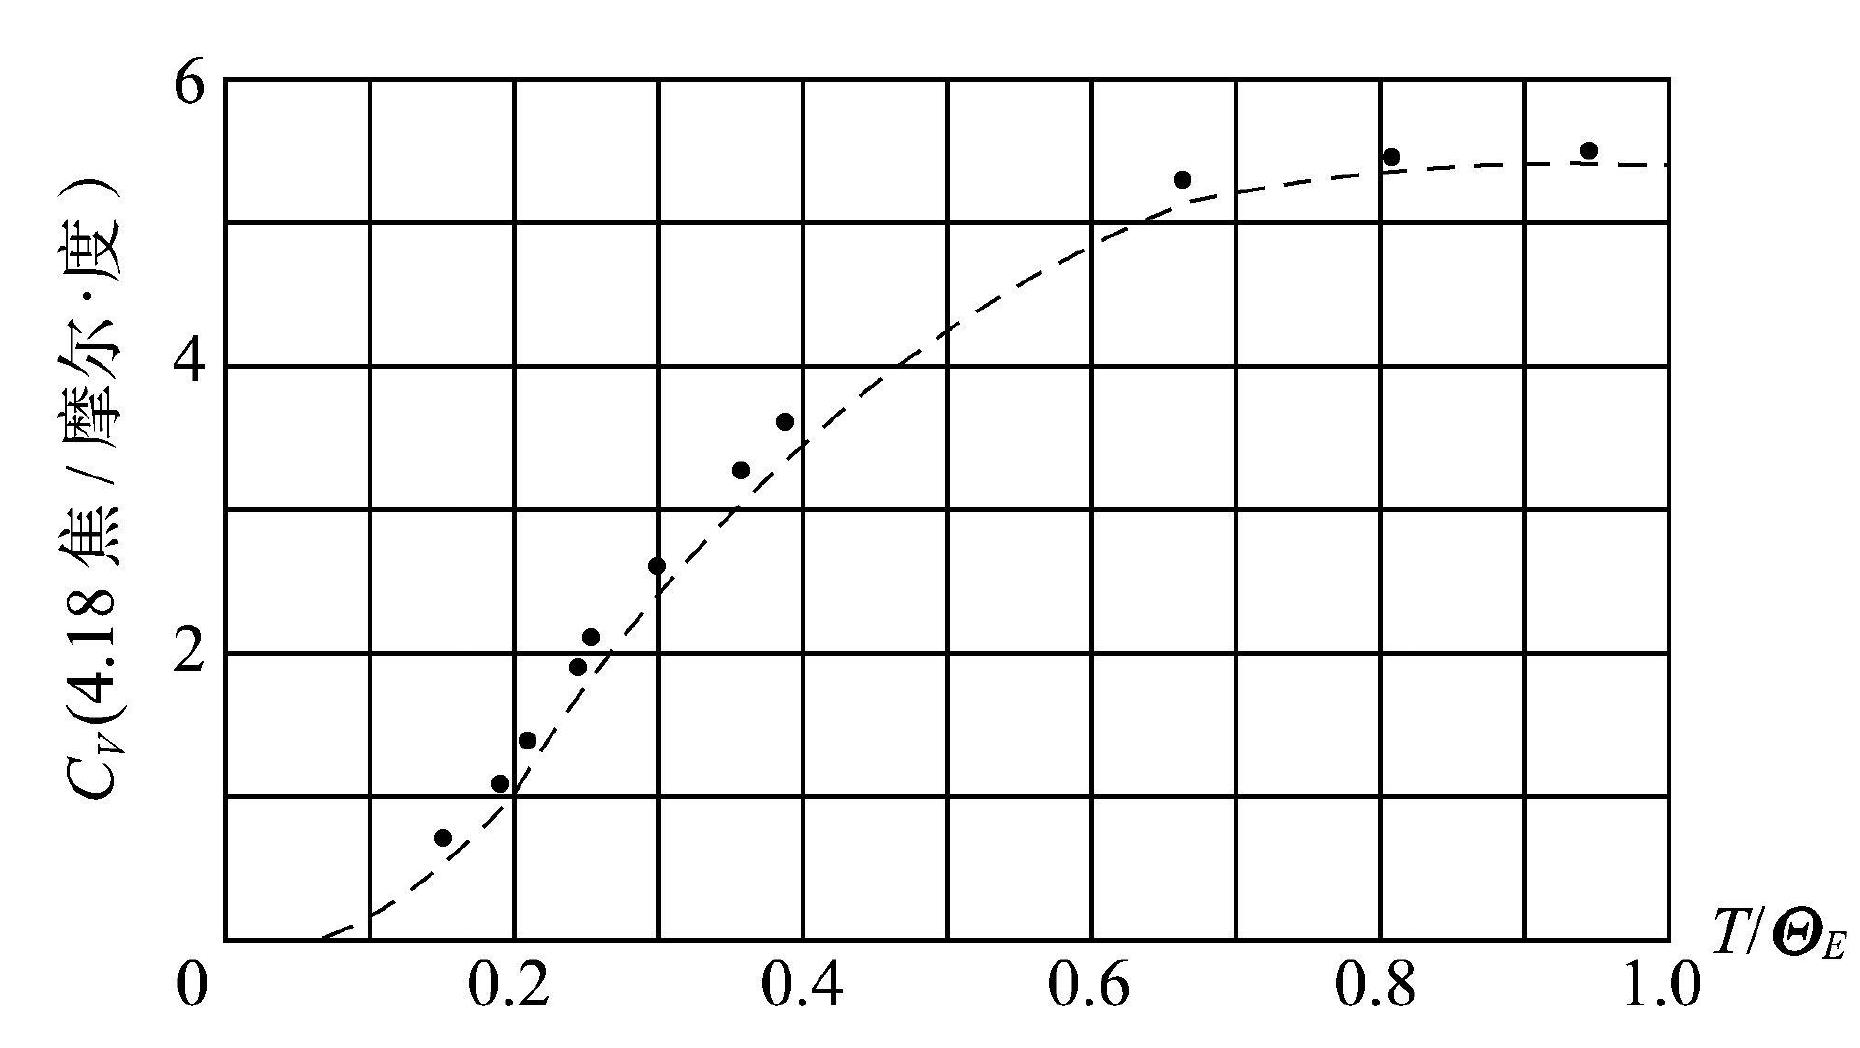
\includegraphics[width=0.6\textwidth]{figure/金刚石比热容随温度的关系.jpg}
                    \caption{金刚石的比热容随温度的变化关系(虚线为爱因斯坦模型理论值)}
                    \label{fig:Einsteinmodel_A}
                \end{figure}
                
                爱因斯坦模型设定的频率$\omega_E$约为$10^{13}Hz$,处于光学波;而具体计算可以知道,当晶格处于低温时,格波的频率应该属于声学波的范围,这是导致偏差的本质原因。Debye基于这种现象提出了Debye模型。
                
                Debye对晶格作了另外一种近似,由于晶格在低温时频率处在声学波范围内,于是他假设晶格是一种弹性连续介质,由此可以得到最核心的两个假设:
                \begin{enumerate}
                    \item 与经典弹性波类似,频率满足$\omega=v\vec{k}$,其中v是波速,$\vec{k}$是波矢。由于我们认为晶格是连续介质,因此$\omega$的取值是连续的。并且三维弹性波有一支纵波(longitudinal wave),两支横波(transverse wave)\footnote{横波就是波的传播方向和原子的运动方向垂直,对于三维波来说,垂直的方向有两个,因此是两个横波;纵波是波的传播方向与原子的运动方向同向,因此只有一个纵波},对应的波速和频率都是不同的:
                    \begin{align}
                        \begin{split}
                            \omega_L(\vec{k})=&v_L\vec{k}\\
                            \omega_T(\vec{k})=&v_T\vec{k}
                        \end{split}
                    \end{align}
                    \item 由于频率满足$\omega=v\vec{k}$,因此频率对波矢的梯度应该是一个常数(等于波速),即:
                    \begin{equation}
                        |\nabla_k\omega|=v=const.
                    \end{equation}
                    
                    这一点其实和第一条假设完全相同,强调梯度为常数的原因在于,如果我们考虑$\omega$在$k$空间上的轨迹时,根据梯度的定义,我们可以知道$\omega$的轨迹是一个球体,这一点是后续讨论的核心。
                \end{enumerate}
                
                但是直接将晶格近似成连续介质弹性波存在一个问题,即离散和连续的问题。具体来说,连续介质弹性波的$\omega$能从0取到$\infty$,它的振动模式数是无限的,但是晶体振动由于考虑了B-K边界条件,其波矢的取值应该等于原胞的个数N,这就产生了矛盾。Debye的处理方法非常简单:人为设定一个截止频率$\omega_D$,大于$\omega_D$的波是不存在的,而在小于$\omega_D$的振动仍然采用弹性波的近似。换一种表述方法,在k空间上,我们认为k的允许取值应该落在以$\vec{k_D}=\frac{\omega_D}{v}$为半径的球内,并且球的体积应该和第一布里渊区的体积相同,包含n个取值。我们可以用波矢密度$\times$体积来构建等式\footnote{由于考虑$D(\omega)$,因此这里的波矢密度是单位体积的波矢密度}:
                \begin{equation}
                    \frac{4\pi}{3}k_D^3\times \frac{1}{(2\pi)^3}=n
                \end{equation}
                
                我们可以得到k空间的最大半径的表达式为:
                \begin{equation}
                    k_D^3=6\pi^2 N
                \end{equation}
                
                在阐明了Debye模型的假设以及其在k空间的图像以后,我们就可以根据一支格波的声子态密度$D(\omega_j)$的关系式(式\eqref{equ:D_omega})可以得到:
                \begin{align}
                    \begin{split}
                     D(\omega_j)=&\frac{1}{(2\pi)^3}\int_{S_\omega}^{S_{\omega+d\omega}}\frac{dS^*}{|\nabla_j\omega|}\\
                     =&\frac{1}{(2\pi)^3}\frac{4\pi \vec{k}^2}{v}\\
                     =& \frac{1}{(2\pi)^3}\frac{4\pi\omega^2}{v^3}\\
                     =& \frac{\omega^2}{2\pi v^3}
                    \end{split}
                \end{align}
                
                其中第二个等号是因为等频率面是一个球,导致$dS^*$的积分可以直接用面积公式求出;第三个等号运用了连续弹性波假设$\omega=v\vec{k}$。同时注意上式的$\omega$是总频率,不是$\omega_j$。由于总的波有一个纵波两个横波,因此总的模式密度等于:
                \begin{equation}
                    D(\omega)=\frac{\omega^2}{2\pi v^3} \Big(\frac{1}{v_L^3}+\frac{2}{v_T^3}\Big)=\frac{\omega^2}{2\pi v_s^3}
                \end{equation}
                
                其中$v_s$是为了简化公式形式人为设的“平均”波速,它的定义是:
                \begin{equation}
                    \frac{1}{v_s^3}=\frac{1}{v_L^3}+\frac{2}{v_T^3}
                \end{equation}
                
                同时由于模式数等于晶胞原子的自由度3N(N是单位体积晶胞含有的原子数),因此模式密度的积分就满足:
                \begin{equation}
                    \int_0^{\omega_D} D(\omega)d\omega =3N
                \end{equation}
                
                这是一个简单的积分,我们可以得到波速$v_s$和截止频率$\omega_D$之间的关系:
                \begin{equation}
                    \omega_D=(6\pi^2N)^{\frac{1}{3}}v_s
                \end{equation}
                
                因此,模式密度可以将参数$v_s$替换成参数$\omega_D$:
                \begin{equation}
                    D(\omega)=\frac{9\omega^2N}{\omega_D^3}
                \end{equation}
                
                代入热容通式(式\eqref{heatcapacity}),可以得到:
                \begin{align}\label{equ:heatcapacity_D}
                    \begin{split}
                        C_v=&\int_0^\infty \frac{e^{-\frac{\hbar\omega}{k_BT}}\frac{\hbar\omega}{k_BT^2}}{(e^{-\frac{\hbar\omega}{k_BT}}-1)^2}\Big(\frac{\hbar\omega}{k_BT}\Big)^2 k_B D(\omega)d\omega\\
                        =& \int_0^{\omega_D} \frac{e^{-\frac{\hbar\omega}{k_BT}}\frac{\hbar\omega}{k_BT^2}}{(e^{-\frac{\hbar\omega}{k_BT}}-1)^2}\Big(\frac{\hbar\omega}{k_BT}\Big)^2 k_B \frac{9\omega^2N}{\omega_D^3}d\omega\\
                        =& 9Nk_B\Big(\frac{T}{\Theta_D}\Big)^3\int_0^{\frac{\Theta_D}{T}} \frac{e^{x}}{(e^{x}-1)^2}x^4dx 
                    \end{split}
                \end{align}
                
                上式最后一个等式定义了德拜温度$\Theta_D=\frac{\hbar\omega_D}{k_B}$和坐标变换$x=\frac{\hbar\omega}{k_BT}$作为简化。下面考虑高温极限与低温极限:
                
                当晶格温度处于高温时,此时$T>>\Theta_D$,即$\frac{\Theta_D}{T}\rightarrow 0$,此时\eqref{equ:heatcapacity_D}式可以化简为:
                \begin{align}
                    \begin{split}
                        C_v=&9Nk_B\Big(\frac{T}{\Theta_D}\Big)^3\int_0^{\frac{\Theta_D}{T}} \frac{e^{x}}{(e^{x}-1)^2}x^4dx \\
                        =&9Nk_B\Big(\frac{T}{\Theta_D}\Big)^3\int_0^{\frac{\Theta_D}{T}} \frac{1}{(e^{\frac{1}{2}x}-e^{-\frac{1}{2}x})^2}x^4dx\\
                        =&9Nk_B\Big(\frac{T}{\Theta_D}\Big)^3\int_0^{\frac{\Theta_D}{T}} \frac{1}{1+\frac{1}{2}x-(1-\frac{1}{2}x)}x^4dx\\
                        =&9Nk_B\Big(\frac{T}{\Theta_D}\Big)^3\int_0^{\frac{\Theta_D}{T}} x^2 dx\\
                        =&3Nk_B
                    \end{split}
                \end{align}
                
                此时比热容的性质同样回归为Deloong-Petit定律。当晶格温度处于低温,即$T<<\Theta_D$时,此时$\frac{\Theta_D}{T}\rightarrow \infty$,于是\eqref{equ:heatcapacity_D}可以化简为:
                \begin{align}
                    \begin{split}
                        C_v=&9Nk_B\Big(\frac{T}{\Theta_D}\Big)^3\int_0^{\frac{\Theta_D}{T}} \frac{e^{x}}{(e^{x}-1)^2}x^4dx \\
                        =&9Nk_B\Big(\frac{T}{\Theta_D}\Big)^3\int_0^\infty \frac{e^{x}}{(e^{x}-1)^2}x^4dx \\
                    \end{split}
                \end{align}
                
                计算的核心在于处理积分$\int_0^\infty \frac{e^{x}}{(e^{x}-1)^2}x^4dx$,我们在这里利用到了麦克劳林展开:
                \begin{equation}
                    (1+x)^n=1+nx+\frac{n(n-1)}{2!}x^2+\frac{n(n-1)(n-2)}{3!}x^3+\cdots
                \end{equation}
                
                于是,结合$\Gamma$函数和黎曼$\zeta$函数的性质,我们可以得到:
                \begin{align}
                    \begin{split}
                        \int_0^\infty \frac{e^{x}}{(e^{x}-1)^2}x^4dx=&\int_0^\infty e^{-x}(1-e^{-x})^{-2}x^4dx\\
                        =&  \int_0^\infty e^{-x}(1+2e^{-x}+3e^{-2x}+4e^{-3x}+\cdots)x^4dx\\
                        =& \int_0^\infty x^4 \Big(\sum_n n e^{-nx}\Big)\\
                        =& 4! \sum n\times \frac{1}{n^5}\\
                        =& 4! \zeta(4)\\
                        =& \frac{4\pi^4}{15}
                    \end{split}
                \end{align}
                
                其中用到了$\zeta(4)=\sum_n \frac{1}{n^4}=\frac{\pi^4}{90}$以及$\Gamma$函数的性质:
                \begin{equation}
                    \int_0^\infty x^m e^{-nx}dx=\frac{\Gamma(m+1)}{n^{m+1}}=\frac{m!}{n^{m+1}}
                \end{equation}
                
                于是:
                \begin{equation}
                    C_v=9Nk_B\Big(\frac{T}{\Theta_D}\Big)^3\int_0^\infty \frac{e^{x}}{(e^{x}-1)^2}x^4dx=\frac{12Nk_B\pi^4}{5}\Big(\frac{T}{\Theta_D}\Big)^3
                \end{equation}
                
                上式表明在极低温条件下(一般来说$T<\frac{1}{30}\Theta_D$,也就是非常接近0K,温度越低,实验与理论吻合的越好),$C_v$与$T^3$成比例,常称为德拜$T^3$定律。
                
                \subsection{非简谐作用}
                
            
            \newpage
            \section{金属自由电子气模型}
            \subsection{Drude模型}
            \subsubsection{Drude模型的基本假设}
            前几章主要讲述了晶体的几何构型以及晶格的基本性质,本节我们讨论一种金属中电子的简单模型。自从1896年Thompson发现电子以来,物理学家便试图利用金属中的电子和运动规律来解释与分析金属的宏观物理性质。当时,科学家已经知道了金属具有良好的导电性与导热性;同时具有良好的延展性和可塑性。
            
            与此同时,在20世纪初的时候,量子力学还未建立,同时理想气体的动力学理论获得了巨大的成功。根据实验现象和当时的理论基础,Drude提出了自由电子气模型。模型的物理图像假设金属元素的核有正电荷$eZ_a$,核外的电子分为两个部分:有$Z$个电子与核的连接是较弱的,主要参与化学反应,被称为价电子或导电子(valence electrons/conduction electrons);而剩下$Z_a-Z$个电子更加束缚在核的周围,被称作芯电子(core electrons)(具体的模型可以见图\ref{fig:DrudeModel})。
            \begin{figure}[H]
                \centering
                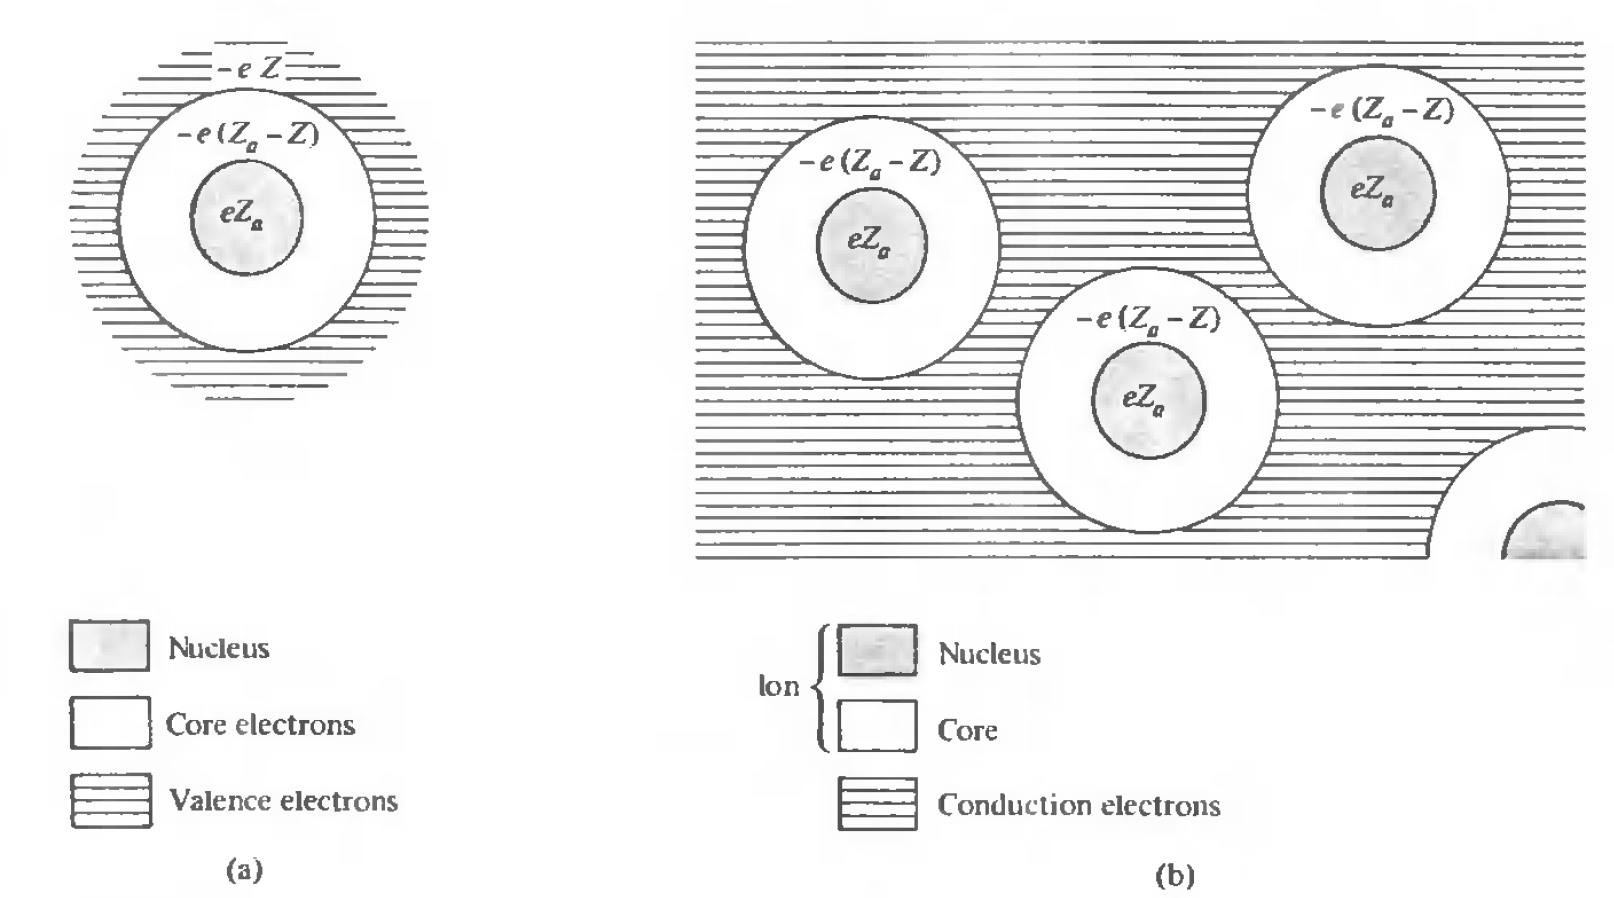
\includegraphics[width=0.9\textwidth]{figure/Drude_Model.png}
                \caption{(a)图表示单个原子的物理图像;(b)图表示金属的物理图像,可以看到价电子(valence electrons)离开原子形成电子气}
                \label{fig:DrudeModel}
            \end{figure}
                
                 Drude模型的核心是将金属中的价电子类比于理想气体的分子,运用分子动理论(kinetic theory)处理问题。根据这个指导思想,他提出了三点假设:
            \begin{enumerate}
                \item 独立电子近似(又称单电子近似):忽略了电子-电子间的相互作用;
                \item 自由电子近似:忽略了电子与离子实的相互作用;
                \item 碰撞与弛豫时间近似:电子只通过与周围电子的碰撞达到热平衡,同时碰撞的瞬间电子的速度就被迅速的改变。在单位时间内以$\frac{1}{\tau}$的概率碰撞\footnote{从电子的分布上来考虑,碰撞促使对平衡的偏离指数型的消失,即对于分布函数$f$,满足:
                \begin{equation*}
                    f=f_0e^{-\frac{t}{\tau}}
                \end{equation*}}
                
                其中$\tau$表示弛豫时间,指电子与离子实两次碰撞的平均时间间隔。这个近似表明碰撞后的速度与碰撞前的位移与速度无关,只与温度有关。同时这个近似还隐藏了一个假设:电子是经典粒子,其速度分布服从Maxwell-Bolzmann分布。
            \end{enumerate}
            
            这三个假设中,前两个假设表示金属中的价电子可以被视为理想气体分子,这种类比也被称为金属自由电子气;第三个假设说明了电子是如何达到热平衡的,同时也阐述了电子的输运性质。
            
           因为我们将电子与经典理想气体做了类比,于是我们就可以得到电子的经典运动方程了。假设t时刻电子的动量为$p(t)$,经过无穷小的时间间隔$dt$后电子的动量为$p(t+dt)$。电子在dt时间间隔内的碰撞概率为$\frac{dt}{\tau}$,不被碰撞的概率为$1-\frac{dt}{\tau}$。假设电子受到外力$f(t)$的作用(我们讨论的外力作用主要均匀外磁场和均匀外加电场产生的洛伦兹力的作用),对应的冲量为$f(t)dt$。那么经过碰撞后的体系的动量可以表示碰撞的贡献+未被碰撞的贡献,由于我们不知道碰撞的具体机制,所以我们在此忽略碰撞的贡献\footnote{或者说由于有系数$\frac{dt}{\tau}$的存在,我们可以认为碰撞的贡献都是$o(dt)^2$,因此忽略碰撞的贡献是合理的。}:
            \begin{align}\label{electron_motion_equation}
                \begin{split}
                     p(t+dt)=&\Big(1-\frac{dt}{\tau}\Big)[p(t)+f(t)dt+o(dt)^2]\\
                     \frac{p(t+dt)-p(t)}{dt}=&-\frac{p(t)}{\tau}-f(t)\\
                     \frac{dp}{dt}=&-\frac{p(t)}{\tau}+f(t)
                \end{split}
            \end{align}
            
            上述方程说明了一个简单的现象:单个电子碰撞的影响是在运动方程中为每个电子的动量引入一个摩擦阻尼项$f(t)$。根据电子的经典运动方程,结合Drude模型的假设,我们能够非常好的解释金属的直流电导率(DC conductivity)、Hall效应和热导率。
            
            \subsubsection{直流电导率与Ohm定律}
            
            首先我们讨论的金属的直流电导率\footnote{也就是说,我们考虑的电场不随时间而改变},我们从耳熟能详的欧姆定律(Ohm's Law)讲起,它说明了导线(wire)两端的电势与导线内的电流呈正比,系数$R$被称为导线的电阻(the resistance of the wire):
            \begin{equation}
                V=IR
            \end{equation}
            
            随着科学家们对电微观性质的继续探索,欧姆定律的公式也随之改变:
            \begin{equation}\label{equ:Ohm'sLaw}
                \vec{E}=\rho \vec{j}
            \end{equation}
            
            其中$\vec{E}$是单位长度的电场强度,$\vec{j}$是电流密度,它的定义是单位时间,单位有效面积(即垂直于电流方向的面积)通过的电流;比例系数$\rho$被称作电阻率(resistivity)。下面我们将利用Drude模型来得到欧姆定律(即证明电场强度$\vec{E}$和电流密度$\vec{j}$的正比关系)。
            
            我们假设金属电子的数密度为n,并且它们的速度都为v,那么在无穷小时间$dt$内通过有效面积A的电流为$-nevdt$(带负号的原因是电子带负电荷),则根据电流密度的定义,我们可以得到:
            \begin{equation}\label{currentdensity}
                \vec{j}=-ne\vec{v}
            \end{equation}
            
            对于金属中的任意一点,电子运动的方向应该是任意的。因此在没有外加电场的情况下,电子的平均速度$v_{avg}=0$\footnote{根据电子的经典运动方程\eqref{electron_motion_equation}式,我们也可以得出类似的结果,因为$\vec{j}=0$};如果施加了外加均匀电场(电场强度为E),则由于受到了洛伦兹力的作用,电子会有一个与电场方向相反的平均速度(我们称之为漂移速度(draft velocity))。根据电子的经典运动方程\eqref{electron_motion_equation}式,同时我们考虑在稳态下的情况(即$\frac{dp}{dt}=0$),我们可以得到此时电子的平均速度:
            \footnote{我们也可以根据牛顿第二定律求解:\begin{align*}
                    F=&-eE=ma=m\frac{v_{avg}}{\tau}\\
                    v_{avg}=&-\frac{eE\tau}{m}
            \end{align*}}
            
            \begin{align}
                \begin{split}
                    p(t)=&f(t)\tau\\
                    \Rightarrow mv_{avg}=&-eE\tau\\
                     \Rightarrow v_{avg}=&-\frac{eE\tau}{m}
                \end{split}
            \end{align}
               

            代入\eqref{currentdensity}式中,可以得到:
            \begin{equation}
                \vec{j}=\frac{ne^2\tau}{m}\vec{E}=\sigma\vec{E}
            \end{equation}
            
             可以看到$\sigma=\frac{ne^2\tau}{m}$是一个只与电子特性有关的常数,我们称其为电导率(conductivity)。很自然的,电导率$\sigma$和电阻率$\rho$的关系为倒数:
             \begin{equation}
                 \sigma = \frac{1}{\rho}
             \end{equation}
             
             \subsubsection{Hall效应}
                下面我们在Ohm's Law 的基础上考虑磁效应的影响。Hall效应是1879年由Hall发现的电磁学现象:他将均匀磁场作用于通电的导体中(如图\ref{fig:Halleffect}),电流中的电子受到Lorenz力的作用发生偏转,逐渐堆积在导体的一侧,直到产生稳定的电势。此时积累电子生成的电场力等于Lorenz力,受力平衡。
                \begin{figure}[H]
                    \centering
                    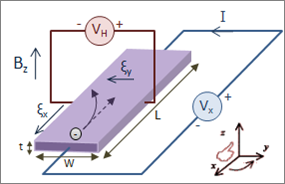
\includegraphics[width=0.7\textwidth]{figure/Hall_Effect.png}
                    \caption{Hall效应示意图}
                    \label{fig:Halleffect}
                \end{figure}
                
                根据图\ref{fig:Halleffect},我们可以知道在x,y方向上都存在电场。对于x方向上的电场,根据\eqref{equ:Ohm'sLaw}式可以得到磁阻(magnetoresistance)的定义:
                \begin{equation}
                    \rho(\vec{B})=\frac{E_x}{j_x}
                \end{equation}
                
                另一个比例常数自然与y方向上的电场有关。由于电场同时平衡了Lorenz力,因此我们猜想,除了与x方向上的电流密度$j_x$成正比,还应该和磁通量强度B成正比,于是我们可以得到Hall系数的定义:
                \begin{equation}
                    R_H=\frac{E_y}{j_xB_z}
                \end{equation}
                
                这个系数对于表征Hall效应有重要意义。下面我们根据经典力学的方法推导Hall系数,出发点仍然是电场力与磁场产生的Lorenz的平衡关系:
                \begin{equation}
                    -eE_y=-e(-v_x)B_z
                \end{equation}
                
                由此我们可以得到y方向上的电场强度$E_y$:
                \begin{equation}
                    E_y=-v_xB_z
                \end{equation}
                
                结合\eqref{currentdensity}式,我们就可以得到Hall系数的表达:
                \begin{equation}
                    R_H=\frac{E_y}{j_xB_z}=R_H=\frac{-v_xB_z}{j_xB_z}=\frac{-v_xB_z}{n(-e)(-v_x)B_z}=-\frac{1}{ne}
                \end{equation}
                
                由此我们可以知道Hall系数与金属的种类无关,只与载流子种类和密度有关。接下来我们利用Drude模型的假设得到相同的结论。
                
                我们的出发点是自由电子的经典运动方程(\eqref{electron_motion_equation}式),此时外力$f(t)$就是Lorenz力,于是运动方程可以改写为:
                \begin{equation}
                    \frac{d\vec{p}}{dt}=-\frac{\vec{p}}{\tau}-e(\vec{E}+\vec{v}\times \vec{B})=-\frac{\vec{p}}{\tau}-e(\vec{E}+\frac{\vec{p}}{m}\times \vec{B})
                \end{equation}
                
                当洛伦兹力与电场力达到平衡时,系统处于稳态,即$\frac{dp}{dt}=0$,并且将上式写成分量形式:
                \begin{align}
                    \begin{split}
                        -eE_x-\omega_cp_y-\frac{p_x}{\tau}=&0\\
                        -eE_y+\omega_cp_x-\frac{p_y}{\tau}=&0
                    \end{split}
                \end{align}
                
                其中:
                \begin{equation}
                    \omega_c=\frac{eB_z}{m}
                \end{equation}
                
                考虑到电流密度$\vec{j}=-ne\vec{v},\sigma_0=\frac{ne^2\tau}{m}$\footnote{直流电导率用$\sigma_0$表示其不随时间变化},因此在分量方程等号两端同时乘以$\frac{ne\tau}{m}$,得到:
                \begin{align}\label{equ:5A}
                    \begin{split}
                        \sigma_0E_x=&\omega_c\tau j_y+j_x\\
                        \sigma_0E_y=&-\omega_c\tau j_x +j_y
                    \end{split}
                \end{align}
                
                由于横向电流$j_y=0$,于是:
                \begin{equation}
                    E_y=-\Big(\frac{\omega_c\tau}{\sigma_0}\Big)j_x=-\Big(\frac{B_z}{ne}\Big)j_x
                \end{equation}
                
                根据Hall系数的定义就可以得到相同的结果。此外,根据\eqref{equ:5A}式,我们可以简单讨论$\omega_c\tau$的物理含义,因为这个量在后面章节的讨论中会有应用。可以看到,当$\omega_c\tau$是一个小量时,电场强度$\vec{E}$与$\vec{j}$几乎成正比,即回归到Ohm's Law,此时的情况回归到了无磁场;而在一般情况下,由于磁场的作用,$\vec{E}$和$\vec{j}$并不平行,它们之间存在一个角度$\phi$(被称作Hall angle),其中角度满足公式:$\tan{\phi}=\omega_c\tau$。$\omega_c$的大小被称作回旋频率(cyclotron frequency),我们可以将其理解为载流子在磁场B中发生旋转的角频率。因此$\omega_c\tau$可以表现为两次碰撞间发生旋转的情况,同时它的大小也直接决定磁场作用的大小。
             \subsubsection{金属的热导率,Wiedmann-Franz定律}
                本节我们讨论的金属的热导$\kappa$。1853年,Wiedmann和Franz根据实验,提出了一个经验定律:热导和直流电导的比值$\frac{\kappa}{\sigma}$与温度$T$成正比。本节我们通过Drude模型的假设对金属的热导进行分析,并证明Wiedmann-Franz定律。
                
                那么什么是热导率呢?我们可以将其与电现象相类比:所谓电导/电阻,就是衡量电流通过的容易程度;那么热导率的引入,自然就是衡量热流通过物理容易的程度。这个概念的引入是基于当时科学家观察到金属的导热性要好于绝缘体(insulator)的实验现象。根据实验现象,科学家总结出了所谓Fourier定律的经验公式:
                \begin{equation}
                    \vec{j^q}=-\kappa\nabla T
                \end{equation}
                
                上式中$\nabla T$代表温度的梯度,而负号则说明热流是从物体温度高处流向温度低处。该式是我们讨论的基础,下面我们就从微观角度重新认识一下热流:根据碰撞理论,如果某个区域温度越高,那么这个区域碰撞的次数越多,电子的能量越大。因此即使电子的方均根速度为零,但是整体上电子还是从温度高的地方流向温度低的地方。
                
                下一步我们进行定量的分析\footnote{这里为了讨论的方便,定量的讨论限制在一维的情况}。在定量分析中,我们同样将热流与电流做类比。根据\eqref{currentdensity}式,我们可以知道,对于热流,同样有类似的结论:
                \begin{equation}
                    \text{热流}\vec{j^q}=\text{数密度}n\cdot \text{电子速度}v \cdot \text{每个电子携带的能量}
                \end{equation}
                
                那么问题就转化为了如何计算每个电子携带的能量。我们研究数密度为n,在$x$处的净热流。假设当温度为$T$时,在$x$平均每个电子在经过最后一次碰撞后,达到平衡时的内能为$\varepsilon(T[x])$;该处内能等于流入的电子携带的内能减去流出的电子携带的内能。虽然电子存在速度分布,但是在弛豫时间$\tau$内,我们往往使用一种“平均”速度$v$来代表所有符合要求电子的速度。于是流入的电子在经过最后一次碰撞后达到平衡时的内能为$\varepsilon(T[x-v\tau])$;同理,流出电子在经过最后一次碰撞后达到平衡时的内能为$\varepsilon(T[x+v\tau])$。因此在$x$处的净热流可以表示为:
                \begin{equation}
                    j^q=\frac{1}{2}nv[\varepsilon(T[x-v\tau])-\varepsilon(T[x+v\tau])]
                \end{equation}
                
                该式中$\frac{1}{2}$是因为流入与流出电子的数密度贡献各占一半。由于体系的平均自由程$l=v\tau$是一个小量,因此我们可以对上式进行泰勒展开,可得:
                \begin{align}
                    \begin{split}
                        j^q=&\frac{1}{2}nv[\varepsilon(T[x])-v\tau \frac{d\varepsilon}{dx}-\varepsilon(T[x])-v\tau\frac{d\varepsilon}{dx}]\\
                        =&nv^2\tau\Big(-\frac{d\varepsilon}{dx}\Big)\\
                        =&nv^2\tau\frac{d\varepsilon}{dT}\Big(-\frac{dT}{dx}\Big)\\
                        =&C_{v,N}v^2\tau\Big(-\frac{dT}{dx}\Big)
                    \end{split}
                \end{align}
                    
                其中:
                \begin{equation}
                    n\frac{d\varepsilon}{dT}=\frac{N}{V}\frac{d\varepsilon}{dT}=\frac{1}{V}\frac{dE}{dT}=C_{v,N}
                \end{equation}
                
                对于三维情况,由于各个方向上的方均根速度都是相等的($\langle v_x^2\rangle=\langle v_y^2\rangle=\langle v_z^2\rangle=\frac{1}{3}\vec{v}^2$),所以我们可以很容易地将上式推广到三维情况:
                \begin{equation}
                    \vec{j^q}=\frac{1}{3}v^2\tau C_{v,N}(-\nabla T)
                \end{equation}
                
                对比Fourier's Law($\vec{j^q}=-\kappa\nabla T$),我们可以得到热导率$\kappa$的表达式:
                \begin{equation}
                    \kappa=\frac{1}{3}v^2\tau C_{v,N}
                \end{equation}
                
                结合经典统计力学中热容的表达($C_{v,N}=\frac{3}{2}nk_B$),内能的恒等式($\frac{1}{2}mv^2=\frac{3}{2}k_BT$)和直流电导率的表达式($\sigma=\frac{ne^2\tau}{m}$),我们可以验证Wiedmann-Franz定律:
                \begin{equation}
                    \frac{\kappa}{\sigma}=\frac{\frac{1}{3}C_{v,N}mv^2}{ne^2}=\frac{3}{2}\Big(\frac{k_B}{e}\Big)^2T
                \end{equation}
                
                其中,上式中$k_B$和$e$都是普遍的常数,于是热导率和电导率的比值就和温度成正比。
             \subsubsection{Drude模型的不足}
                虽然Drude模型已经能够解释很多现象,但是随着实验手段的发展,越来越多的现象无法用Drude模型解释:
                \begin{enumerate}
                    \item 根据Drude模型,电子的摩尔热容应该恒等于$\frac{3}{2}R$,与晶格振动热容一样,但是实验测得,在300K时,电子的摩尔热容为0.03R,远小于理论值;
                    \item 根据Drude模型,我们得到了电导率的公式$\sigma=\frac{ne^2}{m}\tau$,其中$n,e,m$都是普遍常量,但是由于弛豫时间$\tau$与电子的速度成反比,于是结合M-B分布平均速率的结论$v\propto T^{\frac{1}{2}}$,我们可以得到电导率与温度的满足:
                    \begin{equation}
                        \sigma\propto \tau \propto \frac{1}{v}\propto T^{-\frac{1}{2}}
                    \end{equation}
                    
                    这与实验结论电导率与温度成反比($\sigma\propto T^{-1}$)不符合。
                    \item 在前面我们已经知道Drude模型能很好的解释Wiedmann-Franz定律,即$\frac{\kappa}{\sigma}$与温度$T$成正比。但是问题在于,当我们考虑与定律密切相关的洛伦兹数$L$时,我们发现其数值与实验存在误差:
                    \begin{equation}
                        L=\frac{\kappa}{\sigma T}=\frac{3}{2}\Big(\frac{k_B}{e}\Big)^2=1.11\times 10^{-8}J^2\cdot C^{-2}\cdot K^{-2}
                    \end{equation}
                    
                    但是根据实验结果,洛伦兹数L的大小为$2.22\times 10^{-8}$,应该正好是Drude模型推导结果的一倍,这个系统性误差难以解释。
                \end{enumerate}
                
                究其原因,一方面是由于Drude模型研究的对象电子是满足量子力学规律的粒子,使用经典粒子去描述必然产生误差;另一方面则是由于Drude模型的假设过于粗糙,忽略了太多的内容。下一节的Sommerfeld模型就是解决了前者;而下一章——能带论则是在Sommerfeld模型的基础上逐步处理近似条件。
             \subsection{Sommerfeld模型}
    \end{document}
